\documentclass[a4paper,10pt]{book}
\usepackage[utf8]{inputenc}
\usepackage{physics}
\newcommand*\diff{\mathop{}\!\mathrm{d}}
\usepackage{fullpage}
\usepackage{cite}
\usepackage[utf8]{inputenc}
\usepackage{a4wide}
\usepackage{url}
\usepackage{graphicx}
\usepackage{caption}
\usepackage{float} % para que los gr\'aficos se queden en su lugar con [H]
\usepackage{subcaption}
\usepackage{wrapfig}
\usepackage{color}
\usepackage{amsmath} %para escribir funci\'on partida , matrices
\usepackage{amsthm} %para numerar definciones y teoremas
\usepackage[hidelinks]{hyperref} % para inlcuir links dentro del texto
\usepackage{tabu} 
\usepackage{comment}
\usepackage{amsfonts} % \mathbb{N} -> conjunto de los n\'umeros naturales  
\usepackage{enumerate}
\usepackage{listings}
\usepackage[colorinlistoftodos, textsize=small]{todonotes} % Para poner notas en el medio del texto!! No olvidar hacer. 
\usepackage{framed} % Para encuadrar texto. \begin{framed}
\usepackage{csquotes} % Para citar texto \begin{displayquote}
\usepackage{epigraph} % Epigrafe  \epigraph{texto}{\textit{autor}}
\usepackage{authblk}
\usepackage{titlesec}
\usepackage{varioref}
\usepackage{bm} % \bm{\alpha} bold greek symbol
\usepackage{pdfpages} % \includepdf
\usepackage[makeroom]{cancel} % \cancel{} \bcancel{} etc
\usepackage{wrapfig} % \begin{wrapfigure} Pone figura al lado del texto
\usepackage{mdframed}
\usepackage{algorithm}
%\usepackage{quoting}
\usepackage{mathtools}	
\usepackage{tikz}
\usepackage{paracol}
\usepackage[binary-units]{siunitx} % \num{} \SI{}
% tikzlibrary.code.tex
%
% Copyright 2010-2011 by Laura Dietz
% Copyright 2012 by Jaakko Luttinen
%
% This file may be distributed and/or modified
%
% 1. under the LaTeX Project Public License and/or
% 2. under the GNU General Public License.
%
% See the files LICENSE_LPPL and LICENSE_GPL for more details.

% Load other libraries

%\newcommand{\vast}{\bBigg@{2.5}}
% newcommand{\Vast}{\bBigg@{14.5}}
% \usepackage{helvet}
% \renewcommand{\familydefault}{\sfdefault}

\usetikzlibrary{shapes}
\usetikzlibrary{fit}
\usetikzlibrary{chains}
\usetikzlibrary{arrows}

% Latent node
\tikzstyle{latent} = [circle,fill=white,draw=black,inner sep=1pt,
minimum size=20pt, font=\fontsize{10}{10}\selectfont, node distance=1]
% Observed node
\tikzstyle{obs} = [latent,fill=gray!25]
% Invisible node
\tikzstyle{invisible} = [latent,minimum size=0pt,color=white, opacity=0, node distance=0]
% Constant node
\tikzstyle{const} = [rectangle, inner sep=0pt, node distance=0.1]
%state
\tikzstyle{estado} = [latent,minimum size=8pt,node distance=0.4]
%action
\tikzstyle{accion} =[latent,circle,minimum size=5pt,fill=black,node distance=0.4]
\tikzstyle{fijo} =[latent,circle,minimum size=5pt,fill=black]


% Factor node
\tikzstyle{factor} = [rectangle, fill=black,minimum size=10pt, draw=black, inner
sep=0pt, node distance=1]
% Deterministic node
\tikzstyle{det} = [latent, rectangle]

% Plate node
\tikzstyle{plate} = [draw, rectangle, rounded corners, fit=#1]
% Invisible wrapper node
\tikzstyle{wrap} = [inner sep=0pt, fit=#1]
% Gate
\tikzstyle{gate} = [draw, rectangle, dashed, fit=#1]

% Caption node
\tikzstyle{caption} = [font=\footnotesize, node distance=0] %
\tikzstyle{plate caption} = [caption, node distance=0, inner sep=0pt,
below left=5pt and 0pt of #1.south east] %
\tikzstyle{factor caption} = [caption] %
\tikzstyle{every label} += [caption] %

\tikzset{>={triangle 45}}

%\pgfdeclarelayer{b}
%\pgfdeclarelayer{f}
%\pgfsetlayers{b,main,f}

% \factoredge [options] {inputs} {factors} {outputs}
\newcommand{\factoredge}[4][]{ %
  % Connect all nodes #2 to all nodes #4 via all factors #3.
  \foreach \f in {#3} { %
    \foreach \x in {#2} { %
      \path (\x) edge[-,#1] (\f) ; %
      %\draw[-,#1] (\x) edge[-] (\f) ; %
    } ;
    \foreach \y in {#4} { %
      \path (\f) edge[->,#1] (\y) ; %
      %\draw[->,#1] (\f) -- (\y) ; %
    } ;
  } ;
}

% \edge [options] {inputs} {outputs}
\newcommand{\edge}[3][]{ %
  % Connect all nodes #2 to all nodes #3.
  \foreach \x in {#2} { %
    \foreach \y in {#3} { %
      \path (\x) edge [->,#1] (\y) ;%
      %\draw[->,#1] (\x) -- (\y) ;%
    } ;
  } ;
}

% \factor [options] {name} {caption} {inputs} {outputs}
\newcommand{\factor}[5][]{ %
  % Draw the factor node. Use alias to allow empty names.
  \node[factor, label={[name=#2-caption]#3}, name=#2, #1,
  alias=#2-alias] {} ; %
  % Connect all inputs to outputs via this factor
  \factoredge {#4} {#2-alias} {#5} ; %
}

% \plate [options] {name} {fitlist} {caption}
\newcommand{\plate}[4][]{ %
  \node[wrap=#3] (#2-wrap) {}; %
  \node[plate caption=#2-wrap] (#2-caption) {#4}; %
  \node[plate=(#2-wrap)(#2-caption), #1] (#2) {}; %
}

% \gate [options] {name} {fitlist} {inputs}
\newcommand{\gate}[4][]{ %
  \node[gate=#3, name=#2, #1, alias=#2-alias] {}; %
  \foreach \x in {#4} { %
    \draw [-*,thick] (\x) -- (#2-alias); %
  } ;%
}

% \vgate {name} {fitlist-left} {caption-left} {fitlist-right}
% {caption-right} {inputs}
\newcommand{\vgate}[6]{ %
  % Wrap the left and right parts
  \node[wrap=#2] (#1-left) {}; %
  \node[wrap=#4] (#1-right) {}; %
  % Draw the gate
  \node[gate=(#1-left)(#1-right)] (#1) {}; %
  % Add captions
  \node[caption, below left=of #1.north ] (#1-left-caption)
  {#3}; %
  \node[caption, below right=of #1.north ] (#1-right-caption)
  {#5}; %
  % Draw middle separation
  \draw [-, dashed] (#1.north) -- (#1.south); %
  % Draw inputs
  \foreach \x in {#6} { %
    \draw [-*,thick] (\x) -- (#1); %
  } ;%
}

% \hgate {name} {fitlist-top} {caption-top} {fitlist-bottom}
% {caption-bottom} {inputs}
\newcommand{\hgate}[6]{ %
  % Wrap the left and right parts
  \node[wrap=#2] (#1-top) {}; %
  \node[wrap=#4] (#1-bottom) {}; %
  % Draw the gate
  \node[gate=(#1-top)(#1-bottom)] (#1) {}; %
  % Add captions
  \node[caption, above right=of #1.west ] (#1-top-caption)
  {#3}; %
  \node[caption, below right=of #1.west ] (#1-bottom-caption)
  {#5}; %
  % Draw middle separation
  \draw [-, dashed] (#1.west) -- (#1.east); %
  % Draw inputs
  \foreach \x in {#6} { %
    \draw [-*,thick] (\x) -- (#1); %
  } ;%
}




\definecolor{julia}{rgb}{1, 0.5, 1}
\definecolor{python}{rgb}{1, 1, 0.5}
\definecolor{r}{rgb}{0.70, 0.80, 1}
\definecolor{all}{rgb}{0.85, 0.85, 0.85}


\usepackage{listings}
\lstset{
  aboveskip=3mm,
  belowskip=3mm,
  showstringspaces=true,
  columns=flexible,
  basicstyle={\footnotesize\ttfamily},
  breaklines=true,
  breakatwhitespace=true,
  tabsize=4,
  showlines=true
}

\hypersetup{
    colorlinks,
    linkcolor={black!50!black},
    citecolor={black!50!black},
    urlcolor={black!80!black}
}


\newcommand{\vm}[1]{\mathbf{#1}}
\newcommand{\N}{\mathcal{N}}
\newcommand{\citel}[1]{\cite{#1}\label{#1}}
\newcommand\hfrac[2]{\genfrac{}{}{0pt}{}{#1}{#2}} %\frac{}{} sin la linea del medio

\newtheorem{midef}{Definition}
\newtheorem{miteo}{Theorem}
\newtheorem{mipropo}{Proposition}

\theoremstyle{definition}
\newtheorem{definition}{Definition}[section]
\newtheorem{theorem}{Theorem}[section]
\newtheorem{proposition}{Proposition}[section]

%http://latexcolor.com/
\definecolor{azul}{rgb}{0.36, 0.54, 0.66}
\definecolor{rojo}{rgb}{0.7, 0.2, 0.116}
\definecolor{rojopiso}{rgb}{0.8, 0.25, 0.17}
\definecolor{verdeingles}{rgb}{0.12, 0.5, 0.17}
\definecolor{ubuntu}{rgb}{0.44, 0.16, 0.39}
\definecolor{debian}{rgb}{0.84, 0.04, 0.33}
\definecolor{dkgreen}{rgb}{0,0.6,0}
\definecolor{gray}{rgb}{0.5,0.5,0.5}
\definecolor{mauve}{rgb}{0.58,0,0.82}

\newif\ifen
\newif\ifes
\newcommand{\en}[1]{\ifen#1\fi}
\newcommand{\es}[1]{\ifes#1\fi}
\estrue


%opening
\title{\huge Algoritmos para la inferencia de habilidad y el aprendizaje social}
\author{Gustavo Landfried}


\begin{document}

\maketitle

\tableofcontents


\chapter{Conocimiento empírico}

\epigraph{El conocimiento empírico no es más que principio de indiferencia compatible con la evidencia formal y empírica}{}

La ciencia es una institución humana que tiene pretención de verdad.
Las ciencias formales validan sus proposiciones mediante teoremas, resultados derivados de aplicar las reglas internas a un sistema axiomático cerrado.
Las ciencias empíricas, por el contrario, deben validar sus proposiciones dentro de sistemas abiertos, lo que impone siempre un grado de incertidumbre asociada.
¿Cuál es entonces la fuente de validez del conocimiento empírico?

\section{Principio de indiferencia}

Supongamos que tenemos tres cajas y sólo sabemos que detrás de una hay un regalo.
Para expresar nuestra (in)certidumbre repartiremos la creencia entre las posibles opciones.
A las diferentes formas de dividir la creencia le vamos a llamar \emph{distribución de creencias}.
Una posible distirbución de creencias es,
%
\begin{figure}[H]
\centering
\tikz{ %
        
         \node[factor, minimum size=1cm] (p1) {} ;
         \node[factor, minimum size=1cm, xshift=1.5cm] (p2) {} ;
         \node[factor, minimum size=1cm, xshift=3cm] (p3) {} ;
         \node[const, above=of p1, yshift=.15cm] (fp1) {$1/10$};
         \node[const, above=of p2, yshift=.15cm] (fp2) {$8/10$};
         \node[const, above=of p3, yshift=.15cm] (fp3) {$1/10$};
        } 
\end{figure}
%
lo que representa una preferencia parcial por la caja del medio.
Pero si de verdad no tenemos ninguna información respecto de dónde está el regalo, no hay motivos para tener preferencia por ninguna de las opciones, lo que sin lugar a dudas nos hará estar de acuerdo en la necesidad de dividir la creencia en partes iguales.
Éste es un principio de validez intercultural conocido como ``de indiferencia''.
%
\begin{figure}[H]
\centering
\tikz{ %
        
         \node[factor, minimum size=1cm] (p1) {} ;
         \node[factor, minimum size=1cm, xshift=1.5cm] (p2) {} ;
         \node[factor, minimum size=1cm, xshift=3cm] (p3) {} ;
         \node[const, above=of p1, yshift=.15cm] (fp1) {$1/3$};
         \node[const, above=of p2, yshift=.15cm] (fp2) {$1/3$};
         \node[const, above=of p3, yshift=.15cm] (fp3) {$1/3$};
        } 
\end{figure}

Este tipo de distribuciones de creencias, que permiten el acuerdo intersubjetivo, la vamos a llamar \textbf{creencia honesta}.
Elegimos el término ``intersubjetividad'', por sobre el de ``subjetividad'', debido a que el primero connota el cumplimiento de las condiciones que producen al acuerdo entre las conciencias individuales, mientras que el segundo connota una arbitrariedad que lo obstaculiza.
Elegimos el término ``intersubjetividad'', por sobre el de ``objetividad'', porque el primero connota una actividad construcitva entre los sujetos, mientras que el segundo connota la imposición directa del objeto sobre los sujetos.

% Parrafo

%Una propiedad común a todas las creencias honestas es la maximización de la incertidumbre (manteniendo la coherencia con la información disponible).
%La distribución con menor incertidumbre es la que asigna toda la creencia a una de las opciones.
%La distirbución más lejana a esta, 
%En este caso, en el que no tenemos información previa, la obtuvimos dividiendo la creencia en partes iguales.
Tenemos entonces un principio para alcanzar acuerdos en los casos en los que no tenemos información previa.
¿Pero cómo hacemos para alcanzar acuerdos cuando recibimos nueva información?

\section{Evidencia formal y empirica}

Supongamos que recibimos el dato (i.e. tenemos la certeza) de que el regalo no está en la caja del medio.
En este caso es fácil llegar a un acuerdo que nos permita asignar creencia 0 a la caja del medio.
%
\begin{figure}[H]
\centering
\tikz{ %
         \node[factor, minimum size=1cm] (p1) {} ;
         \node[det, minimum size=1cm, xshift=1.5cm] (p2) {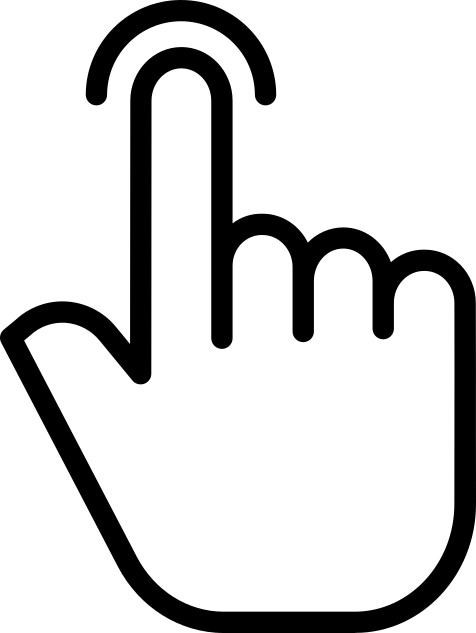
\includegraphics[width=0.03\textwidth]{static/dedo.png}} ;
         \node[factor, minimum size=1cm, xshift=3cm] (p3) {} ;

         \node[const, above=of p1, yshift=.15cm] (fp1) {$?$};
         \node[const, above=of p2, yshift=.15cm] (fp2) {$0$};
         \node[const, above=of p3, yshift=.15cm] (fp3) {$?$};
         \node[const, below=of p2, yshift=-.10cm, xshift=0.3cm] (dedo) {};
        } 
\end{figure}
%
Para actualizar el resto de las cajas necesitamos interpretar qué nos está diciendo la pista.
Supongamos que la pista depende de dónde está el regalo, sólo nos puede indicar dónde no está el regalo.
Esto lo podemos representar con el siguiente modelo causal.
%
\begin{figure}[H]
\centering
\tikz{            
    \node[latent,] (r) {
\includegraphics[width=0.06\textwidth]{static/regalo.png}} ;
    \node[const,left=of r] (nr) {\Large $r$} ;    
    
    
    \node[latent, below=of r] (d) {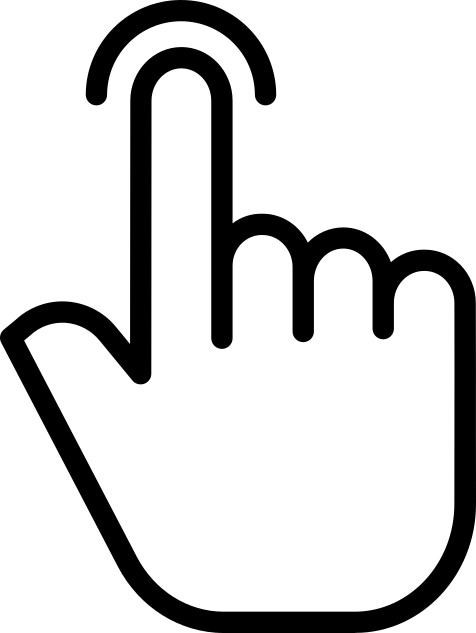
\includegraphics[width=0.05\textwidth]{static/dedo.png}} ;
    \node[const, left=of d] (nd) {\Large $s$} ;

    \edge {r} {d};
            
}
\end{figure}
%
Lo que está diciendo este modelo gráfico es: ``la pista $s$ depende del regalo $r$''.
Si tenemos la certeza de que el regalo $r$ está en la caja $i$ y que la pista $s$ nunca señalará la misma caja donde se ubica el regalo, será fácil llegar a un acuerdo que nos permita asignar creencia 0 a ese evento.
%
\begin{equation}
\text{Creencia}(s=i|r=i) = 0
\end{equation}
%

%
Siguiendo con el principio de indiferencia que usamos para definir una creencia honesta, dividimos la creencia en partes iguales por los caminos del modelo causal para definir la creencia honesta de ellos.

\begin{figure}[H]
\centering
\tikz{
\node[latent, draw=white, yshift=0.6cm] (b0) {$1$};

\node[latent,below=of b0,yshift=0.6cm, xshift=-3cm] (r1) {$r_1$};
\node[latent,below=of b0,yshift=0.6cm] (r2) {$r_2$};
\node[latent,below=of b0,yshift=0.6cm, xshift=3cm] (r3) {$r_3$};

\node[latent, below=of r1, draw=white, yshift=0.6cm] (br1) {$\frac{1}{3}$};
\node[latent, below=of r2, draw=white, yshift=0.6cm] (br2) {$\frac{1}{3}$};
\node[latent, below=of r3, draw=white, yshift=0.6cm] (br3) {$\frac{1}{3}$};
\node[latent,below=of br1,yshift=0.6cm, xshift=-0.7cm] (r1d2) {$s_2$};
\node[latent,below=of br1,yshift=0.6cm, xshift=0.7cm] (r1d3) {$s_3$};

\node[latent,below=of r1d2,yshift=0.6cm,draw=white] (br1d2) {$\frac{1}{3}\frac{1}{2}$};
\node[latent,below=of r1d3,yshift=0.6cm, draw=white] (br1d3) {$\frac{1}{3}\frac{1}{2}$};
\node[latent,below=of br2,yshift=0.6cm, xshift=-0.7cm] (r2d1) {$s_1$};
\node[latent,below=of br2,yshift=0.6cm, xshift=0.7cm] (r2d3) {$s_3$};
\node[latent,below=of br3,yshift=0.6cm, xshift=-0.7cm] (r3d1) {$s_1$};
\node[latent,below=of br3,yshift=0.6cm, xshift=0.7cm] (r3d2) {$s_2$};

\node[latent,below=of r2d1,yshift=0.6cm, draw=white] (br2d1) {$\frac{1}{3}\frac{1}{2}$};
\node[latent,below=of r2d3,yshift=0.6cm,draw=white] (br2d3) {$\frac{1}{3}\frac{1}{2}$};
\node[latent,below=of r3d1,yshift=0.6cm, draw=white] (br3d1) {$\frac{1}{3}\frac{1}{2}$};
\node[latent,below=of r3d2,yshift=0.6cm,draw=white] (br3d2) {$\frac{1}{3}\frac{1}{2}$};
\edge[-] {b0} {r1,r2,r3};
\edge[-] {r1} {br1};
\edge[-] {r2} {br2};
\edge[-] {r3} {br3};
\edge[-] {br1} {r1d2,r1d3};
\edge[-] {r1d2} {br1d2};
\edge[-] {r1d3} {br1d3};
\edge[-] {br2} {r2d1, r2d3};
\edge[-] {br3} {r3d1,r3d2};
\edge[-] {r2d1} {br2d1};
\edge[-] {r2d3} {br2d3};
\edge[-] {r3d1} {br3d1};
\edge[-] {r3d2} {br3d2};
}
\end{figure}

Primero dividimos la creencia sobre el regalo en partes iguales, y luego volvemos a dividir la creencia sobre la pista en partes iguales.
\todo[inline]{Explicar, la verdad es que no decis nada en el texto, contalo para alguien que no tiene porque saber nada}
Nuestra creencia conjunta honesta a priori es,

\begin{table}[H]
\centering
 \begin{tabular}{c|c|c|c|} \setlength\tabcolsep{0.4cm} 
        & \, $r_1$ \, &  \, $r_2$ \, & \, $r_3$ \, \\ \hline 
  $s_1$ & $0$ & $1/6$ & $1/6$  \\ \hline
  $s_2$ & $1/6$ & $0$ & $1/6$  \\ \hline
  $s_3$ & $1/6$ & $1/6$ & $0$ \\ \hline 
  \end{tabular}
\end{table}
  
Es honesta porque maximiza la incertidumbre dada la información disponible hasta el momento: el modelo causal.
Y es conjunta porque es la creencia de que ocurran simultaneamente ambas variables, $\text{Creencia}(r,s)$.
\todo[inline]{el parrafo anterior y la tabla hay que explicarla, asi como esta no se entiende}

% Parrafo

Habiendo definido la creencia conjunta, las creencias sobre cada una de las variables se obtiene como el total.
La creencia sobre el regalo nuevamente es 1/3,
\begin{equation}
\text{Creencia}(r_i) = \sum_j \text{Creencia}(r_i, s_j) = 1/3
\end{equation}
y sobre la pista también
\begin{equation}
\text{Creencia}(s_j) = \sum_i \text{Creencia}(r_i, s_j) = 1/3
\end{equation}

% Parrafo

Para actualizar las creencias simplemente nos quedamos con la creencia a priori que es compatible con el dato, $\text{Creencia}(r_i, s_2)$.
%
\begin{table}[H]
\centering
 \begin{tabular}{c|c|c|c|c} \setlength\tabcolsep{0.4cm} 
        & \, $r_1$ \, &  \, $r_2$ \, & \, $r_3$ \, & \\ \hline 
  $s_1$ &  &  & & \\ \hline
  $s_2$ & $1/6$ & $0$ & $1/6$ & $1/3$ \\ \hline
  $s_3$ &  &  &  & \\ \hline 
  \end{tabular}
\end{table}
%
Lo que nos permitirá cumplir el objetivo que nos habíamos propuesto, actualizar la creencia sobre el regalo luego de haber visto la pista.
Como \textbf{la creencia que sobrevive} es ahora nuestra nueva creencia total, la normalizamos (en partes iguales) para que vuelva a sumar 1
%
\begin{equation}
\text{Creencia}(r_i| s_2) = \frac{\text{Creencia}(r_i, s_2)}{\text{Creencia}(s_2)} = 1/2
\end{equation}
%
La concusión a la que llegamos coincide con la intuición de la mayoría.
\begin{figure}[H]
\centering
\tikz{ %
        
         \node[factor, minimum size=1cm] (p1) {} ;
         \node[det, minimum size=1cm, xshift=1.5cm] (p2) {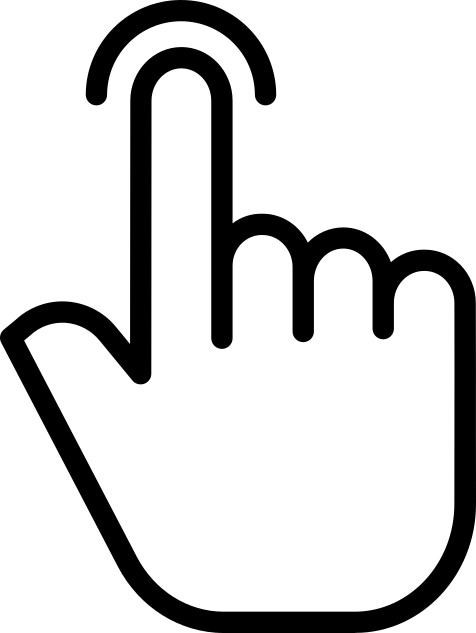
\includegraphics[width=0.03\textwidth]{static/dedo.png}} ;
         \node[factor, minimum size=1cm, xshift=3cm] (p3) {} ;

         \node[const, above=of p1, yshift=.15cm] (fp1) {$1/2$};
         \node[const, above=of p2, yshift=.15cm] (fp2) {$0$};
         \node[const, above=of p3, yshift=.15cm] (fp3) {$1/2$};
         \node[const, below=of p2, yshift=-.10cm, xshift=0.3cm] (dedo) {};
}
\end{figure}
%
Pero este resultado depende del modelo causal elegido.

\subsection{Modelos causales alternativos}

Supongamos que la pista, además de no poder coincidir con la posición del regalo, tiene prohibida una de las puertas.
Esto lo podemos representar con el siguiente modelo causal.

\begin{figure}[H]
\centering
\tikz{        
    
    \node[latent] (d) {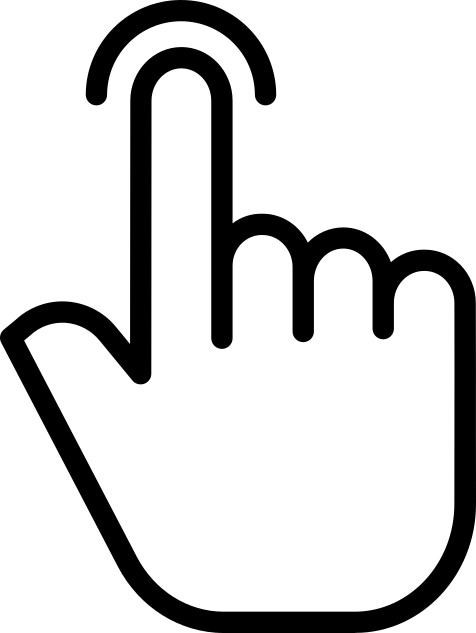
\includegraphics[width=0.05\textwidth]{static/dedo.png}} ;
    \node[const,above=of d] (nd) {\Large $s$} ;
    
    \node[latent, above=of d, xshift=-1.5cm] (r) {
\includegraphics[width=0.06\textwidth]{static/regalo.png}} ;
    \node[const,above=of r] (nr) {\Large $r$} ;
    
    \node[latent, fill=black!30, above=of d, xshift=1.5cm] (c) {
\includegraphics[width=0.06\textwidth]{static/cerradura.png}} ;
    \node[const,above=of c] (nc) {\Large $c=1$} ;
    
    \edge {r,c} {d};
}
\end{figure}

Este modelo es más conocido como el Monty Hall.
Para simplificar el problema, suponemos que la puerta 1 es la que queda cerrada, $c=1$.
Supongamos que en este contexto recibimos una pista.
%
\begin{figure}[H]
\centering
\tikz{ %
        
         \node[factor, minimum size=1cm] (p1) {
\includegraphics[width=0.025\textwidth]{static/cerradura.png}} ;
         \node[det, minimum size=1cm, xshift=1.5cm] (p2) {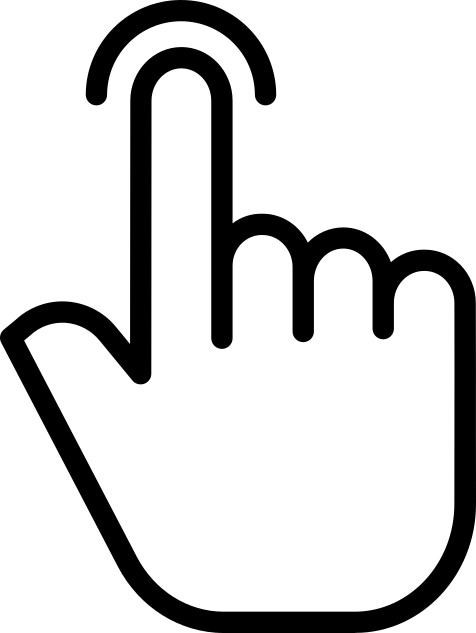
\includegraphics[width=0.03\textwidth]{static/dedo.png}} ;
         \node[factor, minimum size=1cm, xshift=3cm] (p3) {} ;
         \node[const, above=of p1, yshift=.15cm] (fp1) {$?$};
         \node[const, above=of p2, yshift=.15cm] (fp2) {$0$};
         \node[const, above=of p3, yshift=.15cm] (fp3) {$?$};
         \node[const, below=of p2, yshift=-.10cm, xshift=0.3cm] (dedo) {};
        
        } 
\end{figure}

¿Cómo hacemos para actualizar las creencias de forma honesta?
Como hicimos antes, maximizamos la incertidumbre dividiendo las creencias por los caminos del modelo causal de modo de definir la creencia conjunta honesta.

\begin{figure}[H]
\centering
\tikz{
\node[latent, draw=white, yshift=0.8cm] (b0) {$1$};
\node[latent,below=of b0,yshift=0.8cm, xshift=-2cm] (r1) {$r_1$};
\node[latent,below=of b0,yshift=0.8cm] (r2) {$r_2$};
\node[latent,below=of b0,yshift=0.8cm, xshift=2cm] (r3) {$r_3$};

\node[latent, below=of r1, draw=white, yshift=0.8cm] (br1) {$\frac{1}{3}$};
\node[latent, below=of r2, draw=white, yshift=0.8cm] (br2) {$\frac{1}{3}$};
\node[latent, below=of r3, draw=white, yshift=0.8cm] (br3) {$\frac{1}{3}$};
\node[latent,below=of br1,yshift=0.8cm] (c11) {$c_1$};
\node[latent,below=of br2,yshift=0.8cm] (c12) {$c_1$};
\node[latent,below=of br3,yshift=0.8cm] (c13) {$c_1$};

\node[latent, below=of c11, draw=white, yshift=0.8cm] (bc11) {$\frac{1}{3}$};
\node[latent, below=of c12, draw=white, yshift=0.8cm] (bc12) {$\frac{1}{3}$};
\node[latent, below=of c13, draw=white, yshift=0.8cm] (bc13) {$\frac{1}{3}$};
\node[latent,below=of bc11,yshift=0.8cm, xshift=-0.7cm] (r1d2) {$s_2$};
\node[latent,below=of bc11,yshift=0.8cm, xshift=0.7cm] (r1d3) {$s_3$};
\node[latent,below=of bc12,yshift=0.8cm] (r2d3) {$s_3$};
\node[latent,below=of bc13,yshift=0.8cm] (r3d2) {$s_2$};

\node[latent,below=of r1d2,yshift=0.8cm,draw=white] (br1d2) {$\frac{1}{3}\frac{1}{2}$};
\node[latent,below=of r1d3,yshift=0.8cm, draw=white] (br1d3) {$\frac{1}{3}\frac{1}{2}$};
\node[latent,below=of r2d3,yshift=0.8cm,draw=white] (br2d3) {$\frac{1}{3}$};
\node[latent,below=of r3d2,yshift=0.8cm,draw=white] (br3d2) {$\frac{1}{3}$};
\edge[-] {b0} {r1,r2,r3};
\edge[-] {r1} {br1};
\edge[-] {r2} {br2};
\edge[-] {r3} {br3};
\edge[-] {br1} {c11};
\edge[-] {br2} {c12};
\edge[-] {br3} {c13};
\edge[-] {c11} {bc11};
\edge[-] {c12} {bc12};
\edge[-] {c13} {bc13};
\edge[-] {bc11} {r1d2,r1d3};
\edge[-] {bc12} {r2d3};
\edge[-] {bc13} {r3d2};
\edge[-] {r1d2} {br1d2};
\edge[-] {r1d3} {br1d3};
\edge[-] {r2d3} {br2d3};
\edge[-] {r3d2} {br3d2};
}
\end{figure}

Cuando el regalo está detrás de la puerta 1, $r_1$, podemos recibir una pista tanto en la puerta 2, $s_2$, como en la puerta 3, $s_3$.
Si el regalo está en la puerta 2, $r_2$, la pista sólo puede señalar la puerta 3, $s_3$.
Así definimos la siguiente creencia honesta conjunta (y sus marginales).

\begin{table}[H]
\centering
 \begin{tabular}{c|c|c|c||c} \setlength\tabcolsep{0.4cm} 
        & \, $r_1$ \, &  \, $r_2$ \, & \, $r_3$ \, & \\ \hline 
  $s_2$ & $1/6$ & $0$ & $1/3$ & $1/2$ \\ \hline
  $s_3$ & $1/6$ & $1/3$ & $0$ & $1/2$ \\ \hline \hline 
  & $1/3$& $1/3$ & $1/3$ & $1$
  \end{tabular}
 \end{table}
 
Para actualizar nuestra creencia, nuevamente nos quedamos con la creencia a priori que es compatible con los datos.

\begin{table}[H]
\centering
 \begin{tabular}{c|c|c|c||c} \setlength\tabcolsep{0.4cm} 
        & \, $r_1$ \, &  \, $r_2$ \, & \, $r_3$ \, &  \\ \hline 
  $s_2$ & $1/6$ & $0$ & $1/3$ & $1/2$ \\ \hline
  \end{tabular}
\end{table}

Que normalizado en partes iguales para que sume 1 queda como

\begin{figure}[H]
\centering
\tikz{ %
        
         \node[factor, minimum size=1cm] (p1) {
\includegraphics[width=0.025\textwidth]{static/cerradura.png}} ;
         \node[det, minimum size=1cm, xshift=1.5cm] (p2) {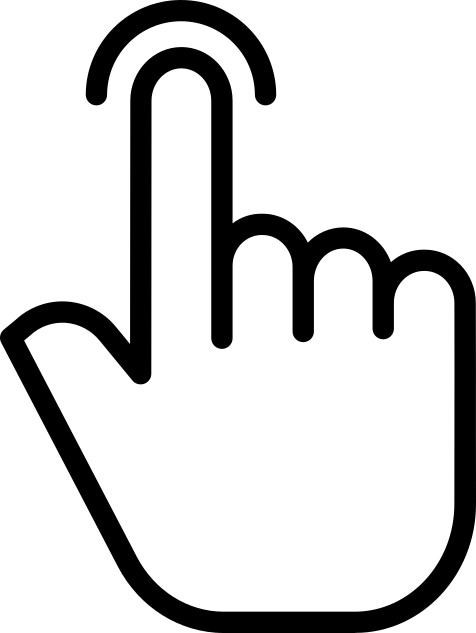
\includegraphics[width=0.03\textwidth]{static/dedo.png}} ;
         \node[factor, minimum size=1cm, xshift=3cm] (p3) {} ;
         
         \node[const, above=of p1, yshift=.15cm] (fp1) {$1/3$};
         \node[const, above=of p2, yshift=.15cm] (fp2) {$0$};
         \node[const, above=of p3, yshift=.15cm] (fp3) {$2/3$};
         \node[const, below=of p2, yshift=-.10cm, xshift=0.3cm] (dedo) {};
        } 
\end{figure}
  
Esta respuesta es diferente a la que obtuvimos con el primer modelo causal.
Sin embargo, ambas comparten la propiedad de ser la distribución de creencias que maximiza la incertidumbre dada la evidencia formal (modelo causal) y empírica (datos), lo que hace que sean proposiciones sobre las que podemos acordar tanto intercultural como intersubjetivamente.

\section{Reglas de la probabilidad}

Las reglas de la probabilidad han sido derivadas formalmente a partir de una gran cantidad de sistemas axiomáticos conceptualmente distintos e independientes entre si, lo cual es uno de los punto fuertes a su favor.
Pero quizás más importante es que ellas garantizan maximizar la incertidumbre dada la información empírica (datos) y formal (modelos causales).

% Parrafo

La teoría de la probabilidad tiene sólo dos reglas, conocidas como la regla de la suma y la regla del producto.
La primera regla computa la creencia de una variable simplemente como el total que ya le fue asignado en la creencia conjunta.
\begin{equation}
P(r_i) = \sum_j P(r_i, s_j)
\end{equation}
La segunda regla simplemente se queda con nueva creencia total a la creencia a priori que es compatible con el dato.
Expresada como producto
\begin{equation}
P(s_j)P(r_i|s_j) = P(r_i, s_j)
\end{equation}

Toda la teoría de la probabilidad se reduce a estas dos reglas.

\subsection{Teorema de Bayes}

El teorema de Bayes no es más que un corolario de las reglas de las probabilidad.

\begin{equation}
\begin{split}
P(r_i|s_2) = \frac{P(r_i, s_2)}{P(s_2)} = \frac{P(s_2|r_i)P(r_i)}{P(s_2)} 
\end{split}
\end{equation}

En términos más generales, $r_i$ representa las hipótesis y $s_2$ representa el dato.

\begin{equation*}
\underbrace{P(\text{Hip\'otesis }|\text{ Datos})}_{\text{\scriptsize Posteriori}} = \frac{\overbrace{P(\text{Datos }|\text{ Hip\'otesis})}^{\text{\scriptsize Verosimilitud}} \overbrace{P(\text{Hip\'otesis})}^{\text{\scriptsize Priori}} }{\underbrace{P(\text{Datos})}_{\text{\scriptsize Evidencia}}}
\end{equation*}

Es importante notar que todas estas probabilidades en realidad dependen de un cierto modelo causal, por lo correcto sería incluirlo explícitamente en el condicional.


\begin{equation*}
\underbrace{P(\text{Hip\'otesis }|\text{ Datos, Modelo})}_{\text{\scriptsize Posteriori}} = \frac{\overbrace{P(\text{Datos }|\text{ Hip\'otesis, Modelo})}^{\text{\scriptsize Verosimilitud}} \overbrace{P(\text{Hip\'otesis }|\text{ Modelo})}^{\text{\scriptsize Priori}} }{\underbrace{P(\text{Datos }|\text{ Modelo})}_{\text{\scriptsize Evidencia}}}
\end{equation*}

\subsection{Verosimilitud}

La verosimilitud es la predicción de los datos dada las hipótesis.
Veamos cuál es la verosimilitud, $P(s2|r_i)$, en el modelo de Monty Hall.

\begin{figure}[H]
\centering
\tikz{
\phantom{\node[latent, draw=white, yshift=0.8cm] (b0) {$1$};}
\node[latent,below=of b0,yshift=0.8cm, xshift=-3cm] (r1) {$r_1$};
\node[latent,below=of b0,yshift=0.8cm] (r2) {$r_2$};
\node[latent,below=of b0,yshift=0.8cm, xshift=3cm] (r3) {$r_3$};

\node[latent, below=of r1, draw=white, yshift=0.8cm] (br1) {$1$};
\node[latent, below=of r2, draw=white, yshift=0.8cm] (br2) {$1$};
\node[latent, below=of r3, draw=white, yshift=0.8cm] (br3) {$1$};
\node[latent,below=of br1,yshift=0.8cm] (c11) {$c_1$};
\node[latent,below=of br2,yshift=0.8cm] (c12) {$c_1$};
\node[latent,below=of br3,yshift=0.8cm] (c13) {$c_1$};

\node[latent, below=of c11, draw=white, yshift=0.8cm] (bc11) {$1$};
\node[latent, below=of c12, draw=white, yshift=0.8cm] (bc12) {$1$};
\node[latent, below=of c13, draw=white, yshift=0.8cm] (bc13) {$1$};
\node[latent,below=of bc11,yshift=0.8cm, xshift=-0.7cm] (r1d2) {$s_2$};
\node[latent,below=of bc11,yshift=0.8cm, xshift=0.7cm] (r1d3) {$s_3$};
\node[latent,below=of bc12,yshift=0.8cm] (r2d3) {$s_3$};
\node[latent,below=of bc13,yshift=0.8cm] (r3d2) {$s_2$};

\node[latent,below=of r1d2,yshift=0.8cm,draw=white] (br1d2) {$\frac{1}{2}$};
\node[latent,below=of r1d3,yshift=0.8cm, draw=white] (br1d3) {$\frac{1}{2}$};
\node[latent,below=of r2d3,yshift=0.8cm,draw=white] (br2d3) {$1$};
\node[latent,below=of r3d2,yshift=0.8cm,draw=white] (br3d2) {$1$};
\phantom{\edge[-] {b0} {r1,r2,r3};}
\edge[-] {r1} {br1};
\edge[-] {r2} {br2};
\edge[-] {r3} {br3};
\edge[-] {br1} {c11};
\edge[-] {br2} {c12};
\edge[-] {br3} {c13};
\edge[-] {c11} {bc11};
\edge[-] {c12} {bc12};
\edge[-] {c13} {bc13};
\edge[-] {bc11} {r1d2,r1d3};
\edge[-] {bc12} {r2d3};
\edge[-] {bc13} {r3d2};
\edge[-] {r1d2} {br1d2};
\edge[-] {r1d3} {br1d3};
\edge[-] {r2d3} {br2d3};
\edge[-] {r3d2} {br3d2};
}
\end{figure}

\begin{table}[H]
\centering
 $P(s_2|r_i)$   
 
 \begin{tabular}{c|c|c|c} \setlength\tabcolsep{0.4cm} 
          & \, $r_1$ \, &  \, $r_2$ \, & \, $r_3$ \, \\ \hline 
   $s_2$ & $1/2$ & $0$ & $1$  \\ \hline
\end{tabular}
\end{table}

\subsection{Posterior}

\subsection{Evidencia}




\section{Selección de modelos}


\chapter{Sistemas naturales de procesamiento de información}

En el último tercio de la historia del Universo, en algún momento hace aproximadamente 4500 millones de años, apareció en la tierra una forma de organización de la materia capaz de auto-replicarse.
El crecimiento de estos linajes siguieron procesos multiplicativos ruidosos: secuencias de probabilidades de supervivencia y reproducción.
Los errores producidos durante la replicación diversificaron las formas de vida, y las tasas de crecimiento de las diferentes estrategias favorecieron a aquellas mejor adaptadas al ambiente.
Desde aquel momento hasta ahora la vida adquirió una extraordinaria complejidad.
%
\begin{figure}[H]
    \centering
    \begin{subfigure}[b]{0.65\textwidth}
    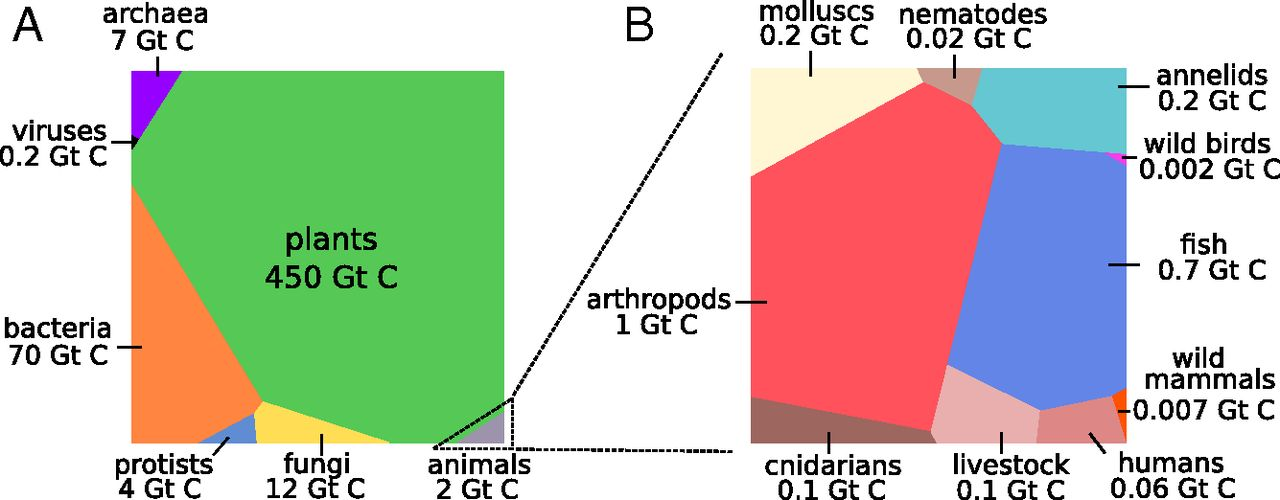
\includegraphics[width=\linewidth]{static/biomass.jpg}
    \end{subfigure}
    \caption{
	Estimación de la distribución actual de la biomasa en la tierra realizada por Bar-On~\cite{barOn2018-biomass}.
    }
    \label{fig:cpr_individual}
\end{figure}
%
Esta complejidad es consecuencia de una serie de transiciones evolutivas~\cite{maynardSmith1995-majorTransitions} en las que las entidades capaces de replicarse de forma independiente, cediendo algo de valor a las otras, pasan a formar unidades evolutivas de nivel superior.
Algunos ejemplos paradigmáticos son la transición de las moléculas replicantes a las protocélulas, la endosimbiosis de las mitocondrias y los plastos por parte de las células eucariotas, la aparición de los organismos multicelulares.
¿Cómo se explica esta tendencia permanente de la vida en favor de la agregación cooperativa?

\section{Evolución}

En evolución, el crecimiento de una estrategia $e$ en el tiempo, $\omega_e(t)$, esta gobernado por una secuencias estocástica de tasas de supervivencia y reproducción $f_e(\cdot)$ dependientes de un ambiente aleatorio $a$,
%
\begin{equation} \label{eq:modelo_exponencial}
\omega_e(T) = \prod_t^T f_e(a(t))
\end{equation}
%
donde $a(t)$ representa el estado del ambiente en el tiempo $t$.
Supongamos que la naturaleza lanza una moneda,
\begin{equation} \label{eq:estrategia_base}
f_e(a) =
\begin{cases}
 1.5 & a = \text{ Cara } \\
 0.6 & a = \text{ Seca }
\end{cases}
\end{equation}
Si sale cara la población se reproduce un 50\% y si sale seca sobrevive el 60\%.

% Parrafo

Según el modelo estándar de evolución, conocido como \emph{replicator dynamic} \cite{taylor1978-replicatorDynamic, schuster1983-replicatorDynamics, hofbauer2003-evolutionaryGameDynamics}, el cambio de la proporción de una estrategia $e$ en la población, $x_e$, está determinado por su tasa de crecimiento caracterísitica $f_e$,
\begin{equation} \label{eq:replicator_dynamic}
x_e^\prime = \frac{x_e f_e}{X}
\end{equation}
donde $X=\sum_i x_i f_i$ es el tamaño total de la población y actúa como constante de normalización.
¿Pero cuál es la tasa de crecimiento característica, $f_e$?
Su estimación requiere considerar explícitamente la variablidad del ambiente, $a$, y el tipo de proceso que genera esa variabilidad.

% Parrafo

Buena parte de la literatura en evolución considera que la estimación correcta se obtiene mediante el valor esperado de los recursos en el tiempo, $\omega_e(t)$.
Sea $\Omega_t$ el valor en el tiempo $t$ de todas las posibles trayectorias, su valor esperado se obtiene pesando cada estado $\omega_e \in \Omega_t$ por la probabilidad de que ocurra $P(\omega)$
%
\begin{equation}
\langle \omega_e \rangle_t = \sum_{\omega \in \Omega_t} \omega \cdot  P(\omega)
\end{equation}
%
El valor esperado en los dos primeros pasos temporales es, 
%
\begin{equation}
\begin{split}
\langle \omega_e \rangle_1 & = 1.5 \cdot \frac{1}{2} + 0.6 \cdot  \frac{1}{2} = 1.05 \\ 
\langle \omega_e \rangle_2 &=  1.5^2 \cdot \frac{1}{4} + 2 (0.6 \cdot 1.5 \cdot \frac{1}{4} ) + 0.6^2 \cdot \frac{1}{4}= 1.05^2
\end{split}
\end{equation}
%
Es decir, la tasa de crecimiento estimada según el valor esperado es de $5\%$ por cada paso temporal, $\langle \omega \rangle_t = 1.05^t$.
Y efectivamente eso es lo que ocurre con el promedio de las trayectoria individuales, $\omega_e(t)$, cuando la población es suficientemente grande,
%
\begin{figure}[H]
    \centering
    \begin{subfigure}[b]{0.45\textwidth}
    \includegraphics[width=\linewidth]{figures/pdf/ergodicity_expectedValue.pdf}
    \end{subfigure}
    \caption{
    Promedio de los recursos individuales en el tiempo para diferentes tamaños de la población, en escala logarítimica ($10^0,10^1,10^2,10^3,10^4$).
    A medida que aumentamos el tamaño de la población, el promedio se acerca al valor esperado $\langle \omega_e \rangle_t = 1.05^t$.
    }
    \label{fig:ergodicity_expectedValue}
\end{figure}

Sin embargo, el valor esperado no representa lo que lo le ocurre a los agentes en el tiempo. 
Individualmente, todas las trayectorias pierden a largo plazo a una tasa cercana al 5\%.
\begin{figure}[H]
    \centering
    \begin{subfigure}[b]{0.45\textwidth}
    \includegraphics[width=\linewidth]{figures/pdf/ergodicity_individual_trayectories.pdf}
    \caption{}
    \label{fig:ergodicity_individual_trayectories}
    \end{subfigure}
    \begin{subfigure}[b]{0.45\textwidth}
    \includegraphics[width=\linewidth]{figures/pdf/ergodicity_individual_trayectories_longrun.pdf}
    \caption{}
    \label{fig:ergodicity_individual_trayectories_longrun}
    \end{subfigure}
    \caption{
    La recta negra representan el valor esperado.
    Figura \ref{fig:ergodicity_individual_trayectories}: tamaño de los recursos individuales en el tiempo, $ \log(\omega_e(t))$.
    Figura \ref{fig:ergodicity_individual_trayectories_longrun}: con suficiente tiempo todas las trayectorias individuales se pegan a la recta azul. 
    }
    \label{fig:cpr_individual}
\end{figure}

La diferencia entre el valor esperado y lo que le ocurre a los agentes individuales en el tiempo es un problema bien conocido en mecánica estadística, llamado ``no-ergodicidad''~\cite{peters2019-ergodicityEconomics}.
Cuando un proceso es ergódico, las descripciones de su dinámica pueden remplazarse mediante el valor esperado, eliminado el tiempo de los modelos.
Sin embargo, las condiciones para que un sistema cumpla con la hipótesis de ergodicidad son muy restrictivas.
Cuando estas hipótesis no se cumplen nos vemos obligados a analizar directamente su dinámica. 

La dinámica evolutiva está gobernada por un procesos multiplicativos (eq.~\ref{eq:modelo_exponencial}), que en un cierto tiempo $t$ puede expresarse como,
\begin{equation}
\omega_e(T) = \prod^T_{t} f_e(a(t)) = f(\text{cara})^{n_1} f(\text{seca})^{n_2}
\end{equation}

donde $n_1$ y $n_2$ representa la cantidad de ocurrencias de $f_e(\text{cara})$ y $f_e(\text{seca})$, con $n_1 + n_2 = T$.
Las trayectorias observadas en la figura \ref{fig:ergodicity_individual_trayectories} son variables, pero cuanto más tiempo observemos el sistema más suave se vuelven esas líneas (figura \ref{fig:ergodicity_individual_trayectories_longrun}).
En el límite, $T \rightarrow \infty$ todas las trayectorias individuales estarán determinadas por la misma tasa de crecimiento $\overline{f_e}$ por el que se multiplica los recursos $\omega_e(T)$ en cada iteración.
\begin{equation}
\begin{split}
\lim_{T \rightarrow \infty} \omega_e(T) & = \overline{f_e}^T \\
\left( \lim_{T \rightarrow \infty} \omega_e(T) \right)^{1/T} & =  \overline{f_e} \\
\lim_{T \rightarrow \infty} f_e(\text{cara})^{n_1/T} f_e(\text{seca})^{n_2/T} & 
 \end{split}
\end{equation}
Donde las frecuencias $\frac{n_1}{T}$ y $\frac{n_2}{T}$ en el límite $T \rightarrow \infty$ son iguales a las probabilidades de ocurrencia de los estados del sistema.
Por lo tanto, la mejor estimación de la tasa de crecimiento es,
\begin{equation}
\overline{f_e} = (1.5 \cdot 0.6)^{1/2} \approx 0.95
\end{equation}


Esta fórmula, que permite computar la tasa de crecimiento caracterísitica a largo plazo de las trayectorias individuales surgidas de procesos multiplicativos, se la conoce también como \emph{media geométrica} y ha sido usada previamente en la literatura de evolución~\cite{dempster1955-geometricMean}.
Una propiedad importante es que su valor siempre es menor que el promedio de estados.
Esto se debe a que en los procesos multiplicativos los impactos físicos de las pérdidas suelen ser más fuertes que los de las ganancias.
En el extremo, un único cero en la productoria alcanza para generar su extinción.

% Decimos que un proceso es ergódico si se cumple que,
% \begin{equation}
%  \underbrace{\lim_{T \mapsto \infty} \frac{1}{T} \sum_{t=1}^T \omega(t)}_{\text{Media temporal}}  = \underbrace{\sum_{\omega} \omega \cdot p(\omega)}_{\text{Media de estados}}
% \end{equation}
% 

\subsection{Ventaja de la cooperación}

En los procesos no-ergódicos, las fluctuaciones tienen un efecto negativo en la tasa de crecimiento individual a largo plazo, pero no en la tasa de crecimiento del valor esperado.
Dado que la varianza realmente importa, una forma eficaz de reducirla es compartir los riesgos~\cite{yaari2010-cooperationEvolution, peters2015-evolutionaryAdvantageOfCooperation}.
%Parafraseando a Den Boer~\cite{denBoer1968-spreadingRisk}, la  supervivencia de una población depende de la distribución del riesgo dentro de la población y entre las poblaciones de diferentes especies.
Ole Peters~\cite{peters2015-evolutionaryAdvantageOfCooperation} considera las consecuencias que tiene sobre la tasa de crecimiento de los agentes la distribución del riesgo de una estrategia cooperativa sencilla.
La estrategia consiste en repartir los recursos en partes iguales luego de cada iteración.

\begin{figure}[H]
\centering
\scalebox{0.75}{
\tikz{

    \node[latent, minimum size=2cm ] (x1_0) {$\omega_1(t)$} ;
    \node[latent, below=of x1_0, minimum size=2cm ] (x2_0) {$\omega_2(t)$} ;

    \node[latent, right=of x1_0, minimum size=3cm ] (x1_0g) {$ \omega_1(t)\cdot f_e(a_1(t))$} ;
    \node[latent, right=of x2_0, minimum size=1.8cm, xshift=0.6cm , align=left] (x2_0g) {$\omega_2(t)\cdot$\\$f_e(a_2(t))$} ;
    
    \node[latent, right=of x1_0g, minimum size=3.8cm, yshift=-1.33cm, align=right] (x_0) {$\omega_1(t)\cdot f_e(a_1(t))$\\$+\omega_2(t)\cdot f_e(a_2(t))$ } ;
    
    \node[const, above=of x_0] (nx_0) {$\overbrace{\text{Pool}\hspace{2.5cm}\text{Share}}^{\text{\normalsize Cooperaci\'on}}$} ;
    
    \node[latent, right=of x1_0g, minimum size=2.5cm,  xshift=4.5cm] (x1_1) {$\omega_1(t+1)$ } ;
    \node[latent, below=of x1_1, minimum size=2.5cm, yshift=0.7cm] (x2_1) {$\omega_2(t+1)$ } ;
    
    \edge {x1_0} {x1_0g};
    \edge {x2_0} {x2_0g};
    \edge {x1_0g,x2_0g} {x_0};
    \edge {x_0} {x1_1,x2_1};
    
}
}
\caption{Estrategia cooperativa. Los agentes comienzan con los mismos recursos iniciales. Luego crecen independientemente de acuerdo con la ecuaci\'on \ref{eq:estrategia_base}. Luego cooperan poniendo sus recursos en un fondo común, que finalmente es dividio en partes iguales.}
\label{fig:protocolo}
\end{figure}

Las poblaciones enteramente cooperadoras reducen sus fluctuaciones, lo que genera una aumento en la tasa de crecimiento de todos sus miembros.
En la figura \ref{fig:cpr_absolute_cooperation} mostramos la trayectoria de uno de los agentes cooperadores.

\begin{figure}[H]
    \centering
    \begin{subfigure}[b]{0.45\textwidth}
    \includegraphics[width=\linewidth]{figures/cpr_absolute_cooperation.pdf}
    \end{subfigure}
    \caption{
    Tamaño logarítimico de los recursos de un individuo de una población con 33 agentes que comparten su riqueza luego de cada iteración.
    La recta negra que baja representa el promedio temporal, y la que sube el promedio de estados.
    }
    \label{fig:cpr_absolute_cooperation}
\end{figure}

Mediante la cooperación, las poblaciones de agentes logran acceder a tasas de crecimiento individuales equivalentes al promedio de estados del sistema, que en los sistemas no-ergódicos es siempre superior que el promedio temporal.

% Parrafo

Ole Peters considera que este aumento de la tasa de crecimiento demuestra la ventaja evolutiva de la cooperación, lo que propone como principal explicación de las transiciones evolutivas.
Sin embargo Ole Peters no analiza el problema de la deserción, quien dice ``our cooperators are unable to break the cooperative pact''.
No parece ser un problema menor, teniendo en cuenta la tentación que podría significar dejar de aportar al fondo común mientras se siguen recibiendo los beneficios de este.

\subsection{Transiciones evolutivas}

\todo[inline]{subsección no terminada}

Para discutir este punto en detalle, analizamos las tasas de crecimiento de las estrategias cooperadora y desertora en un caso concreto.


\begin{figure}[H]
    \centering
    \begin{subfigure}[b]{0.45\textwidth}
    \includegraphics[width=\linewidth]{figures/cpr_absolute_cooperation_defection_costo.png}
    \end{subfigure}
    \caption{
    Población de 100 agentes, a) totalmente cooperadores, b) con un desertor, c) con 10 desertores.
    }
    \label{fig:cpr_absolute_cooperation_defection_costo}
\end{figure}

Las estrategias desertoras, al evitar compartir sus recursos generan un aumento en sus propias fluctuaciones, afectando su tasa de crecimiento a largo plazo sin necesidad de introducir castigos.
Esto parecería apoyar la idea de Ole Peters de que la cooperación no es altruista sino que está impulsada por el interés personal.
Sin embargo, los agentes evolutivos no son agentes económicos, su frecuencia cambia en base a tasa de \emph{diferencial} de crecimiento.
Por más que la mutua cooperación sea mejor en términos absolutos, un mutante desertor tendrá una tasa de crecimiento mayor a la de su comañero cooperador, por lo que invadirá evolutivamente la población. 

\section{La transición cultural}

Antes del surgimiento de los humanos \emph{anatómicamente} modernos (masa cerebral actual) y de los humanos \emph{conductualmente} modernos (lenguaje), surgió en África una linaje \emph{emocionalmente} moderno~\cite{hrdy2020-emotionallyModern}, capaz de leer las intenciones de los otros.
La especial integraci\'on de los procesos biol\'ogicos, cognitivos y sociales que permite a los humanos desarrollar culturas complejas se debió a una coevolución genético-cultural desencadenada por el surgimiento previo de la crianza cooperativa~\cite{hrdy2020-emotionallyModern}.
La forma en la que estos homininos organizaron la crianza produjo un ambiente que favoreció la selección de jóvenes capaces de monitorear y comprender las intenciones de los demás, y de atraer la atención de sus cuidadadores de modo de compartir sus propias necesidades.

% Parrafo

La empatía fue la habilidad que permitió el desarrollo del Homo sapiens.
Esta costosa habilidad cognitiva es especialmente eficiente para la adquisición de tradiciones complejas: la comprensión mutua, la imitación y el lenguaje
Lo que antes debía ser redescubierto una y otra vez mediante costosa experiencia individual, ahora podía ser transmitido a la siguiente generación.
La capacidad de adquirir comportamientos basados en la experiencia de otros sin tener que re-construirlos cada vez por prueba y error conduce un proceso de evolución y acumulativa cultural que permite a las poblaciones humanas adaptarse rápidamente ante cambios bruscos en el ambiente o migraciones a nuevos entornos.

% Parrafo

El surgimiento de la cultura produjo cambios radicales para nuestra especie.
Antes de la transición cultural, estuvimos en grave peligro de extinción, lo que se evidencia en la baja diversidad del genoma humano.
Luego de la transición cultural, en pocos años nuestra especie ocupó todos los nichos ecológicos de la tierra como ningún otro vertebrado terrestre lo había logrado antes.
Esta proeza se logró mediante los sistemas culturales y tecnológico desarrollados por sociedades cazadores-recolectores.
Caminando salimos de África, ocupamos Asia, y de allí Oceanía y las Américas (las flechas del mapa~\ref{fig:agricultura}).
La información transgeneracional fue la que le permitió a estas sociedades simples adaptarse rápidamente a los nuevos desafíos ecológicos.

% Parrafo

El cambio climático ocurrido al inicio del Holoceno (hace 12000 años) propició el desarrollo de la agricultura, que surgió de manera independiente en los seis grandes sistemas geográficos de la tierra: en la región central de África subsahariana, en Asia occidental, en Asia oriental, en Oceanía norte, en América del norte y en América del sur (las puntos rojos del mapa~\ref{fig:agricultura}).
\begin{figure}[H]
    \centering
    \begin{subfigure}[b]{0.6\textwidth}
     \includegraphics[width=\textwidth]{figures/agricultura.pdf}
     \label{fig:agricultura}
    \end{subfigure}
%     \begin{subfigure}[b]{0.40\textwidth}
%     \includegraphics[width=\textwidth]{static/polynesia.png} 
%     \caption{Poblamiento del océano Pacífico}
%     \label{fig:polynesia}
%     \end{subfigure}
    \caption{
    Proyección políedrica de la tierra que conserva los tamaños relativos de los continentes.
    Las felchas indican el poblamiento, desde África a Asia, y de Asia hacia Oceanía y América.
    Los puntos rojos indican surgimiento independiente de agricultura.
    }%
    \label{fig:poblamiento}
\end{figure}
%
Alrededor de estos puntos se desarrollaron los principales centros poblacionales de la humanidad.
El aumento de la población promovió, a su vez, el desarrollo de nuevas innovaciones tecnológicas y científicas, como la escritura, la matem\'aticas, las ingenier\'ias, la astronomía, las ciencias políticas, entre otras.
Durante el año 1400 el mundo florecía de sociedades "prósperas"~\cite{dussel2004-sistemaMundo}: Aztecas en Ámerica del norte, Incas en Ámerica del sur, Tongas en el Pacífico, Bantúes en África sub-sahariana, los Árabes e Indios en Asia occidental y Chinos en Asia oriental, por mencionar algunos.

\subsection{Evolución cultural}

La especie humana posee la peculiar capacidad de desarrollar innovaciones culturales a lo largo de m\'ultiples generaciones, un fen\'omeno denominado \emph{evoluci\'on cultural acumulada}~\cite{Derex2020} (o \textbf{CCE} por sus siglas en ingl\'es).
El modelo causal b\'asico de la literatura de evoluci\'on cultural afirma que la adaptaci\'on humana depende, adem\'as de la experiencia individual y los cambios en el ambiente, de la informaci\'on cultural a la que tienen acceso los agentes.

\begin{figure}[H]
	\centering
	\tikz{
    	\node[accion] (a) {} ;
	    \node[const,below=of a] (na) {Adaptaci\'on} ;
	    \node[accion,above=of a, xshift=-0.8cm] (e) {} ;
	    \node[const,left=of e] (ne) {Experiencia} ;
	    \node[accion,above=of a, xshift=0.8cm] (s) {} ;
	    \node[const,right=of s] (ns) {Informaci\'on cultural} ;
	    \node[accion,above=of a, yshift=0.6 cm] (m) {} ;
	    \node[const,above=of m] (nm) {Medio ambiente} ;
	    \edge {e,s,m} {a};
	}
	\caption{Representaci\'on gr\'afica de un modelo causal para la adaptaci\'on humana.}
\end{figure}

Todas las tecnolog\'ias surgen como resultado de esfuerzo transgeneracionales.
Basada en los principios b\'asicos de la teor\'ia evolutiva (descendencia, modificaci\'on y selecci\'on), la antropolog\'ia ha desarrollado un marco te\'orico para explicar c\'omo cambia la cultura en el tiempo.
Este marco ha motivado el desarrollo de los primeros modelos matem\'aticos para explicar distintas din\'amicas poblacionales de producci\'on, transmisi\'on y mantenimiento de informaci\'on cultural~\cite{cavalliSforza1981-culturalTransmission,boyd1985-evolutionaryProcess}.

% Parrafo

Una idea central en estos trabajos es que el aprendizaje social (por imitaci\'on, observaci\'on, etc.) no es al azar, sino que los individuos eligen de qui\'en aprender.
Por ejemplo, una estrategia simple consiste en copiar lo que hace la mayor\'ia (\emph{frequency-based strategy}).
Otra estrategia t\'ipica toma como modelo de referencia a las personas m\'as exitosas o prestigiosas (\emph{payoff-based strategy}). %, y llama a los individuos exitosos (de los cuales otros individuos aprenden) \textbf{demostradores}.
Las diferentes estrategias de aprendizaje social que se han propuesto~\cite{rendell2010-socialLearningTournament} pueden ser clasificadas entre aquellas que identifican de qui\'enes aprenden los individuos, y aquellas que especifican las circunstancias bajo las cuales los individuos copian a otros.
Por ejemplo, mantener compa\~neros de equipo estable est\'a relacionado con un mayor aprendizaje~\cite{Landfried2019}.

\todo[inline]{Subsección no terminada}

% Parrafo

\section{Objetivos}

\todo[inline]{Sección objetivos}

\chapter{TrueSkill Through Time}

\section{Introducción}


Los humanos desarrollamos habilidades complejas gracias a una integraci\'on especial de los procesos biol\'ogicos, cognitivos y sociales~\cite{Koster2020}.
Nuestra extraordinaria capacidad para imitar, combinada con los largos per\'iodos de aprendizaje juvenil y vida posreproductiva, permite a los humanos aprender de los dem\'as y transmitir las innovaci\'on a trav\'es de la generaciones~\cite{Richerson2020}.
Al ser un proceso poblacional, la adaptaci\'on humana tambi\'en se ve afectada por caracter\'isticas demogr\'aficas, como el tama\~no y estructura de las poblaciones~\cite{Derex2020}.

%

Conocer c\'omo cambian las habilidades individuales a lo largo del tiempo es esencial en el sistema educativo y laboral.
Dado que son variables ocultas, lo mejor que podemos hacer es estimarlas a partir de sus consecuencias observables directas: el producto de la resoluci\'on de problemas y competencias.
Sin embargo la estimación de curvas de aprendiaje es tema sensible, especialmente cuando se las pretende utilizar para tomar decisiones que pueden impactar a las personas.
Considerar s\'olo la frecuencia de resultados positivos como indicador de la habilidad de los individuos puede conducir a aproximaciones erroneas, fundamentalmente porque su valor depende tambi\'en de la dificultad de los desaf\'ios.
Por esta raz\'on, todos los estimadores de habilidad ampliamente usados se basan en comparaciones por pares.
Desde los primeros modelos generativos, propuestos hace casi un siglo por~\cite{Thurstone1927} y~\cite{Zermelo1929}, se supone que la probabilidad de un resultado observado $r$ depende del rendimiento $p$ del agente $i$ y de su oponente $j$, expresada como $P(\, r \,|\, p_i, \, p_j \,)$.
El campo sigui\'o progresando con los trabajos de \cite{Bradley1952} y~\cite{Mosteller1951a,Mosteller1951b,Mosteller1951c}, que condujeron al gran avance que tuvo lugar cuando~\cite{Elo2008} desarrolló una metodología para la Federaci\'on de Ajedrez de los Estados Unidos (USCF), adoptada hasta el d\'ia de hoy por la Federaci\'on Internacional de Ajedrez (FIDE).

% Parrafo

Todos los estimadores de habilidad ampliamente utilizados en la actualidad comparten alguna variante del modelo probabil\'istico propuesto por Elo~\cite{Glickman1999, Herbrich2007, VanDerLinden2016, Fox2010}.
%
\begin{figure}[ht!]
\centering \small
    \tikz{         
    \node[det, fill=black!10] (r) {$r$} ; 
    \node[const, left=of r, xshift=-1.35cm] (r_name) {\small \en{Result}\es{Resultado}:}; 
    \node[const, right=of r] (dr) {\normalsize $ r = (d > 0)$}; 

    \node[latent, above=of r, yshift=-0.45cm] (d) {$d$} ; %
    \node[const, right=of d] (dd) {\normalsize $ d = p_i-p_j$}; 
    \node[const, left=of d, xshift=-1.35cm] (d_name) {\small \en{Difference}\es{Diferencia}:};
    
    \node[latent, above=of d, xshift=-0.8cm, yshift=-0.45cm] (p1) {$p_i$} ; %
    \node[latent, above=of d, xshift=0.8cm, yshift=-0.45cm] (p2) {$p_j$} ; %
    \node[const, left=of p1, xshift=-0.55cm] (p_name) {\small \en{Performance}\es{Desempeño}:}; 

    \node[accion, above=of p1,yshift=0.3cm] (s1) {} ; %
    \node[const, right=of s1] (ds1) {$s_i$};
    \node[accion, above=of p2,yshift=0.3cm] (s2) {} ; %
    \node[const, right=of s2] (ds2) {$s_j$};
    
    \node[const, right=of p2] (dp2) {\normalsize $p \sim \N(s,\beta^2)$};

    \node[const, left=of s1, xshift=-.85cm] (s_name) {\small \en{Skill}\es{Habilidad}:}; 
    
    \edge {d} {r};
    \edge {p1,p2} {d};
    \edge {s1} {p1};
    \edge {s2} {p2};
    %\node[invisible, right=of p2, xshift=4.35cm] (s-dist) {};
}
     \caption{
    Modelo generativo en el que las habilidades causan los resultados observables a trav\'es de la diferencia de rendimientos ocultos, $d=p_i-p_j$, ambas variables aleatorias centradas en la verdadera habilidad, $p \sim \N(s,\beta^2)$.
    Quien haya obtenido mayor rendimiento gana, $r = (d > 0)$.
    Las variables observables se pintan de gris, las ocultas en blanco, y las constantes se muestran como puntos negros.
    }
    \label{fig:generative_model}
\end{figure}
La figura~\ref{fig:generative_model} ofrece un modelo causal en el que las habilidades generan el resultado observable.
Los agentes exhiben distintos desempe\~nos en cada evento, que var\'ian alrededor de su verdadera habilidad, $\N(p\,|\,s,\beta^2)$.
El modelo supone que gana el agente con mayor rendimiento, $r = (p_i > p_j)$. En otras palabras, gana quien obtenga una diferencia de desempeño mayor a 0, $r = (p_i - p_j > 0)$.
El parámetro $\beta^2$, al ser el mismo para todos los agentes, act\'ua como la escala de las estimaciones: habilidades separada por un $\beta$ mantienen siempre la misma probabilidad de ganar independiente del valor absoluto de las estimaciones.

% Parrafo

A partir de la representaci\'on gr\'afica propuesta en la figura \ref{fig:generative_model}, se puede derivar la predicci\'on del resultado dadas las estimaciones previas, $P(\,r\,|\,s_{i_\text{old}},s_{j_\text{old}}\,)$.
La soluci\'on metodol\'ogica de Elo es simple y astuta: actualizar las estimaciones previas, $s_{i_\text{old}}$ y $s_{j_\text{old}}$, en base a la sorpresa, i.e. el complemento de la predicci\'on del resultado observado.
%
\begin{equation} \label{eq:elo_delta}
 \Delta = \underbrace{\left(1-P(\,r\,|\,s_{i_\text{old}},s_{j_\text{old}}\,)\right)}_{\text{\en{Surprise}\es{Sorpresa}}}
\end{equation}
Donde la probabilidad surge de instanciar las estimaciones previas en el modelo generativo (detalles en la secci\'on~\ref{sec:2vs2}).
La idea es que la magnitud de la sorpresa $\Delta$ est\'a relacionada con cuan buenas son las estimaciones previas, y por lo tanto puede usarse para actualizarlas.
Resultados inesperados indicar\'ian que las estimaciones actuales no son del todo correctas y deber\'ian actualizarse en mayor medida que si hubieran ocurrido como se esperaba.
%
\begin{equation}\label{eq:elo_update}
 s_{\text{winner}_\text{new}} = s_{\text{winner}_\text{old}} + \Delta \ \ \ \ \ s_{\text{loser}_\text{new}} = s_{\text{loser}_\text{old}} - \Delta 
\end{equation}
Donde la sorpresa $\Delta$ act\'ua como factor de correcci\'on para ambas estimaciones previas.
Esta soluci\'on puede recuperar la escala relativa de los agentes, partiendo de valores iniciales arbitrarios.
Sin embargo, tiene algunas debilidades importantes.
La regla de actualizaci\'on (Ec.~\eqref{eq:elo_update}) es sim\'etrica, as\'i que lo que gana un agente el otro lo pierde.
Debido a que a los agentes nuevos comienzan con estimaciones arbitrarias (el mismo valor inicial para cualquier individuo), ellas tienden a generan alta sorpresa y por lo tanto pueden modificar bruscamente las estimaciones de sus oponentes a pesar de que ya hubieran convergido.
Esta debilidad ocurre por no tener en cuenta la incertidumbre sobre las estimaciones de los agentes.
Una soluci\'on ad-hoc fue propuesta para resolver este problema: reducir el impacto de la sorpresa en funci\'on de la cantidad de veces que el agente ha participado previamente.
% Ese es rol que desempe\~na el K-factor usado por la FIDE, $\Delta_i = \Delta \cdot K_i$.

% Parrafo

Una alternativa superadora consiste en distribuir nuestra creencia entre todas las posibles hipótesis de habilidad, en vez de seleccionar un \'unico valor como estimaci\'on.
Este enfoque conocido como inferencia bayesiana ha demostrado ser exitoso en la pr\'actica~\cite{Bishop2006} y garantiza un razonamiento consistente en contextos de incertidumbre~\cite{Jaynes2003,VanHorn2003}.
Toda inferencia de este tipo, no importa cuan compleja sea, puede ser resuelta mediante las reglas de la probabilidad: la~\ref{eq:sum_rule} y la~\ref{eq:product_rule}.
La \ref{eq:sum_rule} afirma que cualquier distribuci\'on marginal se puede obtener integrando o sumando la distribuci\'on conjunta.
%
\begin{equation} \label{eq:sum_rule}
 \tag{\en{sum rule}\es{regla de la suma}}
 P(x) = \sum_{y} P(x,y) \ \ \ \ \ \text{or} \ \ \ \ \ p(x) = \int p(x,y) \, dy
\end{equation}
Donde $P(\cdot)$ y $p(\cdot)$ representan distribuciones de probabilidad discretas y continuas respectivamente.
Adem\'as, la \ref{eq:product_rule} se\~nala que cualquier distribuci\'on conjunta puede ser expresada como el producto de distribuciones condicionales uni-dimensionles.
%
\begin{equation}\label{eq:product_rule}
\tag{\en{product rule}\es{regla del producto}}
 p(x,y) = p(x|y) p(y)
\end{equation}
%
\en{From these rules, we immediately obtain the~\ref{eq:bayes_theorem}:}
\es{De estas reglas obtenemos inmediatamente el~\ref{eq:bayes_theorem},}
%
\begin{equation}\label{eq:bayes_theorem}
\tag{\en{Bayes' theorem}\es{Teorema de bayes}}
 p(y|x) = \frac{p(x|y)p(y)}{p(x)}
\end{equation}
%
% 
% El uso inferencial del teorema de bayes juega un rol central en las t\'ecnicas modernas de aprendizaje estad\'isitico.
El \ref{eq:bayes_theorem} actualiza de forma \'optima las creencia sobre las hip\'otesis, maximizando la incertidumbre luego de haber incorporar la información provista por el modelo y los datos.
%
Para cuantificar la incertidumbre de nuestras hip\'otesis de habilidades utilizando la informaci\'on que nos ofrece el resultado observado y el modelo causal descrito, necesitamos resolver:
%
\begin{equation}\label{eq:event_inference} 
 \underbrace{p(\overbrace{\text{\en{Skill}\es{Habilidad}$_i$}}^{\text{\en{Hidden}\es{Oculta}}}|\overbrace{\text{Result\es{ado}}}^{\text{Observ\en{ed}\es{ado}}}, \text{Model\es{o}})}_{\text{Posterior}} = \frac{\overbrace{P(\,\text{Result\es{ado}}\,|\,\text{\en{Skill}\es{Habilidad}$_i$}\,,\text{Model\es{o}})}^{\text{\en{Likelihood}\es{Verosimilitud}}}\overbrace{p(\text{\en{Skill}\es{Habilidad}$_i$})}^{\text{Prior}}}{\underbrace{P(\text{Result\es{ado}}\,|\,\text{Model\es{o}})}_{\text{Evidenc\en{e}\es{ia} o\en{r}\es{ predicci\'on a} prior \en{prediction}}}}
\end{equation}
Donde la \'unica variable libre es la hip\'otesis de habilidad del agente $i$.
El prior cuantifica la incertidumbre sobre la habilidad antes de ver el resultado, y el posterior cuantifica la incertidumbre luego de ver el resultado.
La verosimilitud y la evidencia son ambas probabilidades del resultado observado, por lo que pueden ser vistas como predicciones.
Como los resultados son variables discretas, esas probabilidad se escribe con letras may\'usculas.
Debido a que la evidencia es la misma para todas las hip\'otesis, el \'unico factor que actualiza nuestras creencias es la verosimilitud.

% Parrafo

A modo de ejemplo, consideremos un caso ganador ($p_i > p_j$) usando priors gaussianos, $\N(\,s\,|\,\mu, \sigma^2)$.
Nuestra creencia a priori respecto de la diferencia de desempeños, $d=p_i-p_j$, se puede expresar como una gaussiana centrada en la diferencia de las medias de las estimaciones a priori ($\mu_i - \mu_j$), con una varianza que incorpora la incertidumbre de ambas estimaciones ($\sigma$) y la varianza de ambos rendimientos ($\beta$), $\N(\, d \, | \, \mu_i -\mu_j \, ,\ 2\beta^2 + \sigma_i^2 + \sigma_j^2 \,)$.
Al observar que el agente $i$ gan\'o, sabemos por el modelo causal que la diferencia de desempeños oculta fue en efecto positiva.
Por lo tanto, la predicci\'on a priori del resultado observado, o evidencia, es la densidad acumulada ($\Phi$) de todos los valores positivos de la gaussiana de diferencia de desempeños (Eq.~\eqref{eq:evidence}).
A partir de ahora el rol del modelo se dejr\'a impl\'icito.
%
\begin{equation}\label{eq:evidence}
 \overbrace{P(r)}^{\text{Evidenc\en{e}\es{ia}}} = 1-\Phi(0 \, | \overbrace{\mu_i^{\phantom{2}} - \mu_j}^{\hfrac{\text{\en{Expected}\es{Diferencia}}}{\text{\en{difference}\es{esperada}}}} , \, \overbrace{2\beta^2 + \sigma_i^2+ \sigma_j^2}^{\hfrac{\text{\en{Total}\es{Incertidumbre}}}{\text{\en{uncertainty}\es{total}}}})
\end{equation}
La evidencia es una predicci\'on hecha con todas las hip\'otesis a priori.
Como es constante, la incertidumbre a posteriori de cada hip\'otesis es proporcional al producto de su incertidumbre a priori y su verosimilitud, como se muestra en la ecuaci\'on~\eqref{eq:posterior_win}.
En la secci\'on~\ref{sec:2vs2} veremos en detalle c\'omo todas estas ecuaciones surge de aplicar las reglas de las suma y el producto sobre el modelo.
%
\begin{equation}\label{eq:posterior_win}
\underbrace{p(\,s_i\, | \, r \, )}_{\text{Posterior}} \propto \underbrace{1-\Phi(0 \, |  s_i - \mu_j , \, 2\beta^2 + \sigma_j^2)}_{\text{\en{Likelihood}\es{Verosimilitud}} \ P(r|s_i)} \,  \underbrace{\N(s_i \, | \, \mu_i,\, \sigma_i^2)}_{\text{Prior} \ p(s_i)} 
\end{equation}
Donde el posterior normalizado se obtiene dividiendo el lado derecho con la evidencia, $P(r)$.
Es interesante notar las similitudes y diferencias entre la verosimilitud y la evidencia.
La verosimilitud cuantifica la misma densidad acumulada que la evidencia, pero centrada ahora en la diferencia entre la hip\'otesis que estamos evaluando $s_i$ y la estimaci\'on media del oponente $\mu_j$, con una varianza que incluye todas las incertidumbres salvo la de la propia hip\'otesis $s_i$.
En otras palabras, la verosimilitud no es m\'as que la predicci\'on a priori del resultado observado suponiendo verdadera la hip\'otesis de habilidad que estamos evaluando.
La figura~\ref{fig:posterior_win} muestra en t\'erminos gr\'aficos el procedimiento de actualizaci\'on que realiza la ecuaci\'on~\eqref{eq:posterior_win}.
%
\begin{figure}[ht!]
    \centering
    \en{\includegraphics[page={1},width=.6\linewidth]{figures/posterior_win}}
    \es{\includegraphics[page={2},width=.6\linewidth]{figures/posterior_win}}
    \caption{
    Actualizaci\'on de creencias para el caso ganador.
    El posterior proporcional se obtiene como el producto de la distribuci\'on a priori (distribuci\'on gaussiana) y la verosimilitud (distribuci\'on gaussiana acumulada).
    La evidencia es la integral del posterior proporcional.
    Las distribuciones no est\'an necesariamente en la misma escala: la distribuci\'on a priori integra 1, mientras que la verosimilitud va de 0 a 1.
    }
    \label{fig:posterior_win}
\end{figure}

El posterior no es m\'as que la densidad del prior no filtrada por la verosimilitud.
La sorpresa, definida como el complemento de la verosimilitud, funciona como un filtro para el prior.
En la regi\'on de hip\'otesis de muy alta habilidad, donde el resultado ganador no nos hubiera generado casi ninguna sorpresa ($\lim_{s_i \to \infty}P(r|s_i) = 1$), el posterior recibe casi toda la densidad del prior.
En cambio, en la regi\'on de hip\'otesis de muy baja habilidad, donde el resultado habr\'ia generado mucha sorpresa ($\lim_{s_i \to -\infty}P(r|s_i) = 0$), el posterior no recibe casi nada de la densidad del prior.

% Parrafo

Es importante remarcar que la posterior, aunque se parezca, no es una distribuci\'on gaussiana, lo que nos impedir\'a usar la ecuaci\'on~\eqref{eq:posterior_win} iterativamente.
Por la forma del posterior exacto, una gaussiana puede ser usada como una buena aproximaci\'on, permiti\'endonos evitar el costo computacional de las metodolog\'ias de sampleo.
Uno de los principales aportes del sistema Glicko~\cite{Glikman2013} fue el desarroll\'o de un m\'etodo eficiente para aproximar la posterior exacta con una distribuci\'on gaussiana.
Sin embargo, este m\'etodo no garantiza que la distribuci\'on gaussiana seleccionada sea la que mejor aproxima.
El \'exito de la soluci\'on TrueSkill~\cite{Herbrich2007} se basa en la aplicaci\'on de m\'etodo eficiente para calcular la gaussiana que mejor aproxima al posterior exacto (secci\'on~\ref{sec:approximate_posterior}),
%
\begin{equation} \label{eq:approx} 
 \widehat{p}(s_i| r, s_j) = \underset{\mu, \sigma}{\text{ arg min }} \ \ \text{KL}(\, p(s_i| r, s_j) \, || \,  \N(s_i|\mu, \sigma^2) \, )
\end{equation}
en términos de minización de la divergencia Kullback-Leibler entre la distribuci\'on verdadera y la aproximada.
Este método nos permite aplicar eficientemente la ecuaci\'on~\eqref{eq:posterior_win} iterativamente sobre una secuencia de observaciones, que de otra manera sería inviable.
El enfoque adoptado por TrueSkill para tratar el proceso din\'amico, conocido como \emph{filtering}, usa el último posterior aproximado como prior del siguiente evento.
Luego, el posterior aproximado en un determinado momento se define como,
%
\begin{equation}\label{eq:filter} %\tag{\text{filtering}}
 \widehat{\text{Posterior}}_t \propto \widehat{\text{Likelihood}}_t  \overbrace{\widehat{\text{Likelihood}}_{t-1} \dots \underbrace{\widehat{\text{Likelihood}}_{1} \text{Prior}_1}_{\widehat{\text{Posterior}}_{1} \text{ \en{as}\es{como} } \text{Prior}_{2}} }^{\widehat{\text{Posterior}}_{t-1} \text{ \en{as}\es{como} } \text{Prior}_{t}} %= \text{Prior}_1 \prod_{i=1}^t \text{Likelihood}_i 
\end{equation}
Donde {\footnotesize $\widehat{\text{Posterior}}_i$} y {\footnotesize $\widehat{\text{Likelihood}}_i$} representan la aproximaciones inducidas por la ecuaci\'on~\eqref{eq:approx} en el $i$-\'esimo evento.
Si consideramos la verosimilitud como un filtro del prior, cada posterior puede ser visto como una acumulaci\'on de todos los filtros anteriores.
De esta forma, la informaci\'on propaga del estimaciones pasadas hacia futuras.
Debido a que las habilidades cambian en el tiempo, es importante agregar alguna incertidumbre $\gamma$ luego de cada paso.
%
\begin{equation}\label{eq:dynamic_factor}
 \widehat{p}(s_{i_t}) = \N(s_{i_t} | \mu_{i_{t-1}}, \sigma_{i_{t-1}}^2 + \gamma^2 )
 \end{equation}
Debido a que el enfoque de filtrado es un procedimiento ad-hoc que no surge de ningún modelo probabilístico, sus estimaciones exhiben una serie problemas.
El m\'as obvio es que el inicio de toda secuencia de estimaciones siempre tiene alta incertidumbre.
Pero tambi\'en se observan desacoplamientos temporales y espaciales que impiden comparar estimaciones: aunque la diferencias relativas entre estimaciones contempor\'aneas al interior de comunidades bien conectadas sean correctas, las estimaciones separadas en el tiempo y entre comunidades poco conectadas suelen ser incorrectas.
Todos estos problemas están relacionados al hecho de que la información propaga en una sola dirección a través del sistema, cuando la inferencia debería realizarse con toda la información disponible, también de eventos que ocurren de forma paralela como de eventos futuros disponibles.

% Parrafo

TrueSkill Through Time~\cite{Dangauthier2007} corrige los sesgos de los modelos previos mediante utilización de un único modelo probabilísitico para toda la historia de eventos.
Al estar teóricamente bien fundado podemos realizar la inferencia aplicando estrictamente las reglas de la probabilidad, lo que garantiza tanto buenas estimaciones iniciales como la comparabilidad temporal y espacial de las estimaciones.
Exluyendo el aspecto din\'amico, $\gamma = 0$, el prior de un agente $i$ en el $t$-\'esimo evento es el producto del todas sus verosimilitudes, salvo la del $t$-\'esimo evento.
%
\begin{equation}\label{eq:smooth_prior}
 \text{Prior}_{i_t} = \text{Prior}_{i_0} \underbrace{\prod_{k = 1}^{t-1} \text{\en{Likelihood}\es{Verosimilitud}}_{i_k}}_{\text{\en{Past information}\es{Informaci\'on pasada}}} \underbrace{\prod_{k = t + 1}^{T_i} \text{\en{Likelihood}\es{Verosimilitud}}_{i_k}}_{\text{\en{Future information}\es{Informaci\'on futura}}}
\end{equation}
Donde $T_i$ es la cantidad total de eventos del agente $i$, siendo {\small Prior$_{i_0}$} su prior inicial.
La conectividad entre eventos surge de suponer que la habilidad de un jugador en un tiempo $t$ depende de su propia habilidad en un tiempo anterior $t-1$, generando un red que adquiere su estructura dependiendo de quienes participan en cada evento.
Algoritmos similares fueron implementados por \cite{Coulom2008} y \cite{Maystre2019} basados en aproximaciones laplacianas y procesos gaussianos respectivamente.
Esto produce una mutua dependencia entre estimaciones que nos obliga a usar iterativamente las últimas verosimilitudes disponibles hasta alcanzar convergencia (detalles en la secci\'on~\ref{sec:throughTime}).
%
\begin{figure}[ht!]
  \centering
  \scalebox{.9}{
    \tikz{ %
      \node[latent] (s10) {$s_{a_0}$} ;
      %
      \node[latent,  below=of s10,yshift=-0.7cm] (s11) {$s_{a_1}$} ;
      
      \node[latent, right=of s11, xshift=3cm] (p11) {$p_{a_1}$} ;
      %
      \node[latent, below=of s11,yshift=-0.4cm] (s12) {$s_{a_2}$} ;
      \node[latent, right=of s12, xshift=3cm] (p12) {$p_{a_2}$} ;
      
      \node[const, right=of p11,xshift=0.5cm] (r1) {$\bm{>}$} ;
      \node[const, above=of r1, yshift=0.3cm] (nr1) {\footnotesize \ \  Observed result} ;
      \node[const, right=of p12,xshift=0.5cm] (r2) {$\bm{<}$} ;
      \node[const, above=of r2, yshift=0.3cm] (nr2) {\footnotesize \ \ Observed result} ;
      
      \node[latent, left=of s10, xshift=13.4cm] (s20) {$s_{b_0}$} ;
      \node[latent, below=of s20,yshift=-0.7cm] (s21) {$s_{b_1}$} ;
      \node[latent, left=of s21, xshift=-3cm] (p21) {$p_{b_1}$} ;
      
      \node[latent, below=of s21, yshift=-0.4cm] (s22) {$s_{b_2}$} ;
      \node[latent, left=of s22, xshift=-3cm] (p22) {$p_{b_2}$} ;
      
      
      \edge {s10} {s11};
      \edge {s11} {s12};
      \edge {s20} {s21};
      \edge {s21} {s22};
      \edge {s11} {p11};
      \edge {s12} {p12};
      \edge {s21} {p21};
      \edge {s22} {p22};
      
      \node[const, right=of s10, yshift=0cm ] (wp10) {\includegraphics[page={13},width=.125\linewidth]{figures/smoothing}} ;
      \node[const, left=of s20, yshift=0cm ] (wp20) {\includegraphics[page={13},width=.125\linewidth]{figures/smoothing}} ;
      
      
      \node[const, left=of s11, yshift=0.6cm ] (post11) {\includegraphics[page={1},width=.125\linewidth]{figures/smoothing}} ;
      \node[const, right=of s11, yshift=0.6cm ] (wp11) {\includegraphics[page={2},width=.125\linewidth]{figures/smoothing}} ;
      \node[const, left=of p11, yshift=0.6cm ] (lh11) {\includegraphics[page={3},width=.125\linewidth]{figures/smoothing}} ;
      
      \node[const, left=of s12, yshift=0.6cm ] (post12) {\includegraphics[page={4},width=.125\linewidth]{figures/smoothing}} ;
      \node[const, right=of s12, yshift=0.6cm ] (wp12) {\includegraphics[page={5},width=.125\linewidth]{figures/smoothing}} ;
      \node[const, left=of p12, yshift=0.6cm ] (lh12) {\includegraphics[page={6},width=.125\linewidth]{figures/smoothing}} ;
      
      
      \node[const, right=of s21, yshift=0.6cm ] (post21) {\includegraphics[page={7},width=.125\linewidth]{figures/smoothing}} ;
      \node[const, left=of s21, yshift=0.6cm ] (wp21) {\includegraphics[page={8},width=.125\linewidth]{figures/smoothing}} ;
      \node[const, right=of p21, yshift=0.6cm ] (lh21) {\includegraphics[page={9},width=.125\linewidth]{figures/smoothing}} ;
      
      
      \node[const, right=of s22, yshift=0.6cm ] (post22) {\includegraphics[page={10},width=.125\linewidth]{figures/smoothing}} ;
      \node[const, left=of s22, yshift=0.6cm ] (wp22) {\includegraphics[page={11},width=.125\linewidth]{figures/smoothing}} ;
      \node[const, right=of p22, yshift=0.6cm ] (lh22) {\includegraphics[page={12},width=.125\linewidth]{figures/smoothing}} ;
      
      \node[const, above=of post11] (npost11) {\scriptsize Posterior} ;
      \node[const, above=of wp11] (nwp11) {\scriptsize Prior} ;
      \node[const, above=of lh11] (nlh11) {\scriptsize \en{Likelihood}\es{Verosimilitud}} ;
      \node[const, above=of post21] (npost21) {\scriptsize Posterior} ;
      \node[const, above=of wp21] (nwp21) {\scriptsize Prior} ;
      \node[const, above=of lh21] (nlh21) {\scriptsize \en{Likelihood}\es{Verosimilitud}} ;
      
      \node[const, above=of post12] (npost12) {\scriptsize Posterior} ;
      \node[const, above=of wp12] (nwp12) {\scriptsize Prior} ;
      \node[const, above=of lh12] (nlh12) {\scriptsize \en{Likelihood}\es{Verosimilitud}} ;
      \node[const, above=of post22] (npost22) {\scriptsize Posterior} ;
      \node[const, above=of wp22] (nwp22) {\scriptsize Prior} ;
      \node[const, above=of lh22] (nlh22) {\scriptsize \en{Likelihood}\es{Verosimilitud}} ;
      
      \node[const, above=of wp10,yshift=-0.55cm] (nwp10) {\scriptsize Prior} ;
      \node[const, above=of wp20,yshift=-0.55cm] (nwp20) {\scriptsize Prior} ;
      
      }  
  }
  \caption{  
  Convergencia de una red Bayesiana con dos eventos y dos agentes: la primera partida la gana el jugador $a$ y la segunda la gana el jugador $b$.
  La luminosidad de las curvas indican el orden: la primera (la m\'as clara) correponde a las estimaciones de TrueSkill, y la última (la m\'as oscura) correponde con las estimaciones de TrueSkill Through Time.
  }
  \label{fig:smooth_example}
\end{figure}
En la figura~\ref{fig:smooth_example} mostramos como convergen las estimaciones en una red bayesiana dos agentes y dos eventos.
TrueSkill Through Time recupera, de acuerdo a lo que sugieren los datos (una victoria cada uno), las verdaderas diferencias entre habilidades indicando que ambos jugadores tienen misma habilidad (posterior centrado en cero), a diferencia de TrueSkill que ofrece estimaciones sesgadas.

% Parrafo 

La ventaja de TrueSkill Through Time radica en que el modelo causal temporal permite que la información propage correctamente por todo el sistema.
A diferencia de las redes neuronales que tienen estructuras regulares, estas redes bayesianas adquieren siempre una estructura compleja, creciéndo t\'ipicamente a millones de parámetros (e.g. videojuego).
El procedimiento converge con unas pocas iteraciones lineales sobre los datos.
La corrección de los sesgos es un paso fundamental para construir estimadores confiables que sirvan tanto para la toma de decisiones en áreas sensibles como para la evaluación de teorías científicas que utilicen la habilidad como dato observable.
Con este art\'iculo ponemos a disposici\'on los primeros paquetes de TrueSkill Through Time para \texttt{Julia}, \texttt{Python} y \texttt{R}, junto con su documentaci\'on cient\'ifica completa~\cite{Landfried-repo:ttt}.
% \cite{A Guide to state-space modeling of ecological time series}


\section{Ilustración}


En esta secci\'on mostramos c\'omo usar los paquetes de \texttt{Julia}, \texttt{Python} y \texttt{R} para resolver un evento, una secuencia de tres eventos, la evolución de habilidad de un jugador, y la historia de la Asociación de Tenis Profesional (ATP).
Presentamos las soluciones de los modelos TrueSkill y TrueSkill Through Time, y los pasos para obtener los posteriors, las curvas de aprendizaje, y la predicci\'on a priori del dato observado (i.e. evidencia).
%
\en{We identify the different programming languages using the following color scheme:}
\es{Debido a que la herramienta fue desarrollada con tres lenguajes de programaci\'on, identificaremos las diferentes sintaxis usando el siguiente formato:}
%
\begin{lstlisting}[backgroundcolor=\color{all}, belowskip=-0.87 \baselineskip]
Syntax common to Julia, Python and R
\end{lstlisting}
\begin{paracol}{3}
\begin{lstlisting}[backgroundcolor=\color{julia!60}]
Julia syntax
\end{lstlisting}
  \switchcolumn
\begin{lstlisting}[backgroundcolor=\color{python!60}]
Python syntax
\end{lstlisting}
   \switchcolumn
\begin{lstlisting}[backgroundcolor=\color{r!50}]
R syntax
\end{lstlisting}  
\end{paracol}
donde la l\'inea completa la usamos cuando la sintaxis de los tres lenguajes coinciden, y las columnas las usamos cuando los lenguajes difieren: \texttt{Julia} a la izquierda, \texttt{Python} al centro, y \texttt{R} a la derecha.

\subsection{\en{Single event}\es{Único evento}} \label{sec:singleEvent}


La clase \texttt{Game} la utilizamos para modelar eventos y realizar la inferencia a partir de los datos de los equipos, el resultado y la probabilidad de empate típica de esos eventos (\texttt{p\_draw}).
Las caracterísiticas de los agentes se definen al interior de la clase \texttt{Player}: la distribuci\'on gaussiana a priori caracterizada por la media (\texttt{mu}) y el desv\'io est\'andar (\texttt{sigma}); el desv\'io est\'andar de los rendimientos (\texttt{beta}); y el factor din\'amico de la habilidad (\texttt{gamma}).
En el siguiente código definimos las variables que utilizaremos más adelante, con los valores por defecto.
%
\begin{lstlisting}[backgroundcolor=\color{all},label=lst:parameters, caption={\en{Package parameters and their default values}\es{Parámetros de los paquetes y sus valores por defecto}},aboveskip=0.1cm]
mu = 0.0; sigma = 6.0; beta = 1.0; gamma = 0.03; p_draw = 0.0
\end{lstlisting}  
El valor inicial de \texttt{mu}, común a todos los jugadores, puede elegirse a gusto debido que es la diferencia de habilidades lo que realmente importa y no su valor absoluto.
El desv\'io est\'andar del prior \texttt{sigma} debe ser suficientemente grande para incluir todas las posibles hip\'otesis de habilidad.
El valor de \texttt{beta} quizás sea el más importante debido a que funciona como la escala de las estimaciones.
Una diferencia de habilidad real de un $\beta$, $s_i - s_j = \beta$, equivale a 76\% de probabilidad de ganar.
Como es la unidad de medida, elegimos \texttt{beta=1.0}.
El factor dinámico \texttt{gamma} es en general una peque\~na fracci\'on de \texttt{beta}.
Y la probabilidad de empate de las partidas (\texttt{p\_draw}) se suele inicializar con la frecuencia observada de empates.
\begin{figure}[ht!]
    \centering
    \begin{subfigure}[b]{0.32\textwidth}
        \begin{tabular}{cc}
        Parameter & Default value \\ \hline 
        \texttt{mu} & $0.0$ \\ \hline
        \texttt{sigma} & $6.0$ \\ \hline
        \texttt{beta} & $1.0$ \\ \hline
        \texttt{gamma} & $0.03$ \\ \hline
        \texttt{p\_draw} & $0.0$ \\ \hline
        \end{tabular}
    \vspace{0.5cm}
    \caption{Parameters}
    \label{fig:default_values}
    \end{subfigure}
% 
    \begin{subfigure}[b]{0.32\textwidth}
    \centering
    \en{\includegraphics[page={1},width=.75\linewidth]{figures/optimization.pdf}}
    \es{\includegraphics[page={1},width=.75\linewidth]{figures/optimization.pdf}}
    \caption{
    \en{Optimization}
    \es{Optimización}
    }
    \label{fig:optimization}
    \end{subfigure}
    \caption{
    \subref{fig:default_values} presentamos todos los parámetros del modelo y sus valores por defecto.
    \subref{fig:optimization} buscamos la combinación de valores \texttt{sigma} y \texttt{gamma} que maximice la probabilidad del modelo dado los datos.
    }
    \label{fig:parameters}
\end{figure}
En la figura \ref{fig:parameters} resumimos estos valores por defecto y mostramos la posibilidad de optimizar dos de ellos que sus valores dependen del conjunto de datos.
Con estos valores creamos cuatro jugadores idénticos.
%
\begin{lstlisting}[backgroundcolor=\color{all},label=lst:player, caption={\en{Players initialization}\es{Inicializaci\'on de los jugadores}},aboveskip=0.1cm]
a1 = Player(Gaussian(mu, sigma), beta, gamma); a2 = Player(); a3 = Player(); a4 = Player()
\end{lstlisting}   
El primer jugador fue creado haciendo explícitos los parámetros, mientras que el resto se inicializan con los valores por defecto del constructor.
La clase \texttt{Gaussian} se usa para modelar las operaciones estandar de las distribuciones gaussianas, incluyendo multiplicación, suma, divisi\'on y resta (detalles en la secci\'on~\ref{sec:Gaussian}).
En el siguiete paso creamos una partida con dos equipos de dos jugadores.
En presencia de equipos, el rendimiento observado depende de la suma de los rendimientos de cada equipo (detalles en la secci\'on \ref{sec:2vs2}).
%
\begin{lstlisting}[backgroundcolor=\color{white},label=lst:game, caption={\en{Teams and game initialization}\es{Equipos e inicializaci\'on del juego}}, belowskip=-1.0 \baselineskip, aboveskip=0.1cm]
\end{lstlisting}
\begin{paracol}{3}
\begin{lstlisting}[backgroundcolor=\color{julia!60}, belowskip=-0.87 \baselineskip]
team_a = [ a1, a2 ]
team_b = [ a3, a4 ]
teams = [team_a, team_b]
\end{lstlisting}
  \switchcolumn
\begin{lstlisting}[backgroundcolor=\color{python!60}, belowskip=-0.87 \baselineskip]
team_a = [ a1, a2 ]
team_b = [ a3, a4 ]
teams = [team_a, team_b]
\end{lstlisting}
   \switchcolumn
\begin{lstlisting}[backgroundcolor=\color{r!50}, belowskip=-0.87 \baselineskip]
team_a = c(a1, a2)
team_b = c(a3, a4)
teams = list(team_a, team_b)
\end{lstlisting}  
\end{paracol}
\begin{lstlisting}[backgroundcolor=\color{all}]
g = Game(teams)
\end{lstlisting}
donde el resultado de la partida queda definido implícitamente por el orden de los equipos en la lista \texttt{teams}: los equipos que aparecen primero en la lista (menor índice) le ganan a los que aparecen después (mayor índice).
Este es el ejemplo de uso más simple.
Más adelante veremos como especificar explícitamente el resultado.
Duarante la inicialización, la clase \texttt{Game} calcula la predicción a priori del resultado observado (\texttt{evidence}) y las verosimilitud aproximada de cada jugador (\texttt{likelihoods}).
%
\begin{lstlisting}[backgroundcolor=\color{white},label=lst:evidence_likelihoods, caption={\en{Evidence and likelihoods queries}\es{Consulta de la evidencia y las verosimilitudes}}, belowskip=-1.0 \baselineskip, aboveskip=0.1cm]
\end{lstlisting}
\begin{paracol}{3}
\begin{lstlisting}[backgroundcolor=\color{julia!60}, belowskip=-0.87 \baselineskip]
lhs = g.likelihoods[1][1]
ev = g.evidence
ev = round(ev, digits=3)
\end{lstlisting}
  \switchcolumn
\begin{lstlisting}[backgroundcolor=\color{python!60}, belowskip=-0.87 \baselineskip]
lhs = g.likelihoods[0][0]
ev = g.evidence
ev = round(ev, 3)
\end{lstlisting}
   \switchcolumn
\begin{lstlisting}[backgroundcolor=\color{r!50}, belowskip=-0.87 \baselineskip]
lhs = g@likelihoods
ev = g@evidence
ev = round(ev, 3)
\end{lstlisting}
\end{paracol}
\begin{lstlisting}[backgroundcolor=\color{all}]
print(ev)
> 0.5
\end{lstlisting}
En este caso, la evidencia es de $0.5$ porque ambos equipos tenían misma estimaciones de habilidad a priori.
Los posteriors se pueden obtener multiplicando manualmente las verosimilitudes y los priors, o podemos llamar al método \texttt{posteriors()} de la clase \texttt{Game} para que los compute.
Las verosimilitudes y posteriors mantienen el orden en el que los jugadores y equipos fueron cargados durante la inicialización de la clase \texttt{Game}.
%
\begin{lstlisting}[backgroundcolor=\color{white},label=lst:game_posterior, caption={\en{Posteriors query and their manual computation}\es{Consulta de los posteriors y su cómputo manual}}, belowskip=-1.0 \baselineskip, aboveskip=0.1cm]
\end{lstlisting}
\begin{paracol}{3}
\begin{lstlisting}[backgroundcolor=\color{julia!60}, belowskip=-0.87 \baselineskip]
pos = posteriors(g)
print(pos[1][1])
\end{lstlisting}
  \switchcolumn
\begin{lstlisting}[backgroundcolor=\color{python!60}, belowskip=-0.87 \baselineskip]
pos = g.posteriors()
print(pos[0][0])
\end{lstlisting}
   \switchcolumn
\begin{lstlisting}[backgroundcolor=\color{r!50}, belowskip=-0.87 \baselineskip]
pos = posteriors(g)
print(pos[[1]][[1]])
\end{lstlisting}  
\end{paracol}
\begin{lstlisting}[backgroundcolor=\color{all}, belowskip=-0.87 \baselineskip]
> Gaussian(mu=2.361, sigma=5.516)
\end{lstlisting}
\begin{paracol}{3}
\begin{lstlisting}[backgroundcolor=\color{julia!60}, belowskip=-0.87 \baselineskip]
print(lhs[1][1] * a1.prior)
\end{lstlisting}
  \switchcolumn
\begin{lstlisting}[backgroundcolor=\color{python!60}, belowskip=-0.87 \baselineskip]
print(lhs[0][0] * a1.prior)
\end{lstlisting}
   \switchcolumn
\begin{lstlisting}[backgroundcolor=\color{r!50}, belowskip=-0.87 \baselineskip]
print(lhs[[1]][[1]]*a1@prior)
\end{lstlisting}  
\end{paracol}
\begin{lstlisting}[backgroundcolor=\color{all}]
> Gaussian(mu=2.361, sigma=5.516)
\end{lstlisting}
donde el posterior impreso corresponde al primer jugador del primer equipo.
Debido al resultado ganador, la estimación del jugador tiene ahora una media más grande y una incertidumbre más chica.
El producto de gaussianas, la verosimilitud por el prior, genera el mismo posterior normalizado.

% Parrafo


Ahora analizamos un ejemplo más complejo en el que los mismos cuatro jugadores participan en un juego de varios equipos.
Los jugadores se organizan en tres equipos de diferente tamaño: dos equipos con un solo jugador, y el otro con dos jugadores.
El resultado tiene un único equipo ganador y un empate entre los otros dos equipos perdedores.
A diferencia del ejemplo anterior, ahora necesitamos usar una probabilidad de empate mayor a cero.
%
\begin{lstlisting}[backgroundcolor=\color{white},label=lst:multiple_team_game, caption={\en{Game with multiple teams of different sizes and the possibility of tie}\es{Juego con múltiples equipos de diferente tamaño y posibilidad de empate}}, belowskip=-1.0 \baselineskip, aboveskip=0.1cm]
\end{lstlisting}
\begin{paracol}{3}
\begin{lstlisting}[backgroundcolor=\color{julia!60}, belowskip=-0.87 \baselineskip]
ta = [a1]
tb = [a2, a3]
tc = [a4]
teams_3 = [ta, tb, tc]
result = [1., 0., 0.]
\end{lstlisting}
  \switchcolumn
\begin{lstlisting}[backgroundcolor=\color{python!60}, belowskip=-0.87 \baselineskip]
ta = [a1]
tb = [a2, a3]
tc = [a4]
teams_3 = [ta, tb, tc]
result = [1, 0, 0]
\end{lstlisting}
   \switchcolumn
\begin{lstlisting}[backgroundcolor=\color{r!50}, belowskip=-0.87 \baselineskip]
ta = c(a1)
tb = c(a2, a3)
tc = c(a4)
teams_3 = list(ta, tb, tc)
result = c(1, 0, 0)
\end{lstlisting}  
\end{paracol}
\begin{lstlisting}[backgroundcolor=\color{all}]
g = Game(teams_3, result, p_draw=0.25)
\end{lstlisting}
donde \texttt{teams} contiene a los jugadores distribuidos en diferentes equipos, mientras que \texttt{result} indica ahora la puntuación obtenida por cada equipo.
El equipo con la mayor puntuación es el ganador y los equipos con misma puntuación están empatados.
De este modo podemos especificar cualquier resultado, incluidos empates globales.
La evidencia y el posterior se obtienen de la misma forma que hemos visto.

\subsection{\en{Sequence of Events}\es{Secuencia de eventos}} \label{sec:sequence_of_events}


La clase \texttt{History} se usa para computar los posteriors y la evidencia de secuencias de eventos.
En el primer ejemplo, inicializamos la clase \texttt{History} con tres jugadores (\texttt{"a"}, \texttt{"b"} y \texttt{"c"}) y tres partidas.
En la primera partida \texttt{"a"} le gana a \texttt{"b"}, en la segunda \texttt{"b"} le gana a \texttt{"c"} y en la tercera \texttt{"c"} le gana a \texttt{"a"}.
En resumen, todos los agentes ganan una partida y pierden otra.
%
\begin{lstlisting}[backgroundcolor=\color{white},label=lst:history, caption={\en{Initialization of a \texttt{History}'s instance with a three events sequence}\es{Inicialización de una instancia de \texttt{History} con una secuencia de tres eventos}}, belowskip=-1.0 \baselineskip, aboveskip=0.1cm]
\end{lstlisting}
\begin{paracol}{3}
\begin{lstlisting}[backgroundcolor=\color{julia!60},belowskip=-0.87 \baselineskip]
c1 = [["a"],["b"]]
c2 = [["b"],["c"]]
c3 = [["c"],["a"]]
composition = [c1, c2, c3]
\end{lstlisting}
  \switchcolumn
\begin{lstlisting}[backgroundcolor=\color{python!60},belowskip=-0.87 \baselineskip]
c1 = [["a"],["b"]]
c2 = [["b"],["c"]]
c3 = [["c"],["a"]]
composition = [c1, c2, c3]
\end{lstlisting}
   \switchcolumn
\begin{lstlisting}[backgroundcolor=\color{r!50},belowskip=-0.87 \baselineskip]
c1 = list(c("a"),c("b"))
c2 = list(c("b"),c("c"))
c3 = list(c("c"),c("a"))
composition = list(c1,c2,c3)
\end{lstlisting}
\end{paracol}
\begin{lstlisting}[backgroundcolor=\color{all}]
h = History(composition, gamma=0.0)
\end{lstlisting}
donde la variable \texttt{c1}, \texttt{c2} y \texttt{c3} modela la composici\'on de cada partida usando los nombres de los agentes (i.e. sus identificadores), la variable \texttt{composition} es una lista que contiene las tres partidas, y el valor nulo del par\'ametro \texttt{gamma} especifica que las habilidad no cambian en el tiempo.
El resultado queda definido implícitamente por el orden en el que la composiciones de las partidas fueron inicializadas: los equipos que aparecen primero en la lista vencen a los que aparecen después.
El resto de los parámetros se inicializa con los valores por defecto vistos en el código~\ref{lst:parameters}.

% Parrafo


En este ejemplo, en el que todos los agentes se ganan mutuamente y sus habilidades no cambian en el tiempo, los datos sugieren que todos tienen la misma habilidad.
Al inicializarse, la clase \texttt{History} inmediatamente instancia un nuevo jugador por cada nombre y activa el computo de las estimaciones TrueSkill, usando los posteriors de cada partida como prior de la siguiente.
Para acceder a ellas podemos llamar al m\'etodo \texttt{learning\_curves()} de la clase \texttt{History}, que devuelve un diccionario indexado por los nombres de los agentes.
Las curvas de aprendizaje individuales son listas de tuplas: el primer elemento indica el tiempo, y el segundo la estimaci\'on correspondiente a ese tiempo.
%
\begin{lstlisting}[backgroundcolor=\color{white},label=lst:trueskill, caption={\en{Learning curves of players participating in a sequence of events}\es{Curvas de aprendizaje de los jugadores que participan en una secuencia de eventos}}, belowskip=-1.0 \baselineskip, aboveskip=0.1cm]
\end{lstlisting}
\begin{paracol}{3}
\begin{lstlisting}[backgroundcolor=\color{julia!60}, belowskip=-0.87 \baselineskip]
lc = learning_curves(h)
print(lc["a"])
\end{lstlisting}
  \switchcolumn
\begin{lstlisting}[backgroundcolor=\color{python!60}, belowskip=-0.87 \baselineskip]
lc = h.learning_curves()
print(lc["a"])
\end{lstlisting}
   \switchcolumn
\begin{lstlisting}[backgroundcolor=\color{r!50}, belowskip=-0.87 \baselineskip]
lc = h$learning_curves()
lc_print(lc[["a"]])
\end{lstlisting}
\end{paracol}
\begin{lstlisting}[backgroundcolor=\color{all}, belowskip=-0.87 \baselineskip]
> [(1, Gaussian(mu=3.339, sigma=4.985)), (3, Gaussian(mu=-2.688, sigma=3.779))]
\end{lstlisting}
\begin{paracol}{3}
\begin{lstlisting}[backgroundcolor=\color{julia!60}, belowskip=-0.87 \baselineskip]
print(lc["b"])
\end{lstlisting}
  \switchcolumn
\begin{lstlisting}[backgroundcolor=\color{python!60}, belowskip=-0.87 \baselineskip]
print(lc["b"])
\end{lstlisting}
   \switchcolumn
\begin{lstlisting}[backgroundcolor=\color{r!50}, belowskip=-0.87 \baselineskip]
lc_print(lc[["b"]])
\end{lstlisting}
\end{paracol}
\begin{lstlisting}[backgroundcolor=\color{all}]
> [(1, Gaussian(mu=-3.339, sigma=4.985)), (2, Gaussian(mu=0.059, sigma=4.218))]
\end{lstlisting}
Las curvas de aprendizaje de los jugador \texttt{"a"} y \texttt{"b"} contienen una tupla por partida jugada (no incluye el prior inicial).
% events for each player and also among players for each event
A pesar de que en este ejemplo ningún jugador muestra ser más fuerte que los demás, las estimaciones de TrueSkill varían mucho entre jugadores.
Las estimaciones obtenidas luego de la primera partida, en la que \texttt{"a"} vence a \texttt{"b"}, tienen misma incertidumbre y mismo media en valor absoluta, siendo positiva para el jugador ganador y negativo para el perdedor.
Las estimaciones calculadas luego de los eventos en los que juega \texttt{"c"}, tienen menor incertidumbre y medias que se encuentran más cerca del cero.

% Parrafo


TrueSkill Through Time resuelve la incapacidad de TrueSkill para obtener las estimaciones correctas permitiendo que la información propague por todo el sistema.
Para computarlas es necesario llamar al método \texttt{convergence()} de la clase \texttt{History}.
%
\begin{lstlisting}[backgroundcolor=\color{white},label=lst:ttt, caption={\en{Computing TrueSkill Through Time learning curves}\es{Computo de curvas de aprendizaje de TrueSkill Through Time}}, belowskip=-1.0 \baselineskip, aboveskip=0.1cm]
\end{lstlisting}
\begin{paracol}{3}
\begin{lstlisting}[backgroundcolor=\color{julia!60}, belowskip=-0.87 \baselineskip]
convergence(h)
lc = learning_curves(h)
print(lc["a"])
\end{lstlisting}
  \switchcolumn
\begin{lstlisting}[backgroundcolor=\color{python!60}, belowskip=-0.87 \baselineskip]
h.convergence()
lc = h.learning_curves()
print(lc["a"])
\end{lstlisting}
   \switchcolumn
\begin{lstlisting}[backgroundcolor=\color{r!50}, belowskip=-0.87 \baselineskip]
h$convergence()
lc = h.learning_curves()
lc_print(lc[["a"]])
\end{lstlisting}
\end{paracol}
\begin{lstlisting}[backgroundcolor=\color{all}, belowskip=-0.87 \baselineskip]
> [(1, Gaussian(mu=0.0, sigma=2.395)), (3, Gaussian(mu=-0.0, sigma=2.395))]
\end{lstlisting}
\begin{paracol}{3}
\begin{lstlisting}[backgroundcolor=\color{julia!60}, belowskip=-0.87 \baselineskip]
print(lc["b"])
\end{lstlisting}
  \switchcolumn
\begin{lstlisting}[backgroundcolor=\color{python!60}, belowskip=-0.87 \baselineskip]
print(lc["a"])
\end{lstlisting}
   \switchcolumn
\begin{lstlisting}[backgroundcolor=\color{r!50}, belowskip=-0.87 \baselineskip]
lc_print(lc[["a"]])
\end{lstlisting}
\end{paracol}
\begin{lstlisting}[backgroundcolor=\color{all}]
> [(1, Gaussian(mu=-0.0, sigma=2.395)), (3, Gaussian(mu=0.0, sigma=2.395))]
\end{lstlisting}
TrueSkill Through Time no sólo devuelve las estimaciones correctas (la misma para todos los jugadores), también tienen menos incertidumbre.

\subsection{\en{Skill evolution}\es{Evolución de habilidad}} \label{sec:skill_evolution}


Ahora analizamos un escenario en el que un jugador nuevo se integra a una comunidad grande de jugadores ya conocidos.
En este ejemplo queremos ver cuan cercana es la estimación de la verdadera habilidad.
Para eso establecemos que la habilidad del jugador objetivo cambia en el tiempo siguiendo una función logística.
La comunidad se genera asegurando que cada oponente tenga una habilidad similar a la del jugador objetivo durante toda su evolución.
En el siguiente código generamos la curva de aprendizaje del agente objetivo y 1000 oponentes aleatorios.
%
\begin{lstlisting}[backgroundcolor=\color{python!60}, label=lst:simulated_skill, caption={\en{Initialization of the target's learning curve and the community of opponents}\es{Inicialización de la curva de aprendizaje objetivo y la comunidad de oponentes}}, belowskip=0.1cm, aboveskip=0.1cm]
import math; from numpy.random import normal, seed; seed(99); N = 1000
def skill(experience, middle, maximum, slope):
    return maximum/(1+math.exp(slope*(-experience+middle)))
target = [skill(i, 500, 2, 0.0075) for i in range(N)]
opponents = normal(target,scale=0.5)
\end{lstlisting}
Aquí incluimos s\'olo la versi\'on de \texttt{Python} (las versiones de \texttt{Julia} y \texttt{R} se encuentran en el anexo \ref{sec:appendix_skill_evolution}).
La lista \texttt{target} contiene la habilidad del agente en cada momento: los valores comienzan en cero y crecen suavemente hasta que la habilidad del jugador objetivo llega a dos.
La lista \texttt{opponents} incluye los oponentes generadas mediante una distribuci\'on gaussiana centrada en cada una de las habilidades del jugador objetivo con un desvío estandar de $0.5$.
%
\begin{lstlisting}[backgroundcolor=\color{python!60},label=lst:estimating_the_simulated, caption={\en{Estimating the simulated learning curve from random results}\es{Estimando la curva de aprendizaje simulada a partir de los resultados aleatorios}}, belowskip=0.1cm, aboveskip=0.1cm]
composition = [[["a"], [str(i)]] for i in range(N)]
results = [[1,0] if normal(target[i]) > normal(opponents[i]) else [0,1] for i in range(N)]
times = [i for i in range(N)]
priors = dict([(str(i), Player(Gaussian(opponents[i], 0.2))) for i in range(N)])

h = History(composition, results, times, priors, gamma=0.015)
h.convergence()
mu = [tp[1].mu for tp in h.learning_curves()["a"]] 
\end{lstlisting}
En este código definimos cuatro variables para instanciar la clase \texttt{History} con el objetivo de obtener la curva de aprendizaje del agente.
La variable \texttt{composition} contiene 1000 partidas entre el jugador objetivo y los distintos oponentes.
Los resultados de la lista \texttt{results} se obtienen de forma aleatoria, muestreando los desempeños de los jugadores a través de distribuciones gaussianas centradas en sus habilidades, siendo ganador el jugador con mayor rendimiento.
La variable \texttt{tiempo} es una lista de valores enteros que van de 0 a 999 y que representan el lote temporal en el que está ubicada cada partida: la clase \texttt{History} utiliza la distancia temporal entre eventos para determinar la cantidad de incertidumbre dinámica ($\gamma^2$) que se añade entre partidas.
La variable \texttt{priors} es un diccionario usado para personalizar los atributos de los jugadores: asignamos baja incertidumbre a los priors de los oponentes, simuando que conocemos sus habilidades de antemano.

% Parrafo


La clase \texttt{History} recibe estos cuatro parámetros e inicializa al agente objetivo con los valores por defecto y una incertidumbre dinámica \texttt{gamma=0.015}.
Usando el m\'etodo \texttt{convergence()} obtenemos las estimaciones de TrueSkill Through Time y la curva de aprendizaje del agente objetivo.
Debido a que las estimaciones dependen de los resultados aleatorios, repetimos la ejecución del código~\ref{lst:estimating_the_simulated} para tener en cuenta su variabilidad.
La figura~\ref{fig:logistic} muestra la evolución de la curva de aprendizaje real (línea sólida) y estimada (línea punteada) del jugador objetivo.
%
\begin{figure}[ht!]
    \centering
    \begin{subfigure}[b]{0.48\textwidth}
    \en{\includegraphics[page={3},width=1.\linewidth]{figures/logistic}}
    \es{\includegraphics[page={4},width=1.\linewidth]{figures/logistic}}
    \caption{
    \en{Mean estimates}
    \es{Varias estimaciones medias}
    }
    \label{fig:logistic_mu}
    \end{subfigure}
    \begin{subfigure}[b]{0.48\textwidth}
    \en{\includegraphics[page={1},width=1.\linewidth]{figures/logistic}}
    \es{\includegraphics[page={2},width=1.\linewidth]{figures/logistic}}
    \caption{
    \en{Uncertainty of an estimate}
    \es{Incertidumbre de una estimación}
    }
    \label{fig:logistic_sigma}
    \end{subfigure}
    \caption{
    Curva de aprendizaje sintética y estimada de un jugador nuevo que se incorpora a una comunidad grande de jugadores ya conocidos.
    La línea continua representa la habilidad real del jugador objetivo, mientras que la línea discontinua muestra la estimación media.
    Las zonas oscuras y claras ilustra una y dos veces la incertidumbre de la estimación.
    }
    \label{fig:logistic}
\end{figure}
En la figura~\ref{fig:logistic_mu} vemos que las medias de las curvas de aprendizaje estimada se mantienen siempre cerca de la habilidad real durante toda la evolución.
En la figura~\ref{fig:logistic_sigma} vemos que la curva real esta siempre contenida en el intervalo de incertidumbre de cualquiera de las estimaciones.
Este ejemplo evidencia que TrueSkill Through Time es capaz de seguir la evolución de las habilidades de los jugador nuevos.

\subsection{\en{The History of the Association of Tennis Professionals (ATP)}\es{Historia de la Asociación de Tenistas Profesionales (ATP)}} \label{sec:atp}

En este último ejemplo utilizamos toda la historia de partidas de la Asociación de Tenistas Profesionales (ATP).
La base de datos cuenta con \num{447000} mil partidas que van desde el año 1915 hasta el 2020, en las que participan \num{19000} jugadores.
La información resumida en una archivo \texttt{csv}\footnote{Archivo disponible en \nolinkurl{https://github.com/glandfried/tennis_atp/releases/download/atp/history.csv.zip}. Una fuente de datos actualizada en \nolinkurl{https://github.com/JeffSackmann/tennis_atp}} contiene tanto partidas simples como dobles: si la columna \texttt{double} tiene la letra \texttt{t} la partida es doble.
Cada partida tiene un identificador (\texttt{match\_id}) y su número de ronda (\texttt{round\_number}), donde 0 representa la partida final, 1 la semi-final, etc.
The file also contains the identifiers and names of the players: por ejemplo \texttt{w2\_id} es el identificador del segundo jugador del equipo ganador y \texttt{l1\_name} es el nombre del primer jugador del equipo perdedor.
Finalmente tenemos el nombre del torneo (\texttt{tour\_name}), su identificado (\texttt{tour\_id}), la fecha de inicio del torneo (\texttt{time\_start}) y el tipo de piso (\texttt{ground}).
Aquí mostramos sólo el código de \texttt{Julia} debido a que es la versión más eficiente (los códigos de \texttt{Python} y \texttt{R} se pueden encontrar en el anexo \ref{sec:appendix_atp_code}, y la comparación de rendimiento se puede encontrar en la sección \ref{sec:computationDetails}).
%
\begin{lstlisting}[backgroundcolor=\color{julia!60},label=lst:atp, caption={\en{The history of the Association of Tennis Professionals}\es{La historia de la Asociación de Tenistas Profesionales}}, belowskip=0.1cm, aboveskip=0.1cm]
using CSV; using Dates
data = CSV.read("atp.csv")

dates = Dates.value.(data[:,"time_start"] .- Date("1900-1-1")) 
matches = [ r.double == "t" ? [[r.w1_id,r.w2_id],[r.l1_id,r.l2_id]] : [[r.w1_id],[r.l1_id]] for r in eachrow(data) ]   

h = History(composition = matches, times = dates, sigma = 1.6, gamma = 0.036)
convergence(h, epsilon = 0.01, iterations = 10)
\end{lstlisting}
En este código abrimos el archivo \texttt{csv}, creamos las variables \texttt{times} y \texttt{composition} e instanciamos la clase \texttt{History}.
Los tiempos de los eventos se definen como los días transcurridos desde una fecha de referencia hasta el inicio del torneo, asumiendo que la habilidad es la misma al interior de cada torneo.
Al generar la lista \texttt{composition} discriminamos si los juegos son dobles o individuales en base a la columna \texttt{double}.
Los resultados se determinan por el orden de la composición, poniendo siempre primero al equipo ganador.
Al inicializar la clase \texttt{History} modificamos los valores de \texttt{sigma} y \texttt{gamma} basados en un procedimiento de optimización realizado previamente (figura~\ref{fig:optimization}).
Finalmente, usamos el método \texttt{convergence()} para obtener las estimaciones de TrueSkill Through Time, indicando explícitamente el criterio de corte: cuando el cambio entre iteraciones sea menor a $0.01$, o cuando se alcanzan las $10$ iteraciones.
%
\begin{figure}[ht!]
% \centering
\begin{subtable}[b]{0.29\textwidth}
    \scriptsize
    \begin{tabular}{c | c | c}
    Pos. &  Player                  &   Weeks\\
    \hline
    1       &   Novak Djokovic      &   320\\
    2       &   Roger Federer       &	310\\
    3       &	Pete Sampras        &   286\\
    4       &   Ivan Lendl          &   270\\
    5       &   Jimmy Connors       &   268\\
    6       &   Rafael Nadal        &   209\\
    7       &   John McEnroe        &   170\\
    8       &   Bj\"orn Borg        &   109\\
    9       &   Andre Agassi        &   101\\
    10      &   Lleyton Hewitt      &   80 \\
    11 	    &   Stefan Edberg       & 	72\\
    12 	    &   Jim Courier         & 	58\\
    13 	    &   Gustavo Kuerten     & 	43\\
    14 	    &   Andy Murray         & 	41\\
    15 	    &   Ilie N\u{a}stase    & 	40\\
    16 	    &   Mats Wilander       & 	20 \\
    \end{tabular}
    \caption{
    Semanas como No. 1
    }
    \label{tab:atp_weeks}
\end{subtable}
%
\begin{subfigure}[b]{0.7\linewidth}
    \centering
    \includegraphics[width=.98\linewidth]{figures/atp}
    \caption{
    Curvas de aprendizaje estimadas de algunos jugadores masculinos.
    }
    \label{fig:atp}
\end{subfigure}
\caption{
    \subref{tab:atp_weeks} Ranking histórico de acuerdo a la cantidad de semanas que los jugadores alcanzaron la primera posición del ranking ATP hasta el 10 de marzo del 2020.
    \subref{fig:atp} Habilidad estimada de algunos de los líderes históricos de la ATP.
    El área sombrada representa un desvío estandar de incertidumbre.
    La barra superior indica cual jugador estaba en el primer puesto del ranking ATP.
    La línea punteada, ubicada a los seis puntos de habilidad, se incluye para ayudar a comparar las curvas.
}
\end{figure}
La tabla~\ref{tab:atp_weeks} presenta el ranking histórico de acuerdo a la cantidad de semanas que los jugadores alcanzaron la primera posición del ranking ATP hasta el d\'ia de confecci\'on del presente documento.
En la figura~\ref{fig:atp} graficamos las curvas de aprendizaje de algunos jugadores famosos de la historia de la ATP, que identificamos usando diferentes colores.
La barra superior indica cual jugador estaba en el primer puesto del ranking ATP (la barra no tiene color cuando el jugador numero 1 no está incluido en nuestro análisis).


% Parrafo

Los puntos de la clasificación de la ATP se actualizan semanalmente en función del prestigio del torneo y la fase alcanzada.
Sólo durante cortos períodos de tiempo no hay concordancia entre las estimaciones de habilidad y quién está en el primer puesto del ranking ATP, mostrando una buen acuerdo entre ambas metodologías.
Sin embargo, hay algunas diferencias notables con respecto al ranking histórico que se muestra en la tabla~\ref{tab:atp_weeks}.
La posición que obtiene Lleyton Hewitt en el ranking histórico de la ATP es producto de una ventana de oportunidad abierta cerca del año 2000, pues su habilidad es relativamente baja en términos históricos. 
Por otro lado, Andy Murray, siendo el cuarto jugador más hábil, sólo ocupa el puesto 14 en la clasificación histórica de la ATP, sólo un lugar por encima de Ilie N\u{a}stase.

% Parrafo


TrueSkill Through Time permite comparar la habilidad relativa de los jugadores en el tiempo, a diferencia del ranking histórico de la ATP y de los estimadores basados en el enfoque de filtrado (como TrueSkill, Glicko e IRT).
Estas curvas de aprendizaje comparten un patrón similar: comienzan con un crecimiento rápido, alcanzan una meseta inestable, y terminan con una caída lenta (por razones de visualización hemos ocultado la última porción de los jugadores que tienen etapas finales largas).
Las curvas de aprendizaje individuales permiten reconocer los períodos de crisis, estabilidad y éxito de los jugadores, e incluso los efectos de los bajones emocionales como los que sufrieron Aggasi y Djokovic.
%
% 
% En la figura~\ref{fig:atp} se pueden observar tres grandes etapas: i) desde el comienzo hasta 1990, ii) entre 1990 y 2003, iii) desde 2003 en adelante.
% Cabe destacar que la habilidad de los tenistas no aumentó bruscamente a lo largo de los años: en contra de lo que cabría esperar, los jugadores de la década de 1980 eran más hábiles que los de la década de 1990, y alcanzaron una habilidad similar a la que tenían Federer, Nadal y Djokovic en 2020, aunque estos últimos alcanzaron valores más altos durante más tiempo.
% 
% COMPLETAR

% Parrafo


En el ejemplo anterior resumimos la habilidad de los jugadores en una única dimensión. 
TrueSkill Through Time permite estimar habilidades multi-dimensionales.
Sabemos que la habilidad de los jugadores de tenis puede variar significativamente según el tipo de suelo.
Para cuantificar este fenómeno, proponemos modelar cada jugador como un equipo compuesto por un jugador genérico, que se incluye en todos los eventos, y otro jugador que representa la habilidad del jugador en una superficie particular. 
Por ejemplo, Nadal se representará como un equipo de dos jugadores: \emph{Nadal\_generic} y \emph{Nadal\_clay} cuando juegue en este tipo de superficie, y \emph{Nadal\_generic} y \emph{Nadal\_grass} cuando participe en el torneo de Wimbledon. 

\begin{lstlisting}[backgroundcolor=\color{julia!60},label=lst:atp_ground, caption={\en{Modeling multi-dimensional skills in ATP history}\es{Modelando habilidades multi-dimensionales en la historia de la ATP}}, belowskip=0.1cm, aboveskip=0.1cm]
players = Set(vcat((composition...)...))
priors = Dict([(p, Player(Gaussian(0., 1.6), 1.0, 0.036) ) for p in players])

composition_ground = [ r.double == "t" ? [[r.w1_id, r.w1_id*r.ground, r.w2_id, r.w2_id*r.ground],[r.l1_id, r.l1_id*r.ground, r.l2_id, r.l2_id*r.ground]] : [[r.w1_id, r.w1_id*r.ground],[r.l1_id, r.l1_id*r.ground]] for r in eachrow(data) ]   

h_ground = History(composition = composition_ground, times = dates, sigma = 1.0, gamma = 0.01, beta = 0.0, priors = priors)
convergence(h_ground, epsilon = 0.01, iterations=10)
\end{lstlisting}
En este ejemplo mantenemos el mismo prior para todos los jugadores genéricos, pero en esta ocasión los definidos usando la variable \texttt{priors}.
Al igual que en el código anterior (\ref{lst:atp}), creamos los equipos en función de si la partida es doble o simple, pero ahora añadiendo las habilidades específicas de cada jugador como su compañero de equipo (usamos el operador \texttt{*} para concatenar strings).
Como las habilidades específicas no están definidas en el diccionario \texttt{prior}, ellas van a ser inicializadas con los valores por defecto que le indicamos a la clase \texttt{History}.
Para ellos elegimos un \texttt{beta} nulo de modo tal de no agregar más ruido al rendimiento de los jugadores, manteniendo estable la escala de las estimaciones.
Elegimos un \texttt{sigma} que consideramos suficientemente grande y una factor dinámico \texttt{gamma} que represente el 1\% de la incertidumbre a priori.
\begin{figure}[ht!]
    \centering
    \begin{subfigure}[t]{0.48\textwidth}
    \includegraphics[page={1},width=\linewidth]{figures/atp_ground}
    \caption{Nadal}
    \end{subfigure}
    \begin{subfigure}[t]{0.48\textwidth}
    \includegraphics[page={3},width=\linewidth]{figures/atp_ground}
    \caption{Djokovic}
    \end{subfigure}
    \caption{
    Diferencia de habilidad en los tres tipos de suelo principales.
    Cada punto del eje $y$ representa una $\beta$ de distancia, es decir 76\% de probabilidad de ganar.
    }
    \label{fig:atp_ground}
\end{figure}

En la figura~\ref{fig:atp_ground} mostramos la diferencia de habilidad que Nadal y Djokovic tiene entre los tres tipos de piso.
Podemos ver que Nadal tiene una diferencia de habilidad grande entre suelos, a diferencia de Djokovic que tiene habilidades muy similares en los tres tipos de suelo.
La diferencia de habilidad de Nadal entre piso de polvo de ladrillo y pasto es mayor a un $\beta$, lo que significa una diferencia de al menos 76\% de probabilidad de ganar si lo comparamos consigo mismo.
En el caso de Nadal parece importante modelar la multi-dimensionalidad de la habilidad, mientras que en el caso de Djokovic parece razonable resumir la habilidad en una única dimensión.
Para evaluar si la complejidad que se agrega al modelar la multidimensional conviene en términos generales, podemos comparar la predicción a priori conjunta de los modelos, llamando al método \texttt{log\_evidence()} de la clase \texttt{History}.

%Parrafo

En tenis es suficiente resumir las habilidades en una única dimensión, dado que la predicción a priori se maximiza cuando los parámetros de los factores de piso, $\sigma$ y $\gamma$, se desvanecen.
En otros ejemplos, donde la multidimensionalidad de las habilidades sea más relevante, convendrá separar la habildiad de todos los agente en diferentes componentes.
Si consideramos sólo las partidas en las que participa Nadal, la optimización se alcanza cuando los parámetros toman los valores $\sigma=0.35$ y $\gamma=0$, indicando que conivene modelar habilidades multidimensionales ($\sigma>0$) pero considerando que su efecto no cambia en el tiempo ($\gamma = 0$).
En este escenario, la habilidad de Nadal en polvo de ladrillo es $0.87\beta$ mayor a la de cemento, y $1.05\beta$ mayor a la de pasto.


\chapter{Las implementaciones en Julia, Python y R}


En esta secci\'on ofrecemos la documentación matemática completa del modelo TrueSkill Through Time.
La ventaja de este modelo reside en la aplicación estricta de la teoría de la probabilidad: todos los supuestos se hacen expl\'icitos a trav\'es de un modelo generativo, y la inferencia se resuelve sólo con las regla de la probabilidad, nada más que las reglas de la suma y el producto.
En la secci\'on~\ref{sec:sumProductAlgorithm} introducimos el \emph{sum-product algorithm}, que nos permite aplicar eficientemente estas reglas para computar las distribuciones marginales, e.g. el posterior y la predicción a priori.
En la secci\'on~\ref{sec:propiedades} enumeramos las propiedades que necesitaremos para derivar las distribuciones marginales de inter\'es.
En las sección \ref{sec:Gaussian} introducimos las operaciones de la clases \texttt{Gaussian}, la que realiza la mayor parte del c\'omputo.
En las secciones \ref{sec:2vs2}, \ref{sec:empate}, \ref{sec:approximate_posterior}, mostramos c\'omo resolver la predicci\'on a priori y el posterior exacto de un evento, incorporamos empate al modelo y explicamos c\'omo aproximar el posterior exacto en partidas con dos equipos.
En la sección \ref{sec:iterative_posterior} explicamos la soluci\'on general multi-equipos, que requiere la aplicación de un algoritmo iterativo.
En la secci\'on~\ref{sec:throughTime} justificamos los pasos matemáticos requeridos para resolver el modelo TrueSkill Through Time completo.

\subsection{Sum-product Algorithm} \label{sec:sumProductAlgorithm}


El \emph{sum-product algorithm}~\cite{Kschischang2001} aprovecha la estructura de la distribuci\'on de probabilidad conjunta, impuesta por el modelo causal, para aplicar eficientemente las reglas de la probabilidad.
Cualquier modelo puede factorizarse en el producto de probabilidades condicionales.
%
\en{As the variables are independent, our model (figure~\ref{fig:generative_model}) can be factorized as,}
\es{Haciendo uso de las independencias entre las variables, nuestro modelo (figura~\ref{fig:generative_model}) puede factorizarse como,}
%
\begin{equation} \label{eq:factorization}
 p(\bm{s},\bm{p},d,r) = p(s_1)p(s_2)p(p_1|s_1)p(p_2|s_2)p(d|\bm{p})P(r|d)
\end{equation}
En la figura~\ref{fig:factor_graph} mostramos esta factorizaci\'on graficamente.
Este tipo de representaciones, conocidas como \emph{factor graph}, son gr\'afos con dos tipos de nodos: nodos variables (círculos blancos), y nodos funciones (cuadrados negros).
Los ejes entre nodos variables y nodos funciones representan la relaci\'on matem\'atica ``la variable $v$ es argumento de la funci\'on $f$''.
%
\begin{figure}[ht!]
\centering \small
    \tikz{         
%         \node[const, above=of fr] (nfr) {$f_r$}; %
% 	\node[const, above=of nfr] (dfr) {\large $\mathbb{I}(d >0)$}; %
        
    \node[factor] (fr) {} ; 
    \node[const, left=of fr] (nfr) {\normalsize $P(r|d)$}; 
    \node[const, right=of fr] (dfr) {\normalsize \hspace{2.4cm} $P(r|d)=\mathbb{I}(d>0)$}; 

    \node[latent, above=of fr, yshift=-0.6cm] (d) {$d$} ; %
    \node[const, left=of d, xshift=-1.35cm] (d_name) {\small \en{Difference}\es{Diferencia}:};
    
    
    \node[factor, above=of d,yshift=-0.6cm] (fd) {} ; 
    \node[const, left=of fd] (nfd) {\normalsize $p(d|\bm{p})$}; 
    \node[const, right=of fd] (dfd) {\normalsize \hspace{2.4cm} $p(d|\bm{p}) =\delta(d=p_1-p_2) $}; 
    
    
    \node[latent, above=of fd, xshift=-0.8cm, yshift=-0.6cm] (p1) {$p_1$} ; %
    \node[latent, above=of fd, xshift=0.8cm, yshift=-0.6cm] (p2) {$p_2$} ; %
    \node[const, left=of p1, xshift=-0.55cm] (p_name) {\small \en{Performance}\es{Rendimiento}:}; 

    \node[factor, above=of p1 ,yshift=-0.6cm] (fp1) {} ; 
    \node[factor, above=of p2 ,yshift=-0.6cm] (fp2) {} ; 
    
    \node[latent, above=of fp1,yshift=-0.6cm] (s1) {$s_1$} ; %
    \node[latent, above=of fp2,yshift=-0.6cm] (s2) {$s_2$} ; %
    
    \node[factor, above=of s1 ,yshift=-0.6cm] (fs1) {} ; 
    \node[factor, above=of s2 ,yshift=-0.6cm] (fs2) {} ; 
    
    
    \node[const, left=of fp1] (nfp1) {\normalsize $p(p_1|s_1)$};
    \node[const, right=of fp2] (nfp2) {\normalsize $p(p_2|s_2)$};
    \node[const, right=of fp2] (dfp2) {\normalsize \hspace{1.6cm} $p(p_i|s_i)=\N(p_i|s_i,\beta^2)$};

    \node[const, left=of s1, xshift=-.85cm] (s_name) {\small \en{Skill}\es{Habilidad}:}; 
    
    \node[const, left=of fs1] (nfs1) {\normalsize $p(s_1)$};
    \node[const, right=of fs2] (nfs2) {\normalsize $p(s_2)$};
    \node[const, right=of fs2] (dfs) {\normalsize \hspace{1.6cm} $p(s_i) = \N(s_i|\mu_i,\sigma_i^2)$};

    
    \edge[-] {d} {fr};
    \edge[-] {p1,p2,d} {fd};
    \edge[-] {fp1} {p1,s1};
    \edge[-] {fp2} {p2,s2};
    \edge[-] {fs1} {s1};
    \edge[-] {fs2} {s2};
}
     \caption{
     Forma gráfica de representar la factorizaci\'on de la distribución conjunta inducida por el modelo causal básico (ecuación~\eqref{eq:factorization}).
     %
     Los cuadrados negros representan las funciones, los c\'irculos blancos representan las variable, y los ejes entre ellos representan la relaci\'on matem\'atica ``la variable es argumento de la funci\'on''.
     }
    \label{fig:factor_graph}
\label{modelo}
\end{figure} 
En nuestro caso querermos computar dos marginales, el posterior proprocional de las habilidades $p(s_i, r)$ y la probabilidad a priori del resultado $p(r)$.
El \emph{sum-product algorithm} es una forma general de descomponer las reglas de la probabilidad como mensajes que se env\'ian los nodos del \emph{factor graph}.
Hay dos tipos de mensajes: los mensajes que envian los nodos variables a sus funciones vecinas ($m_{v \rightarrow f}(v)$); y los mensajes que env\'ian los nodos funciones a sus variables vecinas ($m_{f \rightarrow v}(v)$).
El primero codifica una porci\'on de la regla del producto.
%
\begin{equation*}\label{eq:m_v_f} \tag{\text{\en{product step}\es{paso del producto}}}
m_{v \rightarrow f}(v) = \prod_{h \in n(v) \setminus \{f\} } m_{h \rightarrow v}(v)
\end{equation*}
donde $n(v)$ representa el conjunto de vecinos del nodo $v$.
En pocas palabras, los mensajes que env\'ia una variables $v$ es simplemente la multiplicaci\'on de los mensajes que recibi\'o del resto de sus vecinos $h \in n(v)$ salvo $f$.
Los mensajes que env\'ian los nodos funciones codifican una parte de la regla de la suma.
%
\begin{equation*}\label{eq:m_f_v}  \tag{\text{\en{sum step}\es{paso de la suma}}}
m_{f \rightarrow v}(v) = \int \cdots \int \Big( f(\bm{h},v) \prod_{h \in n(f) \setminus \{v\} } m_{h \rightarrow f}(h) \Big) \,  d\bm{h}
\end{equation*}
donde $\bm{h} = n(f)\setminus \{v\}$ es el conjunto de todos los vecinos de $f$ salvo $v$, y $f(\bm{h},v)$ representa la funci\'on $f$, evaluada en todos sus argumentos.
En pocas palabras, los mensajes que envía una funci\'on $f$ a una variable vecina $v$ es simplemente la integraci\'on (o suma) sobre $\bm{h}$ del producto de sí mismo con todos los mensajes que $f$ recibe del resto de sus vecinos $\bm{h}$ salvo $v$.
Finalmente, la distribuci\'on de probabilidad marginal de una variable $v$ es simplemente la multiplicaci\'on de los mensajes que $v$ recibe de todos sus vecinos.
%
\begin{equation*}\label{eq:marginal}  \tag{\text{\en{marginal probability}\es{probabilidad marginal}}}
p(v) = \prod_{h \in n(v)} m_{h \rightarrow v}
\end{equation*}
Este algoritmo codifica la m\'inima cantidad de pasos que se requieren para calcular cualquier distribuci\'on de probabilidad marginal.


\subsection{\en{Mathematical Properties and Notation}\es{Propiedades matem\'aticas y notaci\'on}}\label{sec:propiedades}


La eficiencia de TrueSkill Through Time se obtiene gracias que las marginales se pueden computar de forma analítica.
En esta secci\'on enumeramos las propiedades que necesitamos para derivar los mensajes exactos y aproximados que surgen del \emph{sum-product algorithm}.
La primera propiedad establece que el producto de dos distribuciones gaussianas, ambas evaluadas en el mismo punto $x$, pueden expresarse como la producto de otras dos distribuciones gaussianas con sólo una de ellas evaluada en $x$.
%
\begin{equation*}\label{eq:gaussian_product} \tag{\text{\en{Gaussian product}\es{Producto de gaussianas}}}
\N(x|\mu_1,\sigma_1^2)\N(x|\mu_2,\sigma_2^2) \overset{\ref{multiplicacion_normales}}{=} \N(\mu_1|\mu_2,\sigma_1^2+\sigma_2^2) \N(x|\mu_{*},\sigma_{*}^2)
\end{equation*}
%
\en{where}\es{con} $\mu_{*} = \frac{\mu_1}{\sigma_1^2} + \frac{\mu_2}{\sigma_2^2}$ y $\sigma_{*}^2 = \left(\frac{1}{\sigma_1^2} + \frac{1}{\sigma_2^2} \right)^{-1}$.
Algo similar ocurre con la división de dos distribuciones gaussianas, ambas evaluadas en el mismo punto $x$.
\begin{equation*}\label{eq:gaussian_division} \tag{\text{\en{Gaussian division}\es{División de gaussianas}}}
\N(x|\mu_1,\sigma_1^2)/\N(x|\mu_2,\sigma_2^2) \overset{\ref{sec:division_normales}}{\propto} \N(x|\mu_{\div},\sigma_{\div}^2)/\N(\mu_1|\mu_2,\sigma_1^2+\sigma_2^2) 
\end{equation*}
%
\en{where}\es{con} $\mu_{\div} = \frac{\mu_1}{\sigma_1^2} - \frac{\mu_2}{\sigma_2^2}$ y $\sigma_{\div}^2 = \left(\frac{1}{\sigma_1^2} - \frac{1}{\sigma_2^2} \right)^{-1}$.


La funci\'on indicadora $\mathbb{I}(\cdot=\cdot)$ vale $1$ cuando la igualdad es verdadera y $0$ en caso contrario.
%
% \en{When we can use it to replace variable within an integral,}
% \es{Cuando podemos usarla para remplazar variable dentro de una integral,}
% %
% \begin{equation}\label{eq:integral_con_indicadora} \tag{\text{\en{Indicator function}\es{Función indicadora}}}
% \begin{split}
%  \iint  \mathbb{I}(x=h(y,z)) f(x) g(y)\, dx\, dy = \int f(h(y,z)) g(y) dy
%  \end{split}
% \end{equation}
% %
% 
% la dimensionalidad del problema se reduce.
% Se usa para representar distribuciones de probabilidad de variables discretas no aleatorias, como el resultado de las partidas dada la diferencia de desempeños $p(r|d)$.
De la misma forma, la función delta de Dirac $\delta(\cdot=\cdot)$ se usa para representar distribuciones de probabilidad de variables continuas no aleatoria, es la diferencia de desempeños dados los rendimientos de los agentes $p(d|\bm{p})$.
%
\en{If we can use it to replace variable within an integral,}
\es{Cuando permite remplazar variable dentro de una integral,}
%
\begin{equation*}\label{eq:integral_con_dirac} \tag{\text{\en{Dirac delta function}\es{Función delta de dirac}}}
\begin{split}
 \iint  \delta(x=h(y,z)) f(x) g(y)\, dx\, dy = \int f(h(y,z)) g(y) dy
 \end{split}
\end{equation*}
la dimensionalidad del problema se reduce.
Usaremos además las propiedades que se derivan de la simetría de gaussianas.
%
\begin{equation*}\label{eq:simetria} \tag{\text{\en{Gaussian symmentry}\es{Simetría de gaussianas}}}
 \N(x|\mu,\sigma^2) = \N(\mu|x,\sigma^2) = \N(-\mu|-x,\sigma^2) = \N(-x|-\mu,\sigma^2) 
\end{equation*}
%
\en{The Gaussian standardization,}
\es{La estandizarización de la gaussiana,}
\begin{equation*}\label{eq:estandarizar} \tag{\text{\en{Gaussian standarization}\es{Estandarización de gaussianas}}}
  \N(x|\mu,\sigma^2) = \N((x-\mu)/\sigma | 0, 1)
\end{equation*}
%
\en{Equality between the Gaussian distribution and the derivative of their cumulative distribution,}
\es{La igualdad entre la distribución gaussiana y la derivada de la su acumulada,}
\begin{equation*}\label{eq:phi_norm} \tag{\text{\en{Derivative of the cumulative Gaussian}\es{Derivada de la gaussiana acumulada}}}
 \frac{\partial}{\partial x} \Phi(x|\mu,\sigma^2) = \N(x|\mu,\sigma^2)
\end{equation*}
que vale por definición.
La simetría de la distribución gaussiana acumulada.
\begin{equation*}\label{eq:phi_simetria} \tag{\text{\en{Symmetry of the cumulative Gaussian}\es{Simetría de la gaussiana acumulada}}}
\Phi(0|\mu,\sigma^2) = 1-\Phi(0|-\mu,\sigma^2)
\end{equation*}

\subsection{\en{The Gaussian Class}\es{La clase gaussiana}}\label{sec:Gaussian}


La clase \texttt{Gaussian} realiza la mayor parte del c\'omputo en todos los paquetes.
Se representa mediante dos par\'ametros, la media y el desv\'io estandar.
% %
\begin{lstlisting}[backgroundcolor=\color{all},label=lst:N1_N2, caption={\en{Initialization of Gaussians distributions}\es{Inicialización de distirbuciones gaussianas}}, belowskip=-1.0 \baselineskip, aboveskip=-0 \baselineskip]
\end{lstlisting}
\begin{lstlisting}[backgroundcolor=\color{all}, belowskip=0.0 \baselineskip]
N1 = Gaussian(mu = 1.0, sigma = 1.0); N2 = Gaussian(1.0, 2.0)  
\end{lstlisting}
La clase sobreescribe los operadores suma (\texttt{+}), resta (\texttt{-}), producto (\texttt{*}) y divisi\'on (\texttt{/}) con las principales propiedades requeridas para computar las distribuciones marginales en el modelo TrueSkill Through Time.
%
\begin{equation*} \tag{\texttt{N1 * N2}}
 \N(x|\mu_1,\sigma_1^2)\N(x|\mu_2,\sigma_2^2) \overset{\ref{multiplicacion_normales}}{\propto} \N(x|\mu_{*},\sigma_{*}^2)
\end{equation*}
%
\begin{equation*} \tag{\texttt{N1 / N2}}
 \N(x|\mu_1,\sigma_1^2)/\N(x|\mu_2,\sigma_2^2)  \overset{\ref{sec:division_normales}}{\propto} \N(x|\mu_{\div},\sigma_{\div}^2)
\end{equation*} 
%
\vspace{-0.3cm}
%
\begin{equation*} \tag{\texttt{N1 + N2}} \label{eq:suma_normales}
\begin{split}
\iint \delta(t=x + y) \N(x|\mu_1, \sigma_1^2)\N(y|\mu_2, \sigma_2^2) dxdy \overset{\text{\ref{suma_normales_induccion}}}{=} \N(t|\mu_1+\mu_2,\sigma_1^2 + \sigma_2^2)
\end{split}
\end{equation*}
%
\vspace{-0.5cm}
%
\begin{equation*} \tag{\texttt{N1 - N2}} \label{eq:resta_normales}
\begin{split}
\iint \delta(t = x - y) \N(x|\mu_1, \sigma_1^2)\N(y|\mu_2, \sigma_2^2) dxdy \overset{\text{\ref{suma_normales_induccion}}}{=} \N(t|\mu_1 - \mu_2,\sigma_1^2 + \sigma_2^2)
\end{split}
\end{equation*}
Aunque estas propiedades son ampliamente conocidas, adjuntamos sus demostraciones completas en el material suplementario.

\subsection{\en{The Exact Solution for Events with Two Teams}\es{La solución exacta para eventos con dos equipos}}\label{sec:2vs2}

% 
% TrueSkill permite estimar la habilidad de los individuos incluso cuando estos juegan en equipo.
En presencia de equipos, el modelo Elo supone que el desempeño de los equipos $t$ es la suma de los desempeños de sus integrantes, y que el equipo con mayor desempeño gana, $r = (t_i > t_j)$.
En la figura~\ref{fig:modelo_trueskill_2vs2} mostramos la factorizaci\'on gr\'afica del modelo Elo que incorpora equipos. 
%
\begin{figure}[ht!]
  \centering
  \scalebox{.9}{
  \tikz{
      
        \node[factor] (fr) {} ;
        \node[const, right=of fr] (nfr) {$f_{r}$}; %
	
	\node[latent, above=of fr, yshift=-0.4cm] (d) {$d$} ; %
        \node[factor, above=of d, yshift=-0.4cm] (fd) {} ;
        \node[const, above=of fd] (nfd) {$f_{d}$}; %
	
        
        \node[latent, left=of fd,xshift=0.4cm] (ta) {$t_a$} ; %
        \node[factor, left=of ta,xshift=0.4cm] (fta) {} ;
        \node[const, above=of fta] (nfta) {$f_{t_a}$}; %
        
        \node[latent, left=of fta,yshift=1cm,xshift=0.4cm] (p1) {$p_1$} ; %
        \node[factor, left=of p1,xshift=0.4cm] (fp1) {} ;
        \node[const, above=of fp1] (nfp1) {$f_{p_1}$}; %
        
        \node[latent, left=of fp1,xshift=0.4cm] (s1) {$s_1$} ; %
        \node[factor, left=of s1,xshift=0.4cm] (fs1) {} ;
	\node[const, above=of fs1] (nfs1) {$f_{s_1}$}; %
     
        \node[latent, left=of fta,yshift=-1cm,xshift=0.4cm] (p2) {$p_2$} ; %
        \node[factor, left=of p2,xshift=0.4cm] (fp2) {} ;
        \node[const, above=of fp2] (nfp2) {$f_{p_2}$}; %
        
        \node[latent, left=of fp2,xshift=0.4cm] (s2) {$s_2$} ; %
        \node[factor, left=of s2,xshift=0.4cm] (fs2) {} ;
	\node[const, above=of fs2] (nfs2) {$f_{s_2}$}; %
        
            
        \node[latent, right=of fd,xshift=-0.4cm] (tb) {$t_b$} ; %
        \node[factor, right=of tb,xshift=-0.4cm] (ftb) {} ;
        \node[const, above=of ftb] (nftb) {$f_{t_b}$}; %
        
        \node[latent, right=of ftb,yshift=1cm,xshift=-0.4cm] (p3) {$p_3$} ; %
        \node[factor, right=of p3,xshift=-0.4cm] (fp3) {} ;
        \node[const, above=of fp3] (nfp3) {$f_{p_3}$}; %
        
        \node[latent, right=of fp3,xshift=-0.4cm] (s3) {$s_3$} ; %
        \node[factor, right=of s3,xshift=-0.4cm] (fs3) {} ;
	\node[const, above=of fs3] (nfs3) {$f_{s_3}$}; %
     
        \node[latent, right=of ftb,yshift=-1cm,xshift=-0.5cm] (p4) {$p_4$} ; %
        \node[factor, right=of p4,xshift=-0.4cm] (fp4) {} ;
        \node[const, above=of fp4] (nfp4) {$f_{p_4}$}; %
        
        \node[latent, right=of fp4,xshift=-0.4cm] (s4) {$s_4$} ; %
        \node[factor, right=of s4,xshift=-0.4cm] (fs4) {} ;
	\node[const, above=of fs4] (nfs4) {$f_{s_4}$}; %
     
        \edge[-] {fr} {d};
	\edge[-] {d} {fd};
	
        \edge[-] {fd} {ta};
        \edge[-] {ta} {fta};
        \edge[-] {fta} {p1};
        \edge[-] {p1} {fp1};
        \edge[-] {fp1} {s1};
        \edge[-] {s1} {fs1};
        \edge[-] {fta} {p2};
        \edge[-] {p2} {fp2};
        \edge[-] {fp2} {s2};
        \edge[-] {s2} {fs2};
        	
	\edge[-] {fd} {tb};
        \edge[-] {tb} {ftb};
        \edge[-] {ftb} {p3};
        \edge[-] {p3} {fp3};
        \edge[-] {fp3} {s3};
        \edge[-] {s3} {fs3};
        \edge[-] {ftb} {p4};
        \edge[-] {p4} {fp4};
        \edge[-] {fp4} {s4};
        \edge[-] {s4} {fs4};
        
	
	\node[const, below=of fr,xshift=7cm,yshift=-0.3cm] (dfr) { $f_r = \mathbb{I}(d>0)$}; %
	\node[const, left=of dfr,xshift=-0.5cm] (dfd) {$f_d = \delta(d=t_a - t_b)$}; %
	\node[const, left=of dfd,xshift=-0.5cm] (dft) {$f_{t_e} = \delta(t_e = \sum_{i \in A_e} p_i)$}; %
        \node[const, left=of dft,xshift=-0.5cm] (dfp) {$f_{p_i} = \N(p_i|s_i,\beta^2)$}; %
        \node[const, left=of dfp,xshift=-0.5cm] (dfs) {$f_{s_i} = \N(s_i|\mu_i,\sigma^2)$}; %
   }
   }
  \caption{Factorizaci\'on gr\'afica de una partida con dos equipos de dos jugadores.
  %
  El modelo Elo incorpora una variable nueva, $t$, que modela el desempeño de los equipos.
  }
  \label{fig:modelo_trueskill_2vs2}
\end{figure}
En este ejemplo, tenemos dos equipos con dos jugadores cada uno.
Toda partida con dos equipos tiene soluci\'on analítica exacta.


% Parrafo

En esta secci\'on mostramos los pasos para calcular la evidencia exacta y los likelihoods exactos de una partida con dos equipos.
Sólo necesitamos el \emph{sum-product algorithm} y las propiedades arriba mencionadas.
Empezaremos primero con los mensajes ``descendentes'', desde los priors al resultado, hasta calcular la evidencia, y seguiremos con los mensajes ``ascendentes'', desde el resultado observado a los priors, hasta calcular el posterior de cada agente.

\paragraph{Mensajes descendentes}

Siguiendo el~\ref{eq:m_f_v} del \emph{sum-product algorithm} y la factorizaci\'on del modelo presentado en la figura~\ref{fig:modelo_trueskill_2vs2}, podemos ver que los mensajes que envían los factores de habilidad $f_{s_i}$ a la variable $s_i$ no son otra cosa m\'as que el prior.
%
\begin{equation*}\label{eq:m_fs_s} \tag{\texttt{prior}}
 m_{f_{s_i} \rightarrow s_i}(s_i) = \N(s_i| \mu_i, \sigma_i^2)
\end{equation*}
Tenemos acceso a este mensaje llamando al atributo \texttt{prior} de la clase \texttt{Player}.
Podemos ver también, siguiendo el~\ref{eq:m_v_f} del \emph{sum-product algorithm} y la factorizacion del modelo, que el mensaje que envía la variable $s_i$ al factor rendimiento $f_{p_i}$ es nuevamente el prior.
Debido a que es trivial calcular los mensajes que envían las variables (siempre es el producto de los mensajes que reciben de atrás), vamos a evitar escribirlos.
Veamos entonces el mensaje que env\'ian los factores rendimiento $f_{p_i}$ a su variable $p_i$.
%
\begin{equation*}\label{eq:m_fp_p} \tag{\texttt{performance()}}
m_{f_{p_i} \rightarrow p_i}(p_i) = \int \N(p_i| s_i, \beta^2) \N(s_i| \mu_i, \sigma_i^2) ds_i = \N(p_i|\mu_i,\beta^2 + \sigma_i^2)
\end{equation*}
Tenemos acceso a estos mensajes mediante el método \texttt{performance()} de la clase \texttt{Player}.
%
\begin{lstlisting}[backgroundcolor=\color{white},label=lst:performance, caption={\en{Computing the individual prior performance}\es{Computando el desempeño individual a priori}}, belowskip=-1.0 \baselineskip, aboveskip=0.0 \baselineskip]
\end{lstlisting}
\begin{paracol}{3}
\begin{lstlisting}[backgroundcolor=\color{julia!60}]
p1 = performance(a1)
p2 = performance(a2)
p3 = performance(a3)
p4 = performance(a4)
\end{lstlisting}
  \switchcolumn
\begin{lstlisting}[backgroundcolor=\color{python!60}]
p1 = a1.performance()
p2 = a2.performance()
p3 = a3.performance()
p4 = a4.performance()
\end{lstlisting}
   \switchcolumn
\begin{lstlisting}[backgroundcolor=\color{r!50}]
p1 = performance(a1)
p2 = performance(a2)
p3 = performance(a3)
p4 = performance(a4)
\end{lstlisting}  
\end{paracol}
donde los agentes \texttt{a1}, \texttt{a2}, \texttt{a3} y \texttt{a4}, fueron inicializados en el código~\ref{lst:player}.
%
\en{The message sent by the team factors $f_{t_e}$ to the team variable $t_e$ is an integral over all the individual performance variables,}
\es{El mensaje que envían los factores equipos $f_{t_e}$ a la variable equipo $t_e$ es una integral sobre todas las variables de desempeño individual,}
%
\begin{equation*} \label{eq:m_ft_t} \tag{\texttt{ta = p1 + p2}}
\begin{split}
 m_{f_{t_e} \rightarrow t_e}(t_e) &= \iint \delta(t_e = p_i + p_j) \N(p_i|\mu_i,\beta^2 + \sigma_i^2)\N(p_j|\mu_j,\beta^2 + \sigma_j^2) dp_idp_j  \\ &=  \N(t_e|\underbrace{\mu_i+\mu_j}_{\text{\normalsize $\mu_e\phantom{^2}$}}, \underbrace{2\beta^2 + \sigma_i^2 + \sigma_j^2}_{\text{\normalsize $\sigma_e^2$}})
\end{split}
\end{equation*}
donde la función delta de Dirac impone la restricción de que la suma de los desempeños individuales sea igual a un valor de rendimiento del equipo $t_e$ constante.
Haciendo uso de las propiedades podemos resolver esta integral de forma analítica, obteniendo como resultado que el desempeño a priori de los equipos es una distribución gaussiana centrada en la suma de las estimaciones medias $\mu_e = \mu_i + \mu_j$ con una varianza que incluye tanto las incertidumbres de las estimaciones, $\sigma_i^2 + \sigma_j^2$, como la varianza de los rendimientos individuales, $\beta^2 + \beta^2$.
%
\en{We have access to this message using the operator \texttt{+} of the class \texttt{Gaussian} to sum the agents' performances,}
\es{Tenemos acceso a este mensaje cuando usamos el operador \texttt{+} de la clase \texttt{Gaussian} para sumar los desempeños de los agentes,}
%
\begin{lstlisting}[backgroundcolor=\color{white},label=lst:team_performance, caption={\en{Computing the team prior performance}\es{Computando el desempeño a priori de los equipos}}, belowskip=-1.0 \baselineskip, aboveskip=0.0 \baselineskip]
\end{lstlisting}
\begin{lstlisting}[backgroundcolor=\color{all}]
ta = p1 + p2; tb = p3 + p4
\end{lstlisting}
%
\en{The next message, sent by the difference factor $f_{d_1}$ to the difference variable $d_1$, is:}
\es{El siguiente mensaje, que env\'ia el factor diferencia $f_{d_1}$ a la variable diferencia $d_1$ es,}
\begin{equation*}\label{eq:m_fd_d} \tag{\texttt{d = ta - tb}}
 \begin{split} 
  m_{f_{d} \rightarrow d}(d) & = \iint \delta(d = t_a - t_b) \N(t_a| \mu_a, \sigma_a^2)  \N(t_b| \mu_b, \sigma_b^2)  dt_adt_b \\[0.25cm]
  & = \N\big( d | \underbrace{\mu_a - \mu_b}_{\hfrac{\text{\en{Expected}\es{Differencia}}}{\text{\en{difference}\es{esperada}}}:  \ \psi}, \underbrace{\sigma_a^2 +\sigma_b^2}_{\hfrac{\text{\en{Total}\es{incertidumbre}}}{\text{\en{uncertainty}\es{total}}} : \ \vartheta^2}  \big) = \N(d | \psi, \, \vartheta^2)
 \end{split}
\end{equation*}
La diferencia de desempeños a priori es una distribución gaussiana centrada en la diferencia esperada a priori $\psi = \mu_a - \mu_b$ con una varianza $\vartheta^2 = \sigma_a^2 + \sigma_b^2$ que incluye la incertidumbre de ambos equipos.
%
\en{We have access to this message using the operator \texttt{-} of the class \texttt{Gaussian} to get the difference of teams' performances,}
\es{Tenemos acceso a este mensaje cuando usamos el operador \texttt{-} de la clase \texttt{Gaussian} para obtener la diferencia de los desempeños de los equipos,}
%
\begin{lstlisting}[backgroundcolor=\color{white},label=lst:difference_performance, caption={\en{Computing the prior perfomance' difference}\es{Computando la diferencia de desempeños a priori}}, belowskip=-1.0 \baselineskip, aboveskip=0.0 \baselineskip]
\end{lstlisting}
\begin{lstlisting}[backgroundcolor=\color{all}]
d = ta - tb 
\end{lstlisting}
El último mensaje descendente, el que envía el factor $f_r$ a la variable $r$, permite computar la evidencia, es decir la predicción a priori del resultado observado.
%
\begin{equation*}\label{eq:m_fr_r} \tag{\texttt{evidence}}
\begin{split}
 m_{f_{r} \rightarrow r}(r) = \int \mathbb{I}(d > 0) \N(d | \psi, \vartheta^2)  dd = 1 - \Phi(0|\psi, \vartheta^2)
\end{split}
\end{equation*}
Tenemos acceso a este mensaje calculando el valor acumulado desde $0$ hasta $\infty$ de la distribución de diferencia de desempeños de los equipos.
%
\begin{lstlisting}[backgroundcolor=\color{white},label=lst:difference, caption={\en{Computing the prior prediction of the observed result (or evidence)}\es{Computando la predicción a priori del resultado observado (o evidencia)}}, belowskip=-1.0 \baselineskip, aboveskip=0.0 \baselineskip]
\end{lstlisting}
\begin{paracol}{3}
\begin{lstlisting}[backgroundcolor=\color{julia!60}]
e = 1.0 - cdf(d, 0.0)
\end{lstlisting}  
 \switchcolumn
\begin{lstlisting}[backgroundcolor=\color{python!60}]
e = 1 - cdf(0,d.mu,d.sigma) 
\end{lstlisting} 
 \switchcolumn
\begin{lstlisting}[backgroundcolor=\color{r!50}]
e = 1 - cdf(0,d@mu,d@sigma) 
\end{lstlisting}   
\end{paracol}
Donde \texttt{e} contiene el valor de la ecuación \texttt{evidence}.
%
\paragraph{Mensajes ascendentes} 
Examinemos ahora los mensajes ascendentes.
%
% 
% Así como los mensajes descendente podíamos interpretarlos como priors, en este caso los mensajes ascendentes van a poder ser interprestados como likelihoods, debido a que transmiten la información del resultado observado.
El primer mensaje ascendentes lo envía el factor de resultados $f_r$ a la variable de diferencia $d$.
%
\begin{equation}%\label{eq:m_fr_d} \tag{\texttt{exact\_lhood\_d}}
\begin{split}
m_{f_r \rightarrow d}(d) & = \mathbb{I}(d>0)
\end{split}
\end{equation}
El mensaje contiene la función indicadora del factor $f_r$, que transite la información del resultado observado.
%
\en{The message sent by difference factor $f_d$ to the winning team performance variables $t_e$ is:}
\es{El mensaje que el factor diferencia $f_d$ envía la variables de desempeño del equipo ganador $t_a$ es,}
\begin{equation}%\label{eq:m_fd_ta} \tag{\texttt{exact\_lhood\_ta}}
\begin{split}
m_{f_{d} \rightarrow t_a}(t_a) & = \iint \delta(d = t_a - t_b) \mathbb{I}(d > 0) \N(t_b | \mu_b , \sigma_b^2 ) \, dd\,dt_b \\
& = \int \mathbb{I}( t_a > t_b)  \N(t_b | \mu_b , \sigma_b^2 ) \,dt_b  = 1 - \Phi (0| t_a -\mu_b, \sigma_b^2) = \Phi (t_a| \mu_b, \sigma_b^2)
\end{split}
\end{equation}
En este caso se integra el mensaje ascendente anterior junto con el mensaje descendente del otro equipo.
Este mensaje, parametrizado en $t_a$, es la acumulada de la distribución gaussiana de los rendimientos del equipo contrario desde $t_a$ hasta $\infty$, y codifica la verosimilitud de las hipótesis de rendimiento de equipo ganador.
%
\en{The message sent by team performance factor $f_{t_a}$ to the variable of the individual performance $p_1$ is:}
\es{El mensaje enviado por el factor de rendimiento del equipo $f_{t_a}$ a la variable del rendimiento individual $p_1$ es,}
%
\begin{equation}%\label{eq:m_fta_p_inicial} \tag{\texttt{exact\_lhood\_p1}}
\begin{split}
m_{f_{t_a} \rightarrow p_1}(p_1)  & = \iint \delta( t_a = p_1 + p_2) \, N(p_2| \mu_2, \beta^2 + \sigma_2^2 ) \, \Phi (t_a| \mu_b , \sigma_b^2 ) \, dt_a dp_2 \\
& = \int  \, \N(p_2| \mu_2, \beta^2 + \sigma_2^2 ) \, \Phi (p_1 + p_2| \mu_b , \sigma_b^2 ) \, dp_2 \\
& = 1 - \Phi( 0 | p_1 + \underbrace{\mu_2 - \mu_b}_{\mu_1 - \psi}, \underbrace{\beta^2 + \sigma_2^2 + \sigma_b^2}_{\vartheta^2 - (\sigma_1^2 + \beta^2)}) \\
\end{split}
\end{equation}
Otra vez, el mensaje ascendente anterior se integra junto con un mensaje descendente, el desempeño a priori de su compañero de equipos.
El mensaje, parametrizado en $p1$, codifica la verosimilitud de las hipótesis de rendimiento individual del jugador ganador.
%
\en{The last message, sent by individual performance factor $f_{p_1}$ to the skill variable $s_1$ is:}
\es{El mensaje enviado por el factor de rendimiento individual $f_{p_1}$ a la variable del habilidad $s_1$ es,}
%
\begin{equation}%\label{eq:m_fp_s1} \tag{\texttt{exact\_lhood\_s1}}
\begin{split}
m_{f_{p_1} \rightarrow s_1}(s_1) & = \int N(p_1| s_1, \beta^2) \, \Phi(p_1| \mu_1-\psi, \vartheta^2 - (\sigma_1^2 + \beta^2)) \, dp_1 \\[0.1cm]
& = 1 - \Phi(0 | \underbrace{(s_1 + \mu_2) - (\mu_3 + \mu_4)}_{\hfrac{\text{\en{Expected difference}\es{Diferencia esperada}}}{\text{\en{parameterized in }\es{parametrizada en }$s_1$}} } \ , \underbrace{\ \ \ \ \vartheta^2 - \sigma_1^2 \ \ \ \ }_{\hfrac{\text{\en{Total uncertainty}\es{Incertidumbre total}}}{\text{\en{except the one of }\es{salvo la de }$s_1$}}})\end{split}
\end{equation}
Esta es la verosimilitud exacta discutida en la ecuación~\eqref{eq:posterior_win}, que computa la probabilidad a priori de un resultado ganador si la verdadera habilidad del jugador fuera $s_1$.

\subsection{\en{A Basic Model for a Draw}\es{Modelo b\'asico de empates}} \label{sec:empate}
El modelo supone que ocurre un empate cuando la diferencia de rendimientos no supera un cierto margen, $|t_a - t_b| \leq \varepsilon$.
En la figura~\ref{fig:draw_a} se puede ver en t\'erminos gr\'aficos las probabilidades de los tres resultados posibles.
%
\begin{figure}[ht!]
\centering
\begin{subfigure}[t]{0.48\textwidth}
 \includegraphics[width=1\textwidth]{figures/draw.pdf} 
 \caption{
 \en{The three possible results}
 \es{Los tres posibles resultados}
 }
 \label{fig:draw_a}
\end{subfigure}
\begin{subfigure}[t]{0.48\textwidth}
  \includegraphics[page=2,width=1\textwidth]{figures/draw.pdf}
  \caption{
  \en{Constant draw probability}
  \es{Probabilidad de empate constante}
  }
 \label{fig:draw_b}
\end{subfigure}
  \caption{
  Distribución de diferencia de desempeño bajo el modelo de empate.
  En la figura~\ref{fig:draw_a} mostramos un ejemplo de las áreas correspondientes a la probabilidad de perder, empatar y ganar.
  En la figura~\ref{fig:draw_b} mostramos cómo el margen de empate se debe adaptar para mantener la probabilidad de empate constante cuando la incertidumbre de la distribución cambia.
  }
  \label{fig:draw}
\end{figure}

Este modelo b\'asico requiere determinar el largo del margen.
El art\'iculo original~\cite{Herbrich2007} propone usar la frecuencia emp\'irica de empates como indicio para definirlo.
Sin embargo, este valor depende de la diferencia de habilidad real, que justamente no conocemos.
Suponiendo que podemos definir la ``probabilidad de empate entre equipos con misma habilidad'', es importante notar que el margen tambi\'en depende de la cantidad de jugadores.
En la figura~\ref{fig:draw_b} se puede ver que para mantener el \'area de empates constante, es necesario adaptar el margen dependiendo de la incertidumbre.
%
%
%Esto es as\'i porque la distribuci\'on de diferencias de rendimientos real depende de cu\'antos jugadores hay en la partida.
Como los resultados observados son independientes de nuestras creencias, la \'unica fuente de incertidumbre proviene de varianza de los rendimientos $\beta$.
As\'i es que podemos definir una ecuaci\'on que vincula el margen con la probabilidades de empate.
%
\begin{equation}
 \text{Draw probability} = \Phi(\frac{\varepsilon}{\sqrt{n_1+n_2}\beta}) - \Phi(\frac{-\varepsilon}{\sqrt{n_1+n_2}\beta})
\end{equation}
En el siguiente código usamos la función \texttt{compute\_margin()} para calcular el tamaño del margen de empate.

\begin{lstlisting}[backgroundcolor=\color{white}, label=lst:draw, caption={\en{Computing the draw margin}\es{Computando el margen de empate}}, belowskip=-1.0 \baselineskip, aboveskip=-0 \baselineskip]
\end{lstlisting}
\begin{paracol}{3}
\begin{lstlisting}[backgroundcolor=\color{julia!60},belowskip=-0.77 \baselineskip]
na = length(team_a)
nb = length(team_b)
sd = sqrt(na + nb)*beta
\end{lstlisting}
\switchcolumn
\begin{lstlisting}[backgroundcolor=\color{python!60},belowskip=-0.77 \baselineskip]
na = len(team_a)
nb = len(team_b)
sd = math.sqrt(na + nb)*beta
\end{lstlisting}
\switchcolumn
\begin{lstlisting}[backgroundcolor=\color{r!50},belowskip=-0.77 \baselineskip]
na = length([a1, a2])
nb = length([a3, a4])
sd = sqrt(na + nb)*beta
\end{lstlisting}
\end{paracol}
\begin{lstlisting}[backgroundcolor=\color{all}]
p_draw = 0.25
margin = compute_margin(p_draw, sd)
\end{lstlisting}
donde los agentes \texttt{a} fueron inicializados en el c\'odigo \ref{lst:player}, y \texttt{beta} en el código~\ref{lst:parameters}.

\subsection{\en{Optimal Approximation of the Exact Posterior}\es{Aproximaci\'on \'optima del posterior exacto}} \label{sec:approximate_posterior}
En la secci\'on~\ref{sec:2vs2} hemos visto como encontrar el posterior exacto.
En esta secci\'on mostraremos c\'omo encontrar la distribuci\'on gaussiana que mejor aproxima al posterior exacto, considerando la posibilidad de empates.
Los paquetes lo resuelven con las siguientes dos l\'ineas de c\'odigo.
%
\begin{lstlisting}[backgroundcolor=\color{white}, label=lst:post_2vs2, caption={\en{Computing the approximate posterior}\es{Computando el posterior aproximado}}, belowskip=-1.0 \baselineskip, aboveskip=-0 \baselineskip]
\end{lstlisting}
\begin{lstlisting}[backgroundcolor=\color{all},belowskip=-0.77 \baselineskip]
g = Game(teams, p_draw = 0.25)
\end{lstlisting}  
\begin{paracol}{3}
\begin{lstlisting}[backgroundcolor=\color{julia!60}]
post = posteriors(g)
\end{lstlisting}
\switchcolumn
\begin{lstlisting}[backgroundcolor=\color{python!60}]
post = g.posteriors()
\end{lstlisting}
\switchcolumn
\begin{lstlisting}[backgroundcolor=\color{r!50}]
post = posteriors(g)
\end{lstlisting}
\end{paracol}
Donde la variable \texttt{teams} fue inicializada en el código~\ref{lst:game}.
La necesidad de aproximar el posterior ocurre debido a que la distribuci\'on de diferencia de desempeños es una gaussiana truncada.
%
\begin{equation}\label{eq:p_d}
p(d) =
\begin{cases}
\N(d|\psi,\vartheta^2) \mathbb{I}(-\varepsilon < d < \varepsilon) & \text{tie} \\
\N(d|\psi,\vartheta^2) \mathbb{I}(d > \varepsilon) & \text{not tie}
\end{cases}
\end{equation}
Se sabe que la familia exponencial, a la que pertenece la distribución gaussianas, minimizan la divergencia Kullback-Leibler respecto de la verdadera distribución $p$, $KL(p||q)$, cuando ambas tienen mismos momentos~\cite{Minka2005}.
%
\en{The expectation and variance of a truncated Gaussian $\N(x|\mu,\sigma^2)$ in the range from $a$ to $b$ are:}
\es{La esperanza y la varianza de una gaussiana truncada $\N(x|\mu,\sigma^2)$ en un intervalo $[a,b]$ son,}
%
\begin{equation}\label{eq:mean_aprox_double}
 E(X| a < X < b) = \mu + \sigma \frac{\N(\alpha) - \N(\beta) }{\Phi(\beta) - \Phi(\alpha) }
\end{equation}
%
\begin{equation}\label{eq:variance_aprox_double}
 V(X| a < X < b) = \sigma^2 \Bigg( 1 + \bigg(\frac{\alpha N(\alpha) - \beta N(\beta) }{\Phi(\beta) - \Phi(\alpha) }\bigg) - \bigg(\frac{N(\alpha) - N(\beta) }{\Phi(\beta) - \Phi(\alpha) }\bigg)^2 \Bigg)
\end{equation}
donde $\beta = \frac{b-\mu}{\sigma}$ y $\alpha = \frac{a-\mu}{\sigma}$.
%
\en{With a single-sided truncation, they can be simplified as:}
\es{Con un \'unico truncamiento, se pueden simplificar como,}
%
\begin{equation*}
 E(X| a < X )   =  \mu + \sigma \frac{\N(\alpha)}{1 - \Phi(\alpha) } \ \ , \ \ V(X| a < X )  = \sigma^2 \Bigg( 1 + \bigg(\frac{\alpha \N(\alpha)}{1 - \Phi(\alpha) }\bigg) - \bigg(\frac{\N(\alpha)}{1 - \Phi(\alpha) }\bigg)^2 \Bigg) 
\end{equation*}
%
\en{Then, the Gaussian that best approximates $p(d)$ is:}
\es{Luego, la gaussiana que mejor aproxima a $p(d)$ es}
%
\begin{equation}\label{eq:p*_d} \tag{\texttt{approx()}}
 \widehat{p}(d) = \N(d | \widehat{\psi}, \widehat{\vartheta}^2) =
 \begin{cases*}
 \N\Big(d \,  | \, E(d | -\varepsilon < d < \varepsilon ) , \,  V(d | -\varepsilon < d < \varepsilon ) \, \Big) & \text{tie} \\
\N\Big(d \,  | \, E(d | d > -\varepsilon ) , \,  V(d | d > -\varepsilon ) \, \Big) & \text{not tie}
  \end{cases*}
\end{equation}
%
\begin{lstlisting}[backgroundcolor=\color
{white},label=lst:d_approx, caption={\en{Computing the approximation of the difference of performances}\es{Computando la aproximación de la diferencia de desempeños}}, belowskip=-1.0 \baselineskip, aboveskip=-0 \baselineskip]
\end{lstlisting}
\begin{paracol}{3}
\begin{lstlisting}[backgroundcolor=\color{julia!60},belowskip=-0.77 \baselineskip]
tie = true
\end{lstlisting}
\switchcolumn
\begin{lstlisting}[backgroundcolor=\color{python!60},belowskip=-0.77 \baselineskip]
tie = True
\end{lstlisting}
\switchcolumn
\begin{lstlisting}[backgroundcolor=\color{r!50},belowskip=-0.77 \baselineskip]
tie = T
\end{lstlisting}
\end{paracol}
\begin{lstlisting}[backgroundcolor=\color{all}]
d_approx = approx(d, margin, !tie)
\end{lstlisting}
donde la distribución de diferencias \texttt{d} fue inicializada en el código~\ref{lst:difference_performance}, y \texttt{margin} en el código~\ref{lst:draw}.
Dada $\widehat{p}(d)$, podemos calcular el resto de los mensaje ascendentes usando las operaciones de la clase \texttt{Gaussian}.
Para derivar el primer mensaje ascendente aproximado, recordar que cualquier distribución marginal se puede calcular como el producto de los mensajes que le envían todos los factores vecinos.
%
\begin{equation}\label{eq:m^_d_fd} \tag{\texttt{approx\_lh\_d}}
\begin{split}
 m_{d \rightarrow f_{d}}(d)   = \frac{p(d)}{m_{f_{d} \rightarrow d}(d)} 
 & \approx \frac{\widehat{p}(d)}{m_{f_{d} \rightarrow d}(d)}  \\
& = \frac{\N(d \,  | \,\widehat{\psi} , \, \widehat{\vartheta}^{\,2} )}{\N(d | \psi, \vartheta^2)} 
\propto N(d,\psi_{\div},\vartheta_{\div}^2 )
\end{split}
\end{equation}
donde $m_{f_r \rightarrow d}(d) = m_{d \rightarrow f_{d}}(d)$ vale por la factorización del modelo.
%
\en{We have access to this message when we use the \texttt{/} operator of the \texttt{Gaussian} class to divide the distributions:}
\es{Tenemos acceso a este mensaje cuando usamos el operador \texttt{/} de la clase \texttt{Gaussian}, para dividir las gaussianas indicadas,}
%
\begin{lstlisting}[backgroundcolor=\color{white}, label=lst:d_div, caption={\en{Computing the first approximate message}\es{Computando el primer mensaje aproximado}}, belowskip=-1.0 \baselineskip, aboveskip=-0 \baselineskip]
\end{lstlisting}
\begin{lstlisting}[backgroundcolor=\color{all},belowskip=-0 \baselineskip]
approx_lh_d = d_approx / d
\end{lstlisting}
Todos estos mensajes aproximados pueden ser interpretados como verosimilitudes  porque contienen la información del resultado observado.
%
\en{The approximate message sent by difference factor $f_d$ to the winning team performance variables $t_a$ is:}
\es{El mensaje aproximado que el factor diferencia $f_d$ envía a la variables de desempeño del equipo ganador $t_a$ es,}
%
\begin{equation}%\label{eq:^m_fd_ta} \tag{\texttt{approx\_lhood\_ta}}
\begin{split}
\widehat{m}_{f_{d} \rightarrow t_a}(t_a) & =  \iint \delta(d = t_a - t_b) \N(d_1 | \psi_{\div}, \vartheta_{\div}^2) \N(t_b | \mu_b , \sigma_b^2 )  \, d{d} \,dt_b \\
& = \int  \N( t_a-t_b | \psi_{\div}, \vartheta_{\div}^2) \N(t_b | \mu_b , \sigma_b^2 )  \,  d_{t_b} = \N(t_a \, | \, \mu_b + \psi_{\div} \, , \, \vartheta_{\div}^2 + \sigma_b^2) \\
\end{split}
\end{equation}
%
\en{The approximate message sent by team performance factor $f_{t_a}$ to the winning individual performance variables $p_1$ is:}
\es{El mensaje aproximado que el factor desempeño de equipo $f_{t_a}$ envía a la variables de desempeño individual $p_1$ es,}
%
\begin{equation}%\label{eq:^m_fta_p} \tag{\texttt{lhood\_p1\_approx}}
\begin{split}
\widehat{m}_{f_{t_a} \rightarrow p_1}(p_1) &= \iint \delta(t_a = p_1 + p_2) \N(t_a \, | \, \mu_b + \psi_{\div} \, , \, \vartheta_{\div}^2 + \sigma_b^2) \N(p_2 | \mu_2 , \sigma_2^2 + \beta^2)  \, d{t_a} d_{p_2} \\
& = \int \N(p_1 + p_2 \, | \, \mu_b + \psi_{\div} \, , \, \vartheta_{\div}^2 + \sigma_b^2) \N(p_2 | \mu_2 , \sigma_2^2+ \beta^2 )   \, d_{p_2} \\
& = \N( p_1 \,|\,  \underbrace{\mu_b - \mu_2}_{\mu_1-\psi} + \psi_{\div}  \,,\,\vartheta_{\div}^2 + \underbrace{\sigma_b^2 + \sigma_2^2 + \beta^2}_{\vartheta^2 - (\sigma_1^2 + \beta^2)})  \\
\end{split}
\end{equation}
%
\en{The approximate message sent by the individual performance factor $f_{p_1}$ to the winning skill variables $s_1$ is,}
\es{El mensaje aproximado que el factor de desempeño individual $f_{p_1}$ envía a la variables de habilidad $s_1$ es,}
%
\begin{equation}%\label{eq:^m_fp_s} \tag{\texttt{lhood\_s1\_approx}}
\begin{split}
\widehat{m}_{f_{p_1} \rightarrow s_1}(s_1) & = \int \N(p_1|s_1,\beta^2) \N(p_1| \mu_1 - \psi + \psi_{\div}, \vartheta_{\div}^2 + \vartheta^2 - \sigma_1^2 - \beta^2)dp_1 \\
& = \N(s_1| \mu_1 - \psi + \psi_{\div}, \vartheta_{\div}^2 + \vartheta^2 - \sigma_1^2)
\end{split}
\end{equation}
Finalmente, el posterior proporcional aproximado de la variable $s_1$ se obtiene multiplicando los mensajes que recibe de sus factores vecinos.
%
\begin{equation}\label{eq:^p_s} \tag{\texttt{posterior}}
 \widehat{p}(s_1, r) = \N(s_1|\mu_1, \sigma_1^2) \N(s_1| \mu_1 - \psi + \psi_{\div}, \vartheta_{\div}^2 + \vartheta^2 - \sigma_1^2)
\end{equation}
Tenemos acceso al posterior normalizado usando el operador \texttt{*} de la clase \texttt{Gaussian}, o tomando el primer elemento de la lista \texttt{post} computada en el código~\ref{lst:post_2vs2}.
%
\begin{lstlisting}[backgroundcolor=\color{white}, label=lst:posterior_s1_approx, caption={\en{Accessing the approximate posterior}\es{Accediendo al posterior aproximado}}, belowskip=-1.0 \baselineskip, aboveskip=-0 \baselineskip]
\end{lstlisting}
\begin{paracol}{3}
\begin{lstlisting}[backgroundcolor=\color{julia!60},belowskip=-0.77 \baselineskip]
mu = a1.prior.mu
sigma2 = a1.prior.sigma^2
phi = d.mu
v2 = d.sigma^2
phi_div = approx_lh_d.mu
v2_div = approx_lh_d.sigma^2
prior = a1.prior
posterior = post[1][1]
\end{lstlisting}
\switchcolumn
\begin{lstlisting}[backgroundcolor=\color{python!60},belowskip=-0.77 \baselineskip]
mu = a1.prior.mu
sigma2 = a1.prior.sigma**2
phi = d.mu
v = d.sigma**2
phi_div = approx_lh_d.mu
v2_div =approx_lh_d.sigma**2
prior = a1.prior
posterior = post[0][0]
\end{lstlisting}
\switchcolumn
\begin{lstlisting}[backgroundcolor=\color{r!50},belowskip=-0.77 \baselineskip]
mu = a1@prior@mu
sigma2 = a1@prior@sigma^2
phi = d@mu
v2 = d@sigma^2
phi_div = approx_lh_d@mu
v2_div = approx_lh_d@sigma^2
prior = a1@prior
posterior = post[[1]][[1]]
\end{lstlisting}
\end{paracol}
\begin{lstlisting}[backgroundcolor=\color{all},belowskip=0.0 \baselineskip]
print( prior * Gaussian(mu-phi+phi_div, sqrt(v2 + v2_div - sigma2)) )
> Gaussian(mu=2.461, sigma=5.507)
print(posterior)
> Gaussian(mu=2.461, sigma=5.507)
\end{lstlisting}
con \texttt{a1}, \texttt{d} y \texttt{approx\_lh\_d} computadas en los códigos \ref{lst:player}, \ref{lst:difference_performance} y \ref{lst:d_div}.
Se puede ver que el posterior que nosotros hemos computado es el mismo que devuelve la clase \texttt{Gaussian}.

\subsection{\en{Multiple Teams}\es{Varios equipos}} \label{sec:iterative_posterior} 


La interfaz de los paquetes exhiben ninguna diferencia entre partidas de dos equipos o de varios equipos, como se puede ver en los códigos de ejemplo \ref{lst:game} y \ref{lst:multiple_team_game}.
Sin embargo, en presencia de más de dos equipos nos vemos obligados a implementar un algoritmo iterativo debido a una dependencia mutua entre resultados.
Gracias a la transitividad de los resultados, si participan $k$ equipos en un evento, es suficiente con evaluar $k-1$ diferencias de desempeño $d_i$ entre equipos en posiciones consecutivas.
Para ello definimos una lista $o$ en la que los equipos están ordenados según el resultado observado, con $o_1$ el equipo ganador, y en general con $o_i$ el equipo ubicado en la posición $i$.
En la figura~\ref{fig:factorGraph_trueskill} mostramos la factorizaci\'on del modelo general de TrueSkill.
%
\begin{figure}[ht!]
  \centering
  \scalebox{.9}{
  \tikz{ %
        \node[factor] (fr) {} ;
        \node[const, above=of fr] (nfr) {$f_r$}; %
	\node[const, above=of nfr] (dfr) {\large $\mathbb{I}(d_j>0)$}; %
        \node[latent, left=of fr] (d) {$d_j$} ; %
        \node[factor, left=of d] (fd) {} ;
        \node[const, above=of fd] (nfd) {$f_d$}; %
        \node[const, above=of nfd] (dfd) {\large $\delta(d_j=t_{o_j} - t_{o_{j+1}})$}; %
        
        \node[latent, left=of fd,xshift=-0.9cm] (t) {$t_{o_j}$} ; %
        \node[factor, left=of t] (ft) {} ;
        \node[const, above=of ft] (nft) {$f_t$}; %
        \node[const, above=of nft,xshift=0.5cm] (dft) {\large $\delta(t_{o_j} = \sum_{i} p_i)$};         \node[latent, left=of ft] (p) {$p_i$} ; %
        \node[factor, left=of p] (fp) {} ;
        \node[const, above=of fp] (nfp) {$f_p$}; %
        \node[const, above=of nfp] (dfp) {\large $\N(p_i|s_i,\beta^2)$};         \node[latent, left=of fp] (s) {$s_i$} ; %
        \node[factor, left=of s] (fs) {} ;
        \node[const, above=of fs] (nfs) {$f_s$}; %
        \node[const, above=of nfs] (dfs) {\large $\N(s_i|\mu_i,\sigma^2)$};         \edge[-] {d} {fr};
	\edge[-] {fd} {d};
        \edge[-] {fd} {t};
        \edge[-] {t} {ft};
        \edge[-] {ft} {p};
        \edge[-] {p} {fp};
        \edge[-] {fp} {s};
        \edge[-] {s} {fs};

        \plate {personas} {(p)(s)(fs)(nfs)(dfp)(dfs)} {\en{Members of team $o_j$}\es{Miembros del equipo $o_j$} \hspace{0.5cm} $i \in \text{\en{Team}\es{Equipo}}_{o_j}$}; %
        \node[invisible, below=of ft, yshift=-0.6cm] (inv_below_e) {};
	\node[invisible, above=of ft, yshift=1.1cm] (inv_above_e) {};
	\plate {equipos} {(personas) (t)(ft)(dft) (inv_above_e) (inv_below_e)} {$o\equiv$ \en{list of teams ordered according to the results }\es{lista de equipos ordenados de acuerdo al resultado }  \hspace{0.3cm} $1 \leq j \leq |o|$}; %
	\node[invisible, below=of fr, yshift=-0.7cm] (inv_below) {};
	\node[invisible, above=of fr, yshift=1.1cm] (inv_above) {};
	\plate {comparaciones} {(fd) (dfd) (d) (fr) (dfr) (inv_below) (inv_above)} {$1 \leq j < |o|$};
    }  
    }
  \caption{
  Factorizaci\'on general del modelo de equipos.
 Los subíndices que aparecen abajo a la derecha en las placas, indican replicaci\'on.
  El subíndice $j$ de la placa izquierda abre los $k$ rendimientos de equipos, y el subíndice $i$ de la placa interna despliega sus jugadores.
  El subíndice $j$ de la placa derecha abre los $k-1$ comparaciones entre equipos consecutivos.
  }
  \label{fig:factorGraph_trueskill}
\end{figure}
La idea b\'asica es actualizar repetidamente hacia adelante y hacia atr\'as todos los mensajes en el camino m\'as corto entre dos marginales $p(d_j)$ hasta la convergencia.

% Parrafo

Veamos el algoritmo involucrado en resolver una partida con tres equipos.
En vez de utilizar la notación de mensajes propuesta por el \emph{sum-product algorithm}, le ponemos nombres a los mensajes como se muestra en la figura~\ref{fig:ep_ts}.
%
\begin{figure}[ht!]
  \centering
  \scalebox{.9}{
\tikz{ %        
        \node[factor, xshift=-5cm] (fta) {} ;
        \node[const, right=of fta] (nfta) {$f_{t_a}$}; %
        \node[latent, below=of fta,yshift=-0.5cm] (ta) {$t_a$} ; %
        
        \node[factor] (ftb) {} ;
        \node[const, right=of ftb] (nftb) {$f_{t_b}$}; %
        \node[latent, below=of ftb,yshift=-0.5cm] (tb) {$t_b$} ; %
        
        \node[factor, xshift=5cm] (ftc) {} ;
        \node[const, right=of ftc] (nftc) {$f_{t_c}$}; %        
        \node[latent, below=of ftc,yshift=-0.5cm] (tc) {$t_c$} ; %
        
        \node[factor, below=of tb, xshift=-3cm] (fd1) {} ;
        %\node[const, left=of fd1] (nfd1) {$f_{d_0}$}; %        
        \node[latent, below=of fd1,yshift=-1cm] (d1) {$d_1$} ; %
        \node[factor, below=of d1,yshift=-1cm] (fr1) {} ;
        
        \node[factor, below=of tb, xshift=3cm] (fd2) {} ;
        %\node[const, above=of fd2] (nfd2) {$f_{d_{1}}$}; %        
        \node[latent, below=of fd2,yshift=-1cm] (d2) {$d_2$} ; %
        \node[factor, below=of d2,yshift=-1cm] (fr2) {} ;
        
        \edge[-] {ta} {fta,fd1}
        \edge[-] {tb} {ftb,fd1,fd2}
        \edge[-] {tc} {ftc,fd2}
        \edge[-] {d1} {fd1,fr1}
        \edge[-] {d2} {fd2,fr2}
        
        \path[draw, ->, fill=black!50,sloped] (fd1) edge[bend left,draw=black!50] node[midway,above,color=black!75] {\scriptsize  \texttt{lhood\_lose\_tb}} (tb);
        
        \path[draw, ->, fill=black!50,sloped] (tb) edge[bend left,draw=black!50] node[midway,below,color=black!75] {\scriptsize \texttt{ \ prior\_lose\_tb}} (fd1);
        
        \path[draw, ->, fill=black!50,sloped] (fd2) edge[bend right,draw=black!50] node[midway,above,color=black!75] {\scriptsize \texttt{lhood\_win\_tb}} (tb);
        
        \path[draw, ->, fill=black!50,sloped] (tb) edge[bend right,draw=black!50] node[midway,below,color=black!75] {\scriptsize \texttt{prior\_win\_tb}} (fd2);
        
        \path[draw, ->, fill=black!50,sloped] (fta) edge[bend left,draw=black!50] node[midway,above,color=black!75] {\scriptsize \texttt{prior\_ta}} (ta);
        
        \path[draw, ->, fill=black!50,sloped] (fr1) edge[bend left,draw=black!50] node[midway,above,color=black!75, rotate=180] {\scriptsize \texttt{lhood\_d1}} (d1);
        
        \path[draw, ->, fill=black!50,sloped] (d1) edge[bend left,draw=black!50] node[midway,above,color=black!75] {\scriptsize \texttt{lhood\_d1\_approx}} (fd1);
        
        \path[draw, ->, fill=black!50,sloped] (fd1) edge[bend left,draw=black!50] node[midway,above,color=black!75] {\scriptsize \texttt{prior\_d1}} (d1);
        
        \path[draw, ->, fill=black!50,sloped] (tc) edge[bend left,draw=black!50] node[midway,above,color=black!75] {\scriptsize \texttt{lhood\_tc}} (ftc);
        
        
        %\path[draw, ->, fill=black!50,sloped] (fr2) edge[bend left,draw=black!50] node[midway,above,color=black!75, rotate=180] {\scriptsize \textbf{5:} \emph{likelihood}$(d_{0})$} (d2);
        
        %\path[draw, ->, fill=black!50,sloped] (fd2) edge[bend left,draw=black!50] node[midway,above,color=black!75] {\scriptsize \textbf{4:} \emph{prior}$(d_{0})$} (d2);       
} 
}
\caption{
 Factorizaci\'on de una partida con tres equipos.
 Mostramos s\'olo factores desde los equipos hasta los resultados.
 Los nombres se usar\'an para explicar el procedimiento iterativo conocido como \emph{loopy belief propagation}.
}
\label{fig:ep_ts}
\end{figure}


Antes de empezar preparamos el escenario: computamos el desempeño a priori de los equipos usando la función \texttt{performance()}; inicializamos los mensajes que a\'un no est\'an definidos con una forma neutra, como una distribuci\'on gaussiana con varianza infinita; y calculamos los márgenes de cada comparaci\'on $d_j$.
%
\begin{lstlisting}[backgroundcolor=\color{all}, label=lst:graphical_model, caption={\en{Setting the landscape}\es{Preparación del escenario}}, belowskip=-1.0 \baselineskip, aboveskip=0.1cm]
\end{lstlisting}
\begin{paracol}{3}
\begin{lstlisting}[backgroundcolor=\color{julia!60}, belowskip=-0.77 \baselineskip]
team_a = [a1]
team_b = [a2, a3]
team_c = [a4]
\end{lstlisting}
  \switchcolumn
\begin{lstlisting}[backgroundcolor=\color{python!60}, belowskip=-0.77 \baselineskip]
team_a = [a1]
team_b = [a2, a3]
team_c = [a4]
\end{lstlisting}
   \switchcolumn
\begin{lstlisting}[backgroundcolor=\color{r!50}, belowskip=-0.77 \baselineskip]
team_a = c(a1)
team_b = c(a2, a3)
team_c = c(a4)
\end{lstlisting}  
\end{paracol}
\begin{lstlisting}[backgroundcolor=\color{all},belowskip=-0.77 \baselineskip]
prior_ta= performance(team_a); prior_tb= performance(team_b); prior_tc= performance(team_c)
\end{lstlisting}
\begin{paracol}{3}
\begin{lstlisting}[backgroundcolor=\color{julia!60},belowskip=-0.77 \baselineskip]
N_inf = Gaussian(0., Inf)
\end{lstlisting}
\switchcolumn
\begin{lstlisting}[backgroundcolor=\color{python!60},belowskip=-0.77 \baselineskip]
N_inf = Gaussian(0, inf)
\end{lstlisting}
\switchcolumn
\begin{lstlisting}[backgroundcolor=\color{r!50},belowskip=-0.77 \baselineskip]
N_inf = Gaussian(0, Inf)
\end{lstlisting}
\end{paracol}
\begin{lstlisting}[backgroundcolor=\color{all},belowskip=-0.77 \baselineskip]
lhood_win_ta = N_inf; lhood_lose_tb = N_inf; lhood_win_tb = N_inf; lhood_lose_tc = N_inf
\end{lstlisting}
\begin{lstlisting}[backgroundcolor=\color{all},belowskip=0.1cm]
margin = compute_margin(p_draw, sqrt(3)*beta)
\end{lstlisting}
donde los equipos fueron definidos en el código~\ref{lst:game}.
Como en ambas comparaciones hay tres jugadores, ajustamos ambos margenes con ese mismo tamaño.
Empecemos el proceso iterativo aproximando la distribución $d_1$.
Recuerden que cualquier distribución marginal es el producto de los mensajes que esta recibe de sus vecinos.
%
\begin{lstlisting}[backgroundcolor=\color{all},belowskip=0.1cm, label=lst:d1, caption={\en{Approximating the distribution $d_1$ with the last message sent by $t_b$}\es{Aproximando la distribución $d_1$ con el último mensajes enviado por $t_b$}},aboveskip=0.0 \baselineskip]
prior_lose_tb = prior_tb * lhood_win_tb
prior_d1 = prior_ta - prior_lose_tb
lhood_d1_approx = approx(prior_d1, margin, !tie) / prior_d1 
\end{lstlisting}
En la primera línea inicializamos el mensaje que las variable $t_b$ envía al nodo factor $f_{d_1}$: la multiplicación de los mensajes que reciben de atrás.
Notar que en la primera vuelta es equivalente a \texttt{prior\_tb} debido a que la variable \texttt{lhood\_win\_tb} ha sido definida con un valor neutro.
En la segunda línea computamos el mensaje que envía el factor $f_{d_1}$ a la variable $d_1$.
En la última línea, calculamos el mensaje aproximado enviado por la variable $d_1$ al factor $f_{d_1}$.
Esto nos permite actualizar el mensaje que recibe la variable $t_b$ del factor $f_{d_1}$.
%
\begin{lstlisting}[backgroundcolor=\color{all},label=lst:tb_lose, caption={\en{Updating the messages of $t_b$  with the last approximation of $d_1$}\es{Actualizando la distribución $t_b$ con la última aproximación de $d_1$}},aboveskip=0.0 \baselineskip,belowskip=0.1cm]
lhood_lose_tb = prior_ta - lhood_d1_approx 
\end{lstlisting}
Acá computamos el mensaje que envía el factor $f_{d_1}$ a la variable $t_b$.
Luego aproximamos la distribución $d_2$ usando los mensajes actualizados.
%
\begin{lstlisting}[backgroundcolor=\color{all},label=lst:d2, caption={\en{Approximating de distribution $d_2$ with the last messages sent by $t_b$}\es{Aproximando la distribución $d_2$ con el último mensaje enviado por $t_b$}},aboveskip=0.0 \baselineskip,belowskip=0.1cm]
prior_win_tb = prior_tb * lhood_lose_tb
prior_d2 = prior_win_tb - prior_tc
lhood_d2_approx = approx(prior_d2, margin, tie) / prior_d2 
\end{lstlisting}
En la primera línea inicializamos el mensaje que la variable $t_b$ envía al nodo factor $f_{d_2}$.
En la segunda línea computamos el mensaje que envía el factor $f_{d_2}$ a la variable $d_2$.
En la última línea, calculamos el mensaje aproximado enviado por la variable $d_2$ al factor $f_{d_2}$.
Esto nos permite actualizar el mensaje que recibe la variable $t_b$ del factor $f_{d_2}$.
%
\begin{lstlisting}[backgroundcolor=\color{all},label=lst:tb_win, caption={\en{Updating la distribución $t_b$ with the last approximation of $d_2$}\es{Actualizando la distribución $t_b$  con la última aproximación de $d_2$}},aboveskip=0.0 \baselineskip, belowskip=0.1cm]
lhood_win_tb = prior_lose_tc + lhood_d2_approx
\end{lstlisting}
Acá computamos el mensaje que envía el factor $f_{d_2}$ a la variable $t_b$.
Para alcanzar convergencia hay que iterar los c\'odigos \ref{lst:d1}, \ref{lst:tb_lose}, \ref{lst:d2}, \ref{lst:tb_win}.
Una vez terminada, enviamos los mensajes ascendentes a los equipos de ambos extremos.
%
\begin{lstlisting}[backgroundcolor=\color{all}, label=lst:multi_bordes, caption={\en{Computing the messages received by the $f_t$ factors of the winning and losing teams}\es{Cómputo de los mensajes que reciben los factores $f_t$ del equipo ganador y perdedor}}, belowskip=0.0 \baselineskip, aboveskip=0.1 \baselineskip]
lhood_win_ta = posterior_lose_tb + lhood_d1_approx
lhood_lose_tc = posterior_win_tb - lhood_d2_approx
\end{lstlisting}
Estos son los mensajes que envían el factor $f_{d_1}$ y $f_{d_2}$ a la variable $t_a$ y $t_c$ respectivamente.
Finalmente computar los likelihood de cada equipo.
%
\begin{lstlisting}[backgroundcolor=\color{all}, label=lst:multi_ascendente, caption={\en{Ascending messages sent by the factors $f_t$ to the variables $t$}\es{Mensajes ascendentes de los factores $f_t$ a las variables $t$}}, belowskip=0.0 \baselineskip, aboveskip=0.1cm]
lhood_ta = lhood_win_ta 
lhood_tb = lhood_lose_tb * lhood_win_tb
lhood_tc = lhood_lose_tc
\end{lstlisting}
Los siguientes mensajes ascendentes se calculan como se describe en la sección \ref{sec:approximate_posterior}.

\subsection{\en{Information Propagation in the History Class}\es{Propagación de la información en la clase History}} \label{sec:throughTime}


En esta secci\'on explicamos cómo la información provista por los datos se propaga por toda la red bayesiana que contiene la historia de los eventos.
TrueSkill Through Time crea un modelo causal único en el que todas las actividades históricas están vinculadas.
La conectividad entre eventos surge de suponer que la habilidad de un jugador en un tiempo $t$ depende de su propia habilidad en un tiempo anterior $t-1$.
El modelo admite que en un mismo paso temporal $t$ (e.g. d\'ia, semana, mes, a\~no) un agente $i$ participe en más de un evento.
%
% 
% Las habilidades de los jugadores están conectadas entre sí por las partidas y las habilidades de un mismos jugador están conectadas temporalmente con las habilidad pasada y futura.
% %
% 
% Todo esto junto forma una red complejo difícil de mostrar visualmente.
% %
La figura~\ref{fig:history} mostramos una parte de la factorizaci\'on gráfica de la historia de eventos: los nodos vecinos a una variable de habilidad y los mensajes entre estos nodos.
%
\begin{figure}[ht!]
  \centering
  \scalebox{.9}{
\tikz{ %
        \node[latent] (s0) {$s_{t-1}$} ;         \node[factor, right=of s0,xshift=1cm ] (fs1) {} ;
        \node[const, above=of fs1] (nfs1) {$f_{s_t}$};         \node[latent, right=of fs1, xshift=1.25cm] (s1) {$s_t$} ;         \node[factor, right=of s1, xshift=1.25cm ] (fs2) {} ;
        \node[const, above=of fs2] (nfs2) {\ \ \ $f_{s_{t+1}}$};         \node[latent, right=of fs2,xshift=1cm] (s2) {$s_{t+1}$} ;         \node[factor, below=of s1,xshift=-1.4cm,yshift=-1cm] (fp0) {} ;
        \node[const, right=of fp0] (nfp0) {$f_{p_t(1)}$};         \node[factor, color=white, below=of s1] (fp1) {} ;
        \node[const, below=of fp1, yshift=0.2cm] (nfp1) {$\dots$};         \node[factor, below=of s1,xshift=1.4cm,yshift=-1cm] (fp2) {} ;
        \node[const, left=of fp2] (nfp2) {$f_{p_t(k)}$};         \node[latent, below=of fp0] (p0) {\footnotesize$p_t(1)$} ; %
        %\node[latent, below=of fp1] (p1) {\footnotesize$p_i^{t}(2)$} ; %
        \node[latent, below=of fp2] (p2) {\footnotesize$p_t(k)$} ; %         %\draw[bend right=90] (fs1) arc (s1) node[midway,above]{label};
        %\draw[bend left,->]  (fs1) to node [auto] {Link} (s1);
        \edge[-] {s1} {fp0,fp1,fp2};
        \edge[-] {fp0} {p0};
        %\edge[-] {fp1} {p1};
        \edge[-] {fp2} {p2};
        \edge[-] {fs1} {s0,s1};
        \edge[-] {fs2} {s1,s2};
        %\edge[bend right] {s0} {fs1};
        \path[draw, -latex, fill=black!50] (s0) edge[bend right,draw=black!50] node[midway,below,color=black!75] {\scriptsize \emph{forwardPosterior}$(s_{t-1})$} (fs1);
        \path[draw, -latex, fill=black!50] (fs1) edge[bend left,draw=black!50] node[midway,above,color=black!75] {\scriptsize \emph{forwardPrior}$(s_t)$} (s1);
        \path[draw, -latex, fill=black!50] (s2) edge[bend left,draw=black!50] node[midway,below,color=black!75] {\scriptsize \emph{\ \ backwardPosterior}$(s_{t+1})$} (fs2);
        \path[draw, -latex, fill=black!50] (fs2) edge[bend right,draw=black!50] node[midway,above,color=black!75] {\scriptsize \emph{backwardPrior}$(s_t)$} (s1);
        \path[draw, -latex, fill=black!50,sloped] (fp0) edge[bend left,draw=black!50] node[midway,above,color=black!75] {\scriptsize \emph{likelihood}$_k(s_t)$} (s1);
        \path[draw, -latex, fill=black!50,sloped] (s1) edge[bend left,draw=black!50] node[midway,above,color=black!75] {\scriptsize \emph{\ \ withinPrior}$_k(s_t)$} (fp2);
}
}
\caption{
Nodos del grafo de factorizaci\'on de la historia de eventos que son vecinos a la variable de habilidad de un agente en el paso temporal $t$.
Las variables $p_t(j)$ representa el rendimiento $p$ que ese agente tuvo en la $j$-\'esima partida al interior del paso temporal $t$.
Los nombres de las flechas representan los mensajes computados por el algoritmo de sum-product.
}
\label{fig:history}
\end{figure}
Por el \emph{sum-product algorithm} sabemos que la distribución marginal de cualquier variable es el producto de los mensajes que esta recibe de sus vecinos.
Usando los nombres seleccionados en la figura \ref{fig:history}, sabemos que la distribución posteriori de la habilidad de un agente $i$ en un tiempo $t$ es:
%
\begin{equation} \label{eq:posterior_history}
 \text{posterior}(s_t) = \emph{forwardPrior}(s_t) \cdot \emph{backwardPrior}(s_t) \cdot \prod_{k=1}^{K_t} \emph{likelihood}_k(s_t)
\end{equation}
donde $K_t$ es la cantidad de eventos en los que participa el agente en el paso temporal $t$.
Los mensajes \emph{likelihood} son las verosimilitudes de los eventos descritas en la secciones \ref{sec:approximate_posterior} y \ref{sec:iterative_posterior}, y los mensajes \emph{forwardPrior} y \emph{backwardPrior} son las estimaciones de habilidad vecinas, a las que se le agrega cierta incertidumbre $\gamma$ por el paso temporal.
%
\begin{equation} \label{eq:dynamic_history}
\begin{split}
\emph{forwardPrior}(s_t) = \N(s_t\,|\, \mu_f, \sigma_f^2 + \gamma^2)  \ \ , \ \  \emph{backwardPrior}(s_t) = \N(s_t\,|\, \mu_b, \sigma_b^2 + \gamma^2)
\end{split}
\end{equation}
donde $\emph{forwardPosterior}(s_{t-1}) = \N(s_{t-1} \, | \, \mu_f, \sigma_f^2)$ y $\emph{backwardPosterior}(s_{t+1}) = \N(s_{t-1} \, | \, \mu_b, \sigma_b^2)$.
El mensaje \emph{forwardPrior}$(s_t)$ es el \emph{forwardPosterior}$(s_{t-1})$ luego de que se le agrega la incertidumbre dinámica del tiempo $t$, $f_{s_t}$.
Estos mensajes coinciden con las definiciones de prior y posterior del modelo básico de TrueSkill.
La coincidencia surge de aplicar el \emph{sum-product algorithm}.
Pero de su aplicación también aparece la existencia del mensaje~\emph{backwardPrior}$(s_t)$, que es el \emph{backwardPosterior}$(s_{t+1})$ luego de que se le agrega la incertidumbre dinámica del tiempo $t+1$, $f_{s_{t+1}}$.


La cantidad de incertidumbre dinámica agregada a los mensajes \emph{forwardPrior} y \emph{backwardPrior} en la ecuación \eqref{eq:dynamic_history} es la misma.
Sin embargo, a veces quisiéramos que la incertidumbre dinamica dependa de la distancia temporal entre variables de habilidad adyacentes.
Nuestros paquetes admiten ambas opciones.
Cuando inicializamos la clase \texttt{History} sin especificar el tiempo de los eventos, como hicimos en los códigos \ref{lst:history} y \ref{lst:estimating_the_simulated}, los factores dinámicos incorporan siempre un $\gamma$ entre variables que son adyacentes según la composición de los eventos.
Cuando especificamos el tiempo de los eventos, como hicimos en el código \ref{lst:atp}, la adyacencia depende de esos tiempos y la incertidumbre dinámica depende de la distancia temporal entre dos variables adyacentes $s_t$ y $s_{t-1}$.
%
\begin{equation}
 f_{s_t} = \N(s_t | s_{t-1}, \text{\en{elapsedTime}\es{distanciaTemporal}}(s_t,s_{t-1})\cdot \gamma^2 )
\end{equation}
Los priors que se usan para computar las verosimilitudes de los evento son los mensajes descendentes \emph{withinPrior}.
%
\en{Following the sum-product algorithm, we know that the messages sent by the variable are the product of the messages they received from behind, so the message \emph{withinPrior} is:}
\es{Siguiendo el \emph{sum-product algorithm} sabemos que los mensajes que envían las variable son la mutliplicación de los mensajes que reciben de atrás, por lo que el mensaje \emph{withinPrior} es,}
%
 \begin{equation}
 \begin{split}
 \emph{withinPrior}_q(s_t) & = \emph{forwardPrior}(s_t) \cdot \emph{backwardPrior}(s_t) \cdot \prod_{\hfrac{k=1}{q\neq k}}^{K_t} \emph{likelihood}_k(s_t)  \\[-0.45cm]
 & = \frac{\text{posterior}(s_t) }{\emph{likelihood}_q(s_t)}
 \end{split}
 \end{equation}
El \emph{withinPrior} contiene toda la información del posterior$(s_t)$, salvo la información que proviene de la verosimilitud del evento $q$ para la que es prior.
Para resolver la mutua dependencia entre verosimilitudes, actualizamos repetidas veces los mensajes hacia adelante y hacia atras hasta alcanzar convergencia.
En cada pasada hacia adelante guardamos el último mensajes que los agentes envían para adelante, \emph{forwardPosterior}, y en cada pasada hacia atrás guardamos el último mensajes que los agentes envían para atrás, \emph{backwardPosterior}.
%
\begin{equation}
\begin{split}
  \emph{forwardPosterior}(s_t) & = \frac{\text{posterior}(s_t)}{\emph{backwardPrior}(s_t)} =  \emph{forwardPrior}(s_t) \cdot \prod_{k=1}^{K_t} \emph{likelihood}_k(s_t) \\  
  \emph{backwardPosterior}(s_t) & = \frac{\text{posterior}(s_t)}{\emph{forwardPrior}(s_t)} = \emph{backwardPrior}(s_t) \cdot \prod_{k=1}^{K_t} \emph{likelihood}_k(s_t)
\end{split}
\end{equation}
Los mensajes que no est\'an todav\'ia definidos, como por ejemplo el \emph{backwardPrior}$(s_t)$ en la primer pasada, deben ser remplazados por una forma neutral como la distribución gaussiana con varianza infinita.
Este algoritmo requiere s\'olo unas pocas iteraciones lineales sobre los datos para converger y permite escalar a millones de observaciones en pocos minutos.

\subsection{\en{Model Evaluation}\es{Evaluación de modelos}} \label{sec:evidence}


En esta sección discutiremos sobre cómo evaluar modelos.
Qusiéramos tener una medida que nos permita decidir: si TrueSkill Through Time es mejor a TrueSkill, los valores óptimos de los parámetros $\sigma$ y $\gamma$ (figura \ref{fig:optimization}), y si conviene modelar habilidades multi-dimensionales (código \ref{lst:atp_ground}).
Del mismo modo que usamos la teoría de la probabilidad para evaluar las hipótesis de un modelo dado los datos, también podemos evaluar los distintos modelos dado los datos.
%
\begin{equation}
 P(\text{Model\es{o}}|\text{Dat\en{a}\es{os}}) = \frac{P(\text{Dat\en{a}\es{os}}|\text{Model\es{o}})P(\text{Model\es{o}})}{P(\text{Dat\en{a}\es{os}})}
\end{equation}
donde $P(\text{Modelo})$ es el prior de los modelos, el cual definimos nosotros, y $P(\text{Datos}|\text{Modelo})$ es la evidencia, que en nuestro caso se computa con la ecuación \ref{eq:evidence}.
Si ambas expresiones podemos evaluarlas para todo el espacio de modelos, entonces también podemos calcular el denominador $P(\text{Datos})$.
%
\begin{equation}
 P(\text{Dat\en{a}\es{os}}) = \sum_j P(\text{Dat\en{a}\es{os}}|\text{Model\es{o}}_j)P(\text{Model\es{o}}_j)
\end{equation}
donde sumamos las expresiones arriba mencionadas para todos los modelos alternativos.
Cuando no tenemos acceso a todos los modelos, no podremos calcular la probabilidad $P(\text{Modelo}|\text{Datos})$, pero sí podremos comparar modelos.
%
\begin{equation}
 \frac{P(\text{Model\es{o}}_i|\text{Dat\en{a}\es{os}})}{P(\text{Model\es{o}}_j|\text{Dat\en{a}\es{os}})} = \frac{P(\text{Dat\en{a}\es{os}}|\text{Model\es{o}}_i)P(\text{Model\es{o}}_i)}{P(\text{Dat\en{a}\es{os}}|\text{Model\es{o}}_j)P(\text{Model\es{o}}_j)}
\end{equation}
Esta expresión se conoce como \emph{Bayes factor}, y se puede computar siempre que podamos calcular la predicción a priori (o evidencia) de ambos modelos.
En el caso especial en el que no tenemos preferencia a priori sobre ningún modelo, sólo debemos comparar las predicciones a priori de los modelos.
%
\begin{equation}
 \frac{P(\text{Model\es{o}}_i|\text{Dat\en{a}\es{os}})}{P(\text{Model\es{o}}_j|\text{Dat\en{a}\es{os}})} = \frac{P(\text{Dat\en{a}\es{os}}|\text{Model\es{o}}_i)}{P(\text{Dat\en{a}\es{os}}|\text{Model\es{o}}_j)}
\end{equation}
Es decir, preferimos el modelo que tenga mejor predicción a priori.
Por la regla del producto, sabemos que siempre podemos descomponer la probabilidad conjunta como el producto de probabilidades condicionales unidimensionales.
%
\begin{equation}\label{eq:evidencia_conjunta}
 P(\text{D}|\text{M}) = P(d_1|\text{M})P(d_2|d_1,\text{M}) \dots P(d_n|d_{n-1}, \dots, d_1, \text{M})
\end{equation}
donde D representa el conjunto de los datos, M el modelo, y $d_i$ los datos individuales.
En nuestro caso, los datos individuales son los resultados de las partidas, y las probabilidades que se están multiplicando en la ecuación~\eqref{eq:evidencia_conjunta} son las predicciones a priori del resultado observado usando estimaciones que se obtuvieron con la información pasada.
En base de datos grandes, la probabilidad conjunta de los datos (ecuación~\eqref{eq:evidencia_conjunta}) es siempre cercana a $0$ debido que es el producto de probabilidades que van entre $0$ y $1$.
%
\en{It is convenient to use a logarithmic scale to analyze $P(\text{D}|\text{M})$:}%
Para evaluar esta expresión conviene trabajar en escala logarítmica.
%
\begin{equation}\label{eq:log_evidencia_conjunta}
 \log P(\text{D}|\text{M}) = \log P(d_1|\text{M}) + \dots + \log P(d_n|d_{n-1}, \dots, d_1, \text{M})
\end{equation}
En TrueSkill, esta expresión es la suma del todos los predicción a priori logaritmica, usando el último posterior de los agentes como prior de la nueva partida.
En TrueSkill Through Time, en cambio, evaluar esta exresión resulta computacionalmente complejo.
En la sección \ref{sec:throughTime} hemos mostrado que en el modelo temporal el prior de los eventos (el mensaje \emph{whitinPrior}) contiene toda la información histórica salvo la que proviene de ese evento.
Entonces, las predicciones evaluadas con esos mensajes tienen el resto de los datos en el condicional, $p(d_i| d_1, \dots, d_{i-1}, d_{i+1}, \dots, d_n , M)$.
%, por lo que su multiplicación no se corresponde con la probabilidad conjunta de los datos
% \begin{equation} \label{eq:loocv}
%  \prod_i p(d_i|\wedge_{j\neq i} d_j , M) = \text{LOOCV}
% \end{equation}
% %
Esta expresión coincide con una técnica de validación cruzada conocida como \emph{leave-one-out croos-validation} (LOOCV).
El método \texttt{log\_evidence()} de la clase \texttt{History} devuelve por defecto el producto de todos estos elementos en escala logarítmica.
%
\begin{equation} \label{eq:log_evidence_default}
\sum_i \log p(d_i|\wedge_{j\neq i} d_j , \text{M})
\end{equation}
donde el símbolo $\wedge_{j\neq i}$ lo usamos para incorporar en el condicional todos los datos $d_j$ salvo el $i$-ésimo.
Para computar la predicción a priori usando sólo la información pasada, es necesario enviar como mensaje a los eventos unicamente el \emph{forwardPrior}.
La variable \texttt{online} del método \texttt{log\_evidence()}, cuando se le asigna un valor verdadero, devuelve el en escala logarítmica el producto de las predicciones hechas con información del pasada.
%
\begin{equation} \label{eq:log_evidence_online}
\log \widehat{P}(\text{D}|\text{M}) = \sum_i \log p(d_i|\wedge_{j < i} d_j , \text{M})
\end{equation}
Decimos que aproxima a la probabilidad $P(\text{D}|\text{M})$ porque si bien los mensajes enviados hacia los eventos como prior contienen sólo las estimaciones pasadas, ellas surgen de la convergencia que usa toda la información histórica.
Algo similar ocurre con la expresión \ref{eq:log_evidence_default}, por lo que convendría también escribirla como una aproximación, {\small$\widehat{\text{LOOCV}}$}.
No implementamos la solución exacta debido a que su complejidad computacional es cuadrática: sería necesario subir los datos de a uno y realizar una convergencia en cada paso.
Alguien podría sospechar que las expresiones \ref{eq:log_evidence_default} y \ref{eq:log_evidence_online} no son confiables porque podrían usar indirectamente información del futuro para predecir correctamente el resultado de los eventos.
Por el contrario, en el ejemplo presentado en la introducción (figura \ref{fig:smooth_example}) estas expresiones devuelven valores más pesimistas que la solución exacta.
%
\begin{table}[ht!]\centering
\begin{tabular}{l|l|l|l|l|}
\multicolumn{1}{c}{} & \multicolumn{2}{|c|}{Event\es{o} 1}                        & \multicolumn{2}{c|}{Event\es{o} 2}                        \\ 
\multicolumn{1}{c}{} & \multicolumn{1}{|c|}{\en{Message}\es{Mensaje}} & \multicolumn{1}{c|}{Evidenc\en{e}\es{ia}} & \multicolumn{1}{c|}{\en{Message}\es{Mensaje}} & \multicolumn{1}{c|}{Evidenc\en{e}\es{ia}} \\ \hline
 $P(\text{D}|\text{M})$ & Prior & $0.5$ & Prior $\cdot$ likelihood$_1^1$ & $0.177 $\\ \hline
 $\widehat{P}(\text{D}|\text{M})$ &  Prior & $0.5$ & Prior $\cdot$ likelihood$_1^k$ & $0.002$ \\ \hline
 {\small$\widehat{\text{LOOCV}}$} & Prior $\cdot$ likelihood$_2^k$ & $0.002$ & Prior $\cdot$ likelihood$_1^k$ & $0.002$ \\ \hline               
\end{tabular}
\caption{
Evaluación de tres tipos de predicciones a priori sobre el ejemplo presentado en la introducción.
La $P(\text{D}|\text{M})$ es la solución exacta.
Las aproximaciones no usan la información del futuro para mejorar artificialmente sus predicciones.
El subíndice indica la partida, el supraíndice el número de convergencia.
}
\label{tab:evidence}
\end{table}
En la tabla \ref{tab:evidence} podemos ver que la solución exacta $P(\text{D}|\text{M})$ usa como prior de los eventos mensajes que contienen estimaciones totalmente ignorantes del futuro: el likelihood$_1^1$ se obtiene del primer evento en la primera iteración de la convergencia, antes de que se haya incorporado la información del segundo evento.
En este caso extremo la evidencia conjunta exacta de TrueSkill Through Time y de TrueSkill son iguales, por lo que no hay preferencia por ninguno de los modelos.
Las aproximaciones $\widehat{P}(\text{D}|\text{M})$ y {\small$\widehat{\text{LOOCV}}$} usan como prior de los eventos mensajes con estimaciones que contienen información del futuro: el likelihood$_1^k$ es obtiene del primer evento en la última iteración de convergencia, usando información del segundo evento.
En este caso extremo si usamos algunas de ellas para aproximar las predicciones a priori creeríamos que conviene el modelo TrueSkill, a pesar de que TrueSkill Through Time recupera los posteriors correctos.
Es interesante notar por qué ocurre eso.
Si extendemos el ejemplo, agregando partidas de a una, alternando las victorias entre los dos jugadores, la situación rápidamente se invierte: tanto la solcución exacta como sus aproximaciones proveen mejores predicciones a priori que TrueSkill.
%
\begin{figure}[ht!]
    \centering
    \includegraphics[page={1},width=.6\linewidth]{figures/prior_predictions}
    \caption{
    Diferencia de predicción entre la solución exacta $P(D|M)$ respecto de TrueSkill y las solcuiones aproximadas, {\small$\widehat{\text{LOOCV}}$} y $\widehat{P}(D|M)$, a medida que agregamos más eventos en la figura~\ref{fig:smooth_example}.
    }
    \label{fig:log_evidence_behavior}
\end{figure}
En la figura \ref{fig:log_evidence_behavior} podemos la diferencia de predicción entre la solución exacta respecto de sus aproximaciones y de TrueSkill.
Es interesante notar que la solución exacta siempre es mayor a TrueSkill y a $\widehat{P}(D|M)$, y a pesar de que la solución {\small$\widehat{\text{LOOCV}}$} la supera levemente en un momento, es al mismo tiempo la que mejor la aproxima.
Este ejemplo ilustra que las expresiones \ref{eq:log_evidence_default} y \ref{eq:log_evidence_online} no usan la información del futuro de manera indirecta para artificialmente mejorar sus predicciones.
Ambas evitan el sobreajuste y penalizan suficientemente los modelos innecesariamente complejos.
Es importante esta aclaración, que no está tratada en el papar original de TrueSkill Through Time.


\chapter{Efecto de los equipos sobre el aprendizaje (faithfull-sinergia)}

\chapter{Efecto de la topología sobre el aprendizaje.}

\chapter{Sistema de estimación para el juego Go (AAGo).}

\newpage

{\footnotesize

\bibliographystyle{plos2015.bst}
\bibliography{../../bibliografia/Gaming/gaming.bib}

}


\end{document}
